% Options for packages loaded elsewhere
\PassOptionsToPackage{unicode}{hyperref}
\PassOptionsToPackage{hyphens}{url}
%
\documentclass[
]{book}
\usepackage{amsmath,amssymb}
\usepackage{iftex}
\ifPDFTeX
  \usepackage[T1]{fontenc}
  \usepackage[utf8]{inputenc}
  \usepackage{textcomp} % provide euro and other symbols
\else % if luatex or xetex
  \usepackage{unicode-math} % this also loads fontspec
  \defaultfontfeatures{Scale=MatchLowercase}
  \defaultfontfeatures[\rmfamily]{Ligatures=TeX,Scale=1}
\fi
\usepackage{lmodern}
\ifPDFTeX\else
  % xetex/luatex font selection
\fi
% Use upquote if available, for straight quotes in verbatim environments
\IfFileExists{upquote.sty}{\usepackage{upquote}}{}
\IfFileExists{microtype.sty}{% use microtype if available
  \usepackage[]{microtype}
  \UseMicrotypeSet[protrusion]{basicmath} % disable protrusion for tt fonts
}{}
\makeatletter
\@ifundefined{KOMAClassName}{% if non-KOMA class
  \IfFileExists{parskip.sty}{%
    \usepackage{parskip}
  }{% else
    \setlength{\parindent}{0pt}
    \setlength{\parskip}{6pt plus 2pt minus 1pt}}
}{% if KOMA class
  \KOMAoptions{parskip=half}}
\makeatother
\usepackage{xcolor}
\usepackage{color}
\usepackage{fancyvrb}
\newcommand{\VerbBar}{|}
\newcommand{\VERB}{\Verb[commandchars=\\\{\}]}
\DefineVerbatimEnvironment{Highlighting}{Verbatim}{commandchars=\\\{\}}
% Add ',fontsize=\small' for more characters per line
\usepackage{framed}
\definecolor{shadecolor}{RGB}{248,248,248}
\newenvironment{Shaded}{\begin{snugshade}}{\end{snugshade}}
\newcommand{\AlertTok}[1]{\textcolor[rgb]{0.94,0.16,0.16}{#1}}
\newcommand{\AnnotationTok}[1]{\textcolor[rgb]{0.56,0.35,0.01}{\textbf{\textit{#1}}}}
\newcommand{\AttributeTok}[1]{\textcolor[rgb]{0.13,0.29,0.53}{#1}}
\newcommand{\BaseNTok}[1]{\textcolor[rgb]{0.00,0.00,0.81}{#1}}
\newcommand{\BuiltInTok}[1]{#1}
\newcommand{\CharTok}[1]{\textcolor[rgb]{0.31,0.60,0.02}{#1}}
\newcommand{\CommentTok}[1]{\textcolor[rgb]{0.56,0.35,0.01}{\textit{#1}}}
\newcommand{\CommentVarTok}[1]{\textcolor[rgb]{0.56,0.35,0.01}{\textbf{\textit{#1}}}}
\newcommand{\ConstantTok}[1]{\textcolor[rgb]{0.56,0.35,0.01}{#1}}
\newcommand{\ControlFlowTok}[1]{\textcolor[rgb]{0.13,0.29,0.53}{\textbf{#1}}}
\newcommand{\DataTypeTok}[1]{\textcolor[rgb]{0.13,0.29,0.53}{#1}}
\newcommand{\DecValTok}[1]{\textcolor[rgb]{0.00,0.00,0.81}{#1}}
\newcommand{\DocumentationTok}[1]{\textcolor[rgb]{0.56,0.35,0.01}{\textbf{\textit{#1}}}}
\newcommand{\ErrorTok}[1]{\textcolor[rgb]{0.64,0.00,0.00}{\textbf{#1}}}
\newcommand{\ExtensionTok}[1]{#1}
\newcommand{\FloatTok}[1]{\textcolor[rgb]{0.00,0.00,0.81}{#1}}
\newcommand{\FunctionTok}[1]{\textcolor[rgb]{0.13,0.29,0.53}{\textbf{#1}}}
\newcommand{\ImportTok}[1]{#1}
\newcommand{\InformationTok}[1]{\textcolor[rgb]{0.56,0.35,0.01}{\textbf{\textit{#1}}}}
\newcommand{\KeywordTok}[1]{\textcolor[rgb]{0.13,0.29,0.53}{\textbf{#1}}}
\newcommand{\NormalTok}[1]{#1}
\newcommand{\OperatorTok}[1]{\textcolor[rgb]{0.81,0.36,0.00}{\textbf{#1}}}
\newcommand{\OtherTok}[1]{\textcolor[rgb]{0.56,0.35,0.01}{#1}}
\newcommand{\PreprocessorTok}[1]{\textcolor[rgb]{0.56,0.35,0.01}{\textit{#1}}}
\newcommand{\RegionMarkerTok}[1]{#1}
\newcommand{\SpecialCharTok}[1]{\textcolor[rgb]{0.81,0.36,0.00}{\textbf{#1}}}
\newcommand{\SpecialStringTok}[1]{\textcolor[rgb]{0.31,0.60,0.02}{#1}}
\newcommand{\StringTok}[1]{\textcolor[rgb]{0.31,0.60,0.02}{#1}}
\newcommand{\VariableTok}[1]{\textcolor[rgb]{0.00,0.00,0.00}{#1}}
\newcommand{\VerbatimStringTok}[1]{\textcolor[rgb]{0.31,0.60,0.02}{#1}}
\newcommand{\WarningTok}[1]{\textcolor[rgb]{0.56,0.35,0.01}{\textbf{\textit{#1}}}}
\usepackage{longtable,booktabs,array}
\usepackage{calc} % for calculating minipage widths
% Correct order of tables after \paragraph or \subparagraph
\usepackage{etoolbox}
\makeatletter
\patchcmd\longtable{\par}{\if@noskipsec\mbox{}\fi\par}{}{}
\makeatother
% Allow footnotes in longtable head/foot
\IfFileExists{footnotehyper.sty}{\usepackage{footnotehyper}}{\usepackage{footnote}}
\makesavenoteenv{longtable}
\usepackage{graphicx}
\makeatletter
\newsavebox\pandoc@box
\newcommand*\pandocbounded[1]{% scales image to fit in text height/width
  \sbox\pandoc@box{#1}%
  \Gscale@div\@tempa{\textheight}{\dimexpr\ht\pandoc@box+\dp\pandoc@box\relax}%
  \Gscale@div\@tempb{\linewidth}{\wd\pandoc@box}%
  \ifdim\@tempb\p@<\@tempa\p@\let\@tempa\@tempb\fi% select the smaller of both
  \ifdim\@tempa\p@<\p@\scalebox{\@tempa}{\usebox\pandoc@box}%
  \else\usebox{\pandoc@box}%
  \fi%
}
% Set default figure placement to htbp
\def\fps@figure{htbp}
\makeatother
\setlength{\emergencystretch}{3em} % prevent overfull lines
\providecommand{\tightlist}{%
  \setlength{\itemsep}{0pt}\setlength{\parskip}{0pt}}
\setcounter{secnumdepth}{5}
\usepackage{booktabs}

\usepackage{color}
\usepackage{framed}
\setlength{\fboxsep}{.8em}

% These colours were manually entered, they shouldn't matter unless you want pdf output

\newenvironment{redbox}{
  \definecolor{shadecolor}{RGB}{243, 154, 157}
  \color{white}
  \begin{shaded}}
 {\end{shaded}}

\newenvironment{bluebox}{
  \definecolor{shadecolor}{RGB}{172, 210, 237}
  \color{white}
  \begin{shaded}}
 {\end{shaded}}

\newenvironment{greenbox}{
  \definecolor{shadecolor}{RGB}{141, 181, 128}
  \color{white}
  \begin{shaded}}
 {\end{shaded}}
\usepackage[]{natbib}
\bibliographystyle{plainnat}
\usepackage{bookmark}
\IfFileExists{xurl.sty}{\usepackage{xurl}}{} % add URL line breaks if available
\urlstyle{same}
\hypersetup{
  pdftitle={Advanced Microbiome Analysis 2025},
  hidelinks,
  pdfcreator={LaTeX via pandoc}}

\title{Advanced Microbiome Analysis 2025}
\author{}
\date{\vspace{-2.5em}}

\begin{document}
\maketitle

{
\setcounter{tocdepth}{1}
\tableofcontents
}
\part{Introduction}\label{part-introduction}

\chapter{Welcome}\label{welcome}

Welcome to CBW's Advanced Microbiome Analysis 2025 Workshop!

\section{AWS/UNIX primer}\label{awsunix-primer}

\href{https://bioinformaticsdotca.github.io/AWS_2025}{You can find the schedule and materials for the AWS/UNIX primer here.}

\section{Class Photo}\label{class-photo}

\section{Course Schedule}\label{course-schedule}

\begin{longtable}[]{@{}
  >{\centering\arraybackslash}p{(\linewidth - 6\tabcolsep) * \real{0.1600}}
  >{\centering\arraybackslash}p{(\linewidth - 6\tabcolsep) * \real{0.3067}}
  >{\centering\arraybackslash}p{(\linewidth - 6\tabcolsep) * \real{0.1600}}
  >{\centering\arraybackslash}p{(\linewidth - 6\tabcolsep) * \real{0.3733}}@{}}
\toprule\noalign{}
\begin{minipage}[b]{\linewidth}\centering
Time (PST)
\end{minipage} & \begin{minipage}[b]{\linewidth}\centering
Day 1
\end{minipage} & \begin{minipage}[b]{\linewidth}\centering
Time (PST)
\end{minipage} & \begin{minipage}[b]{\linewidth}\centering
Day 2
\end{minipage} \\
\midrule\noalign{}
\endhead
\bottomrule\noalign{}
\endlastfoot
8:30 & Arrivals \& Check-in & 8:30 & Arrivals \\
9:00 & Welcome (Coordinator) & 9:00 & Module 3 Lecture \\
9:30 & Module 1 Lecture & & \\
10:30 & Break (30min) & 10:00 & Break (30min) \\
11:00 & Module 1 Lab & 10:30 & Module 3 Lab \\
13:00 & Lunch (1h) & 12:30 & Class photo + Lunch (1h) \\
14:00 & Module 2 Lecture & 13:30 & Module 4 Lecture \\
15:00 & Break (30min) & 14:30 & Break (30min) \\
15:30 & Module 2 Lab & 15:00 & Module 4 Lab \\
& & 17:00 & Survey and Closing Remarks \\
17:30 & Finished & 17:30 & Finished \\
\end{longtable}

\section{Meet Your Faculty}\label{meet-your-faculty}

Coming soon!

\part{Modules}\label{part-modules}

\chapter{Module 1}\label{module-1}

\section{Lecture}\label{lecture}

\section{Lab: Introduction to metagenomics and read‐based profiling}\label{lab-introduction-to-metagenomics-and-readbased-profiling}

This tutorial is part of the 2025 CBW \href{https://bioinformaticsdotca.github.io/AMB_2025/}{Advanced Microbiome Analysis} (held in Vancouver, BC, May 29-30). It is based on a version written for the \href{https://bioinformaticsdotca.github.io/AMB_2024_module1}{2024 CBW Advanced Microbiome Analysis workshop by Ben Fisher}.

Author: Robyn Wright

\subsection{Overview}\label{overview}

The goal of this tutorial is to familiarise students with processes by which we analyse metagenomic data and classify taxa within our samples. Shotgun Metagenomic Sequencing, sometimes called MGS or WGS, is capable of capturing any DNA extracted from a given sample (however, this does not necessarily mean it captures ALL of the DNA). With MGS reads, we must consider that there could be significant host contamination, so - depending on our sample type - we must filter against host sequences in our pipeline. We will then classify the taxa in our samples using two popular approaches - an all reads approach (Kraken2 + Bracken) and a marker-gene approach (MetaPhlAn). In all steps of bioinformatics, there are many tools that can work to produce similar results, and there is never a one-size-fits-all solution. It is up to us to learn about the options that are available and choose which one is most appropriate for our application - people often have different opinions, so sometimes we need to educate ourselves, make a decision, and be able to justify this decision to others. This lab is therefore a foray into some popular tools and processes, and how to appropriately use them for our analyses.

Throughout this module, there are some questions aimed to help your understanding of some of the key concepts. You'll find the answers at the bottom of this page, but no one will be marking them. \emph{You may wish to keep them open in another tab}.

\subsection{1. Initial setup and pre-processing of metagenomic reads}\label{initial-setup-and-pre-processing-of-metagenomic-reads}

\subsubsection{Log into your instance}\label{log-into-your-instance}

If you weren't in the beginner microbiome analysis workshop and need a refresher, check the notes in \href{https://bioinformaticsdotca.github.io/BMB_2025/module-1.html\#log-into-your-aws-instance}{Beginner Module 1}.

\subsubsection{Working on the Command Line}\label{working-on-the-command-line}

Make a new folder in your workspace to work from:

\begin{verbatim}
cd workspace
mkdir amb_module1
cd amb_module1
\end{verbatim}

If you weren't in the beginner workshop, feel free to take a look around the instance using the \texttt{ls}, \texttt{pwd} and \texttt{cd} commands, but make sure you come back to \texttt{\textasciitilde{}/workspace/amb\_module1} before the next step.

Make a link to the files to your working directory.

\begin{verbatim}
ln -s ~/CourseData/MIC_data/AMB_data/raw_data_subsampled_subset/ raw_data
cp ~/CourseData/MIC_data/AMB_data/metagenome_metadata_subset.txt metagenome_metadata.txt
\end{verbatim}

\subsubsection{About the samples}\label{about-the-samples}

These samples are from a study that investigated gut microbiome functional capacity of chicken ceca. You can read more in the original study here:\\
- \href{https://journals.asm.org/doi/full/10.1128/spectrum.03616-22}{Week-Old Chicks with High Bacteroides Abundance Have Increased Short-Chain Fatty Acids and Reduced Markers of Gut Inflammation}

Or in the additional analysis done by John's lab here:\\
- \href{https://www.biorxiv.org/content/10.1101/2024.10.14.618310v1.full}{Metabolic modeling of microbial communities in the chicken ceca reveals a landscape of competition and co-operation}

\subsubsection{A Crash Course in GNU Parallel}\label{a-crash-course-in-gnu-parallel}

First, activate our conda environment for this tutorial:

\begin{verbatim}
conda activate amb_module1
\end{verbatim}

Sometimes in bioinformatics, the number of tasks you have to complete can get VERY large (e.g.~when we have thousands of samples). Fortunately, there are several tools that can help us with this. One such tool is \href{https://www.gnu.org/software/parallel/parallel_tutorial.html}{GNU Parallel}. This tool can simplify the way in which we approach large tasks, and as the name suggests, it can iterate though many tasks in \emph{parallel}, i.e.~at the same time. If you aren't familiar with using \texttt{top} or \texttt{htop} to look at the number of processes that you have available to you, take a look at \href{https://bioinformaticsdotca.github.io/BMB_2025/module-1.html\#htop---looking-at-the-number-of-processes-we-have-available-or-running}{this section of the beginner workshop}.

We can use a simple command to demonstrate how to use \texttt{parallel}:

\begin{verbatim}
parallel 'echo {}' ::: a b c
\end{verbatim}

With the command above, the program contained within the quotation marks \texttt{\textquotesingle{}\ \textquotesingle{}} is \texttt{echo}. This program is run 3 times, as there are 3 inputs listed after the \texttt{:::} characters. What happens if there are multiple lists of inputs? Try the following:

\begin{verbatim}
parallel 'echo {}' ::: a b c ::: 1 2 3
\end{verbatim}

Here, we have demonstrated how \texttt{parallel} treats multiple inputs. It uses all combinations of one of each from \texttt{a\ b\ c} and \texttt{1\ 2\ 3}. But, what if we wanted to use 2 inputs that were sorted in a specific order? This is where the \texttt{-\/-link} flag becomes particularly useful. Try the following:

\begin{verbatim}
parallel --link 'echo {}' ::: a b c ::: 1 2 3
\end{verbatim}

In this case, the inputs are ``linked'', such that only one of each is used. If the lists are different lengths, \texttt{parallel} will go back to the beginning of the shortest list and continue to use it until the longest list is completed.

\begin{verbatim}
parallel --link 'echo {}' ::: light dark ::: red blue green
\end{verbatim}

Notice how \texttt{light} appears a second time (on the third line of the output) to satisfy the length of the second list.

Another useful feature is specifying \emph{which} inputs we give parallel are to go \emph{where}. This can be done intuitively by using multiple brackets \texttt{\{\ \}} containing numbers corresponding to the list we are interested in.

\begin{verbatim}
parallel --link 'echo {1} {3}; echo {2} {3}' ::: one red ::: two blue ::: fish
\end{verbatim}

Finally, a handy feature is that \texttt{parallel} accepts files as inputs. This is done slightly differently than before, as we need to use four colon characters \texttt{::::} instead of three. Parallel will then read each line of the file and treat its contents as a list. You can also mix this with the three-colon character lists \texttt{:::} you are already familiar with. Using the following code, create a test file and use \texttt{parallel} to run the \texttt{echo} program:

\begin{verbatim}
echo -e "A\nB\nC" > test.txt
parallel --link 'echo {2} {1}' :::: test.txt ::: 1 2 3
\end{verbatim}

Take a look inside \texttt{test.txt} with the \texttt{less} command if you like. Remember that you can use \texttt{q} to exit the file again.

And with that, you're ready to use parallel for all of your bioinformatic needs! We will continue to use it throughout this tutorial and show some additional features along the way. There is also a cheat-sheet \href{https://www.gnu.org/software/parallel/parallel_cheat.pdf}{here} for quick reference.

\subsection{Quality Control}\label{quality-control}

Quality control is an important step in any pipeline. For this tutorial, we will use FastQC to inspect the quality of our samples.

\subsubsection{Visualization with FastQC}\label{visualization-with-fastqc}

First, make your desired output directory \texttt{fastqc\_out}. Then, run FastQC as follows:

\begin{verbatim}
fastqc -t 4 raw_data/*fastq.gz -o fastqc_out
\end{verbatim}

Remember that you can go to \texttt{http://\#\#.uhn-hpc.ca/} (where \#\# is your personal number) to find all of the files that we're creating.

Click on the \textbf{.html} files to view the results for each sample. Let's look at the Per base sequence quality tab. This shows a boxplot representing the quality of the base call for each position of the read. In general, due to the inherent degradation of quality with increased sequence length, the quality scores will trend downward as the read gets longer.

More often, per base sequence quality will look like the following. The FastQC documentation provides examples of ``\href{https://www.bioinformatics.babraham.ac.uk/projects/fastqc/good_sequence_short_fastqc.html\#M1}{good}'' and ``\href{https://www.bioinformatics.babraham.ac.uk/projects/fastqc/bad_sequence_fastqc.html}{bad}'' data. These examples are also shown below:

This specific module plots out the proportion of each base position in a file, and raises a warning/error if there are large discrepancies in base proportions. In a given sequence, the lines for each base should run in parallel, indicating that the base calling represents proper nucleotide pairing. Additionally, the A and T lines may appear separate from the G and C lines, which is a consequence of the GC content of the sample. The relative amount of each base reflects the overall amount of the bases in the genome, and should not be imbalanced. When this is not the case, the sequence composition is \textbf{biased}. A common cause of this is the use of primers, which throws off our sequence content at the beginning of the read. Fortunately, although the module error stems from this bias, according to the \href{https://www.bioinformatics.babraham.ac.uk/projects/fastqc/Help/3\%20Analysis\%20Modules/4\%20Per\%20Base\%20Sequence\%20Content.html\#:~:text=Whilst\%20this\%20is\%20a\%20true\%20technical\%20bias\%2C\%20it\%20isn\%27t\%20something\%20which\%20can\%20be\%20corrected\%20by\%20trimming\%20and\%20in\%20most\%20cases\%20doesn\%27t\%20seem\%20to\%20adversely\%20affect\%20the\%20downstream\%20analysis.}{FastQC documentation for this module} it will not largely impact our downstream analysis.

The other modules are explained in depth in the \href{https://www.bioinformatics.babraham.ac.uk/projects/fastqc/Help/3\%20Analysis\%20Modules/}{FastQC Module Help Documentation}

\href{https://github.com/MultiQC/MultiQC}{MultiQC} is a handy tool for combining the FastQC output files.

Run it on our FastQC results:

\begin{verbatim}
multiqc fastqc_out --filename multiqc.html
\end{verbatim}

Then open up the \texttt{multiqc.html} file and see what else you can see in this report vs the individual ones.

\subsubsection{Filtering with KneadData}\label{filtering-with-kneaddata}

KneadData is a tool which ``wraps'' several programs to create a pipeline that can be executed with one command. For this tutorial though, we will use KneadData to filter our reads for contaminant sequences against a human database. KneadData will:\\
* Run Trimmomatic to remove adapter sequences\\
* Run Bowtie2 to remove reads mapping to the reference genome and the PhiX genome (commonly used as a sequencing control)\\

We don't have paired-end data here, but if we did, it would also:\\
* Check whether both pairs of a read exist\\
* Check whether they both map to the reference genome

Bowtie2 needs a reference genome/index file for its mapping step. There are some pre-made indexes on \href{https://benlangmead.github.io/aws-indexes/bowtie}{this page}.

\begin{greenbox}

\begin{center}
\textbf{MAKE A CHOICE!}

\end{center}

You can now choose to use the database that we have already made (quicker option) or you can see the steps involved in building this for yourself (slower option).

\end{greenbox}

Quicker option - use pre-made database

\begin{verbatim}
ln -s ~/CourseData/MIC_data/amb_module1/bowtie2_db/ .
\end{verbatim}

Slower option - build the database yourself

First, download the NCBI RefSeq assembly summary:

\begin{verbatim}
wget ftp://ftp.ncbi.nlm.nih.gov/genomes/refseq/assembly_summary_refseq.txt
\end{verbatim}

Have a look in this file. You'll see that it contains information on all of the genomes in NCBI RefSeq - we often need reference genomes for constructing various kinds of databases, so it's useful to get familiar with what is available on NCBI. You'll see that each assembly/accession has information on the NCBI taxonomy ID, whether it's a complete genome, whether it's a reference or representative genome, and a link to where we can find the associated files. Because the samples we are using are from chickens, we're going to look for the files that are associated with the chicken \emph{Gallus gallus}:

\begin{verbatim}
grep "Gallus gallus" assembly_summary_refseq.txt
\end{verbatim}

The first one has ``reference genome'' in the first column, so that's what we'll use. Copy the link that starts \url{https://ftp.ncbi}\ldots.. into a new browser window. You will see a bunch of different file types, so find the one that ends \texttt{\_genomic.fna.gz}, right click, and click ``Copy Link Address''. Now use the \texttt{wget} command to download this to your instance.

Now we're going to do the same with PhiX. PhiX is added as a sequencing control and is often removed before we're given back our samples, but it's good to make sure.
- Use \texttt{grep} to search for ``phiX174''
- Go to the link that you find
- Download the \texttt{\_genomic.fna.gz} file using \texttt{wget}

\begin{bluebox}

\begin{center}
\textbf{QUESTION!}

\end{center}

\textbf{Question 1}: This one isn't really a question, but you can see the code needed for these steps in the answers section if you need to!

\end{bluebox}

Now we'll combine these two files into one:

\begin{verbatim}
cat GCF_016699485.2_bGalGal1.mat.broiler.GRCg7b_genomic.fna.gz GCF_000819615.1_ViralProj14015_genomic.fna.gz > chicken_Gallusgallus_phiX174.fna.gz
\end{verbatim}

And finally, we'll build our Bowtie2 database:

\begin{verbatim}
mkdir bowtie2_db
bowtie2-build chicken_Gallusgallus_phiX174.fna.gz bowtie2_db/chicken_Gallusgallus_phiX174 --threads 4
\end{verbatim}

This will take about ten minutes to run. If this is taking too long, feel free to stop this command using \texttt{ctrl}+\texttt{c} and link to the one that we already made:

\begin{verbatim}
ln -s ~/CourseData/MIC_data/amb_module1/bowtie2_db/ .
\end{verbatim}

\paragraph{Back to KneadData}\label{back-to-kneaddata}

Now we are ready to run KneadData using parallel:

\begin{verbatim}
parallel -j 1 --eta 'kneaddata -un {1} -o kneaddata_out -db bowtie2_db/chicken_Gallusgallus_phiX174 --remove-intermediate-output -t 4' ::: raw_data/*
\end{verbatim}

You'll see that after the first sample has finished, you'll get an estimate of the amount of time remaining.

While \texttt{kneaddata} is running, consider the following:

Note that if we had paired reads to start with, we'd also have some files containing reads that were unmatched between the forward and reverse files.

We'll also run the following to get counts of how many reads we had in each file after each step:

\begin{verbatim}
kneaddata_read_count_table --input kneaddata_out --output kneaddata_read_counts.txt
\end{verbatim}

\begin{bluebox}

\begin{center}
\textbf{QUESTION!}

\end{center}

\textbf{Question 2:} Take a look at this file. Are there any surprises? Which of the output files in `kneaddata\_out' will you use for analysis?\\
\textbf{Question 3:} How many reads are in each sample before and after KneadData?

\end{bluebox}

We'll move the other output files that we're not interested into a new folder:

\begin{verbatim}
mkdir kneaddata_out/contam_seq
mv kneaddata_out/*_contam*.fastq kneaddata_out/contam_seq
\end{verbatim}

\subsection{2. Generating Taxonomic Profiles}\label{generating-taxonomic-profiles}

\subsubsection{Annotation with Kraken2/Bracken}\label{annotation-with-kraken2bracken}

Now that we have our reads of interest, we want to understand \emph{what} these reads are. To accomplish this, we use tools which \textbf{annotate} the reads based on different methods and databases. There are many tools which are capable of this, with varying degrees of speed and precision. For this tutorial, we will be using Kraken2 for fast exact k-mer matching against a database.

We have also investigated which parameters impact tool performance in \href{https://pubmed.ncbi.nlm.nih.gov/36867161/}{this Microbial Genomics paper}. One of the most important factors is the contents of the database, which should include as many taxa as possible to avoid the reads being assigned an incorrect taxonomic label. Generally, the bigger and more inclusive database, the better. However, due to the constraints of our AWS cloud instances, we will be using a ``PlusPF 8GB'' index \href{https://benlangmead.github.io/aws-indexes/k2}{provided by the Kraken2 developers}.

First of all, we want to download and extract the Kraken database:

\begin{verbatim}
wget https://genome-idx.s3.amazonaws.com/kraken/k2_pluspf_08gb_20250402.tar.gz
mkdir k2_pluspf_08gb
tar -xvf k2_pluspf_08gb_20250402.tar.gz -C k2_pluspf_08gb
\end{verbatim}

Then we can clean-up by removing the original file:

\begin{verbatim}
rm k2_pluspf_08gb_20250402.tar.gz
\end{verbatim}

\begin{greenbox}

\begin{center}
\textbf{NOTE!}

\end{center}

\textbf{First, you must create the appropriate output directories, or Kraken2 will not write any files.} Use the `mkdir' command to make the directories to match what we're using below. Using `parallel', we will then run Kraken2 for our concatenated reads.

\end{greenbox}

Note that it's always a good idea to first try out a \texttt{-\/-dry-run} of parallel before you run any long jobs. If you're satisfied with what it's going to be running, remove the \texttt{-\/-dry-run} flag.

\begin{verbatim}
parallel -j 1 --eta --dry-run 'kraken2 --db k2_pluspf_08gb --output kraken2_outraw/{/.}.kraken --report kraken2_kreport/{/.}.kreport --confidence 0 {} --threads 4' ::: kneaddata_out/*.fastq
\end{verbatim}

This process can take some time. While this runs, let's learn about what our command is doing!
* We first specify our options for parallel, where:
* the \texttt{-j\ 2} option specifies that we want to run two jobs concurrently;
* the \texttt{-\/-eta} option will count down the jobs are they are completed;
* after the program contained in quotation marks, we specify our input files with \texttt{:::}, and use a regex to match all of the concatenated, unzipped \texttt{.fastq} files.
* We then describe how we want \texttt{kraken} to run:
* by first specifying the location of the database with the \texttt{-\/-db} option;
* then specifying the output directory for the raw kraken annotated reads;
* notice that we use a special form of the brackets here, \texttt{\{/.\}}, this is a special function of \texttt{parallel} that will remove both the file path and extension when substituting the input into our \texttt{kraken} command. This is useful when files are going into different directories, and when we want to change the extension.
* similarly, we also specify the output of our ``report'' files with the \texttt{-\/-report} option;
* the \texttt{-confidence} option allows us to filter annotations below a certain threshold (a float between 0 and 1) into the unclassified node. We are using \texttt{0} because our samples are already subset, however this should generally be higher. See \href{https://www.microbiologyresearch.org/content/journal/mgen/10.1099/mgen.0.000949}{our paper} for more information.
* and finally, we use the empty brackets \texttt{\{\}} for \texttt{parallel} to tell \texttt{kraken} what our desired input file is.

As Kraken runs, you should see it printing out a summary of the number of reads within each sample that it was able to classify.

With Kraken2, we have annotated the reads in our sample with taxonomy information. If we want to use this to investigate diversity metrics, we need to find the abundances of taxa in our samples. This is done with Kraken2's companion tool, Bracken (Bayesian Reestimation of Abundance with KrakEN).

Let's run Bracken on our Kraken2 outputs! \textbf{First, make the expected output directory}, then run the following:

\begin{verbatim}
parallel -j 2 --eta 'bracken -d k2_pluspf_08gb -i {} -o bracken_out/{/.}.species.bracken -r 150 -l S -t 1' ::: kraken2_kreport/*.kreport
\end{verbatim}

Some notes about this command:
* \texttt{-d} specifies the database we want to use. It should be the same database we used when we ran Kraken2;
* \texttt{-i} is our input file(s);
* \texttt{-o} is where and what we want the output files to be;
* \texttt{-r} is the read length to get all classifications for, the default is 100 but our reads are 150bp;
* \texttt{-l} is the taxonomic level at which we want to estimate abundances;
* \texttt{-t} is the number of reads required prior to abundance estimation to perform re-estimation

Finally, let's merge our bracken outputs:

\begin{verbatim}
combine_bracken_outputs.py --files bracken_out/*.species.bracken -o merged_output.species.bracken
\end{verbatim}

\subsubsection{Annotation with MetaPhlAn}\label{annotation-with-metaphlan}

Another tool that is commonly used for taxonomic annotation of metagenomic sequences is MetaPhlAn. This tool is different from Kraken2 in that it uses a database of marker genes, instead of a collection of genomes, and it identifies only these marker genes within our reads, rather than trying to classify all reads. It then attempts to estimate the abundance of the taxa it identified within our whole samples, but it's important to remember that this is an \textbf{estimation}, and not the actual number of reads classified. We will use MetaPhlAn 3 for this tutorial due to the constraints of the AWS instances, but a newer version (MetaPhlAn4) utilizing a larger database is available.

Usually, we would build this ourself so that we make sure to have the most recent version. This can take quite a while, so we will create a link to it:

\begin{verbatim}
ln -s ~/CourseData/MIC_data/ref_dbs/CHOCOPhlAn_201901 .
\end{verbatim}

And then activate the environment:

\begin{verbatim}
conda activate metaphlan3
\end{verbatim}

Now, let's make an output folder \texttt{metaphlan\_out}. Then, we can run the following:

\begin{verbatim}
parallel -j 1 --eta 'metaphlan --bowtie2db CHOCOPhlAn_201901 --input_type fastq -o metaphlan_out/{/.}.mpa {} --nproc 2' ::: kneaddata_out/*.fastq
\end{verbatim}

This might take a while to run, so move on to the next step while this runs and then come back to this after.

\subsection{3. Visualisation of results in R}\label{visualisation-of-results-in-r}

Now we'll go to RStudio server: \texttt{http://\#\#.uhn-hpc.ca:8080} (remember to replace \#\# with your own instance number). If you weren't in the beginner microbiome workshop, you may be prompted to enter your username and password. It will also take a little while to log in the first time, but will be quicker afterwards.

\subsubsection{Create the R Notebook}\label{create-the-r-notebook}

Using the menus, click \texttt{File\ \textgreater{}\ New\ File\ \textgreater{}\ R\ Notebook}, which will open an Untitled R markdown (Rmd) document. R notebooks are helpful in that you can run several lines, or \textbf{\emph{chunks}} of code at the same time, and the results will appear within the document itself \emph{(in the whitespace following the chunk)}.

The default R Notebook contains a header and some information you may find helpful. Try running the chunk containing \texttt{plot(cars)} to see what happens!

You do not need to preserve most of the information in the new, untitled document. Select all of its contents by click+dragging your cursor or entering the \textbf{\texttt{ctrl+a}} (Windows) / \textbf{\texttt{cmd+a}} (Mac) shortcut, and press \textbf{\texttt{backspace}} or \textbf{\texttt{delete}} to clear the document.

The \textbf{chunks} are distinguished by the grey shading. Everything between the first \texttt{\textasciigrave{}\textasciigrave{}\textasciigrave{}\{r\}} and subsequent\texttt{\textasciigrave{}\textasciigrave{}\textasciigrave{}} belongs to the chunk. Anything written in the white space surrounding the chunk is meant to be annotation. \emph{Although you can run lines of code outside of the chunks, the chunks are useful for running multiple lines in series with one click.}

\paragraph{Adding new chunks}\label{adding-new-chunks}

To add a new chunk into your R notebook by navigating to \texttt{Code\ \textgreater{}\ Insert\ Chunk} from the toolbar, or clicking on the little green C and selecting R.

And then save the document - it doesn't really matter what you call it, but something like \texttt{amb\_module1.rmd} would be sensible.

\subsubsection{Setup, Importing and Formatting Data}\label{setup-importing-and-formatting-data}

Now we'll start building our R markdown notebook. Paste the following into a chunk, and then click the little green ``play'' button on the top right of the chunk to run it.

\begin{verbatim}
library(phyloseq)
library(vegan)
library(ggplot2)
library(gridExtra)

setwd("~/workspace/amb_module1/")
\end{verbatim}

In this chunk, we've imported the libraries/packages that we're going to use (phyloseq, vegan, ggplot2 and gridExtra) and we've told R which directory it should be working from.

Now we're going to read in the Bracken output, and do some formatting of it:

\begin{verbatim}
bracken <- read.csv("merged_output.species.bracken", sep="\t") #read in the file as a dataframe
rownames(bracken) = bracken[,1] #set the row names to those in the first column
cols = c() #make an empty list/vector
for (colname in colnames(bracken)) { #for each of the columns in bracken
  if (grepl("bracken_num", colname, fixed = TRUE)) { #if "bracken_num" is in the column name
    cols <- c(cols, colname) #add it to the columns list - we're going to use this to filter/subset the dataframe
  }
}
bracken = bracken[,cols] #subset the dataframe to only the columns in the cols list (i.e. only those with bracken_num in the column name)
colnames(bracken) = sapply(strsplit(colnames(bracken),"_"), `[`, 1) #rename the column names by splitting them on the first occurrence of an underscore, so this means we are left with only the sample name for each of them
\end{verbatim}

If you're not familiar with R or Python, anything after the \# can be used for making comments, as it won't be read by them. So you can see what I've written about each step.

It's good practice to take a look at what we're changing each time! In the ``Environment'' section of RStudio, you should be able to see all of these objects. Click on them to have a look. I won't always tell you to click on them, but it's a good idea to either click on them or print them out so that you can understand what is changing each time. There are some other ways to look at this too:

\begin{verbatim}
View(bracken)
print(bracken)
bracken
\end{verbatim}

Some of these options are more or less appropriate depending on what you're doing, but regularly printing things out is the easiest way to troubleshoot a script that isn't working. If you were wanting to print something out within a loop, you'd need to use the \texttt{print()} function.

Now we're going to get the genus name of each of the species in our dataframe:

\begin{verbatim}
all_genus = c() #make an empty list/vector
for (species in rownames(bracken)) { #for each of the rows (species) in the bracken dataframe
  this_species = species
  if (grepl("uncultured", this_species, fixed = TRUE)) { #if "uncultured" is in the name
     this_species = gsub("uncultured ", "", this_species) #rename the species by removing the "uncultured" and replacing it with nothing (the empty quotation marks)
  }
  this_genus = strsplit(this_species, " ")[[1]][1] #get the first word of the species name (the genus name)
  all_genus = c(all_genus, this_genus) #add this genus name to our list
}
tax_table = data.frame(genus=all_genus, species=rownames(bracken)) #make a new table with the genus and species names
rownames(tax_table) = rownames(bracken) #and add the rownames to it
\end{verbatim}

Next, we'll read in our metadata and reformat it:

\begin{verbatim}
metadata = read.csv("metagenome_metadata.txt", sep="\t") #read in the file as a dataframe
samples = data.frame(metadata[,2], stringsAsFactors = FALSE) #get only the second column
rownames(samples) = metadata[,1] #add the sample names
colnames(samples) = c('group') #change the column name
samples['classifier'] = 'kraken' #add a new column that shows us that these samples were classified by Kraken
\end{verbatim}

And now we'll combine these objects to a phyloseq object:

\begin{verbatim}
BRACKEN = otu_table(bracken, taxa_are_rows = TRUE) #convert bracken to an otu_table
SAMPLE = sample_data(samples) #convert the samples dataframe to a phyloseq sample_data format
TAX = tax_table(tax_table) #convert the tax_table dataframe to a phyloseq tax_table format
taxa_names(TAX) <- rownames(bracken) #get the taxa names from the bracken row names
physeq_bracken = phyloseq(BRACKEN, TAX, SAMPLE) #make the phyloseq object
\end{verbatim}

Print out \texttt{physeq\_bracken} to see if it has all of the taxa and samples that you are expecting.

And collapse the table at the genus level:

\begin{verbatim}
physeq_bracken_genus = tax_glom(physeq_bracken) #collapse at the genus level (the default is the first level in the tax_table, which for us is the genus)
taxa_names(physeq_bracken_genus) = data.frame(tax_table(physeq_bracken_genus))$ta1 #add the genus names to this
\end{verbatim}

Have a look at it:

\begin{verbatim}
View(physeq_bracken_genus)
\end{verbatim}

\subsubsection{Filtering and rarefying}\label{filtering-and-rarefying}

Now we can take a look at how many reads have been classified within our samples:

\begin{verbatim}
sample_sums(physeq_bracken_genus)
print(c("Minimum sample size:",min(sample_sums(physeq_bracken_genus)), "Maximum sample size:", max(sample_sums(physeq_bracken_genus))))
\end{verbatim}

\begin{bluebox}

\begin{center}
\textbf{QUESTION!}

\end{center}

\textbf{Question 4}: Roughly what proportion of the reads you have in the samples after KneadData have been classified? Is this surprising to you?
\textbf{Remember that you can look in the `kneaddata\_read\_counts.txt' file to see how many reads the files all ended up with!}

\end{bluebox}

It's also always good to have a look at a rarefaction curve. This tells us about whether we've sequenced our samples sufficiently to capture all of the diversity within them:

\begin{verbatim}
rarecurve(as.data.frame(t(otu_table(physeq_bracken_genus))), step=50,cex=0.5,label=TRUE, ylim = c(1,800))
\end{verbatim}

\begin{bluebox}

\begin{center}
\textbf{QUESTION!}

\end{center}

\textbf{Question 5}: How do these look to you? If these were your samples, would you be happy with these?

\end{bluebox}

Let's also take a look at the number of reads assigned to each taxon within our samples:

\begin{verbatim}
length(taxa_sums(physeq_bracken_genus))
print(c("Minimum reads:",min(taxa_sums(physeq_bracken_genus)), "Maximum reads:", max(taxa_sums(physeq_bracken_genus))))
taxa_sums(physeq_bracken_genus)
\end{verbatim}

You'll see that we have a minimum of 1 read assigned to a genus, and a maximum of \textgreater14M reads. Usually, we'll remove some of the very low abundance taxa in our samples.

\begin{verbatim}
physeq_bracken_genus<-prune_taxa(taxa_sums(physeq_bracken_genus)>=10,physeq_bracken_genus)
\end{verbatim}

If you take a look at this, you'll see that we've already gone from \textgreater1500 genera to only 490. But we can reduce this a little further:

\begin{verbatim}
physeq_bracken_genus<-prune_taxa(taxa_sums(physeq_bracken_genus)>=100,physeq_bracken_genus)
\end{verbatim}

Now we only have 112 genera, and with a minimum of a sum of 100 reads (average 10 per sample), this seems fairly reasonable for filtering.

Let's take a look at the rarefaction curves again:

\begin{verbatim}
rarecurve(as.data.frame(t(otu_table(physeq_bracken_genus))), step=50,cex=0.5,label=TRUE, ylim = c(1,150))
\end{verbatim}

\begin{bluebox}

\begin{center}
\textbf{QUESTION!}

\end{center}

\textbf{Question 6}: How do you feel about the samples now?

\end{bluebox}

Next we'll rarefy the samples prior to our diversity calculations - the number of classified reads varies a lot between our different samples!

\begin{verbatim}
set.seed(711)
rarefied_bracken_genus<-rarefy_even_depth(physeq_bracken_genus, rngseed = FALSE, sample.size = min(sample_sums(physeq_bracken_genus)), trimOTUs = TRUE)
\end{verbatim}

See that the samples are all the same size now:

\begin{verbatim}
sample_sums(rarefied_bracken_genus)
\end{verbatim}

\begin{greenbox}

\begin{center}
\textbf{NOTE!}

\end{center}

We are only going to use this rarefied object for the alpha diversity analyses!

\end{greenbox}

\subsubsection{Alpha and beta diversity analyses}\label{alpha-and-beta-diversity-analyses}

We're not going to go into explaining all of these again as we did that in the beginner workshop, but we'll take a look at the samples with a few different methods.

First, we'll look at the alpha diversity:

\begin{verbatim}
plot_richness(physeq = rarefied_bracken_genus, x="group", color = "group", measures = c("Observed", "Shannon", "Fisher", "Simpson")) + geom_boxplot() +theme(axis.text.x = element_text(angle = 45, vjust = 1, hjust=1))
\end{verbatim}

\begin{bluebox}

\begin{center}
\textbf{QUESTION!}

\end{center}

\textbf{Question 7}: What do you notice about the alpha diversity differences between the samples?

\end{bluebox}

Now we'll convert the non-rarefied phyloseq object to relative abundance:

\begin{verbatim}
relabun_bracken_genus <- transform_sample_counts(physeq_bracken_genus, function(x) x*100 / sum(x))
\end{verbatim}

And then we'll use this for a Bray-Curtis PCoA plot:

\begin{verbatim}
ordination<-ordinate(relabun_bracken_genus, "PCoA", "bray")
plot_ordination(relabun_bracken_genus, ordination, color = "group") +
  geom_point(size=10, alpha=0.1) + geom_point(size=5) + stat_ellipse(type = "t", linetype = 2) + theme(text = element_text(size = 20)) +  ggtitle("Beta Diversity", subtitle = "Bray-Curtis dissimilarity")
\end{verbatim}

\begin{bluebox}

\begin{center}
\textbf{QUESTION!}

\end{center}

\textbf{Question 8}: do the samples group how you expected them to based on their alpha diversity?

\end{bluebox}

Next we'll make a bar plot. Plotting all 112 of the taxa on a barplot is a bit useless, so first we'll filter to include only the 20 most abundant genera:

\begin{verbatim}
relabun_bracken_genus_top<-prune_taxa(names(sort(taxa_sums(relabun_bracken_genus),decreasing=TRUE)[1:20]), relabun_bracken_genus)

plot_bar(relabun_bracken_genus_top, fill="ta1") + facet_wrap(c(~group), scales="free_x", nrow=1) + theme(legend.text=element_text(size=5), legend.key.size = unit(0.3, "cm")) + guides(fill=guide_legend(ncol=1))
\end{verbatim}

\begin{bluebox}

\begin{center}
\textbf{QUESTION!}

\end{center}

\textbf{Question 9}: What do you notice about the composition of these samples? What are the samples from the Non-Bacteroides group dominated by?

\end{bluebox}

Often heatmaps are a little easier to look at than a stacked barplot, and it's easier to see differences between samples:

\begin{verbatim}
plot_heatmap(relabun_bracken_genus_top, method = "PCoA", distance = "bray", low = "white", high = "red", na.value = "grey", sample.label="group")
\end{verbatim}

This function is grouping our samples by their Bray-Curtis distance from one-another, although note that this may not look quite the same as it would in the PCoA plot because we're only looking at the 20 most abundant genera.

That was the plotting inside phyloseq, but sometimes we also want a dendrogram to show how our samples cluster together, so let's also try something else:

\begin{verbatim}
heatmap(otu_table(relabun_bracken_genus_top))
\end{verbatim}

Note that this has just clustered our taxa together, and the tree that we see for the genera is not a phylogenetic tree!

\begin{bluebox}

\begin{center}
\textbf{QUESTION!}

\end{center}

\textbf{Question 10}: What can you notice about our samples now? Particularly the taxonomic composition of the Non-Bacteroides samples?

\end{bluebox}

\subsubsection{Now lets do the same with the MetaPhlAn3 output}\label{now-lets-do-the-same-with-the-metaphlan3-output}

MetaPhlAn 3 should have finished running by now! So go back to your terminal window.

You may see a warning come out, but as long as it ran, that doesn't matter!

Similar to Kraken2, MetaPhlAn will output individual files for each sample. We can use a utility script from MetaPhlAn to merge our outputs into one table.

\begin{verbatim}
merge_metaphlan_tables.py metaphlan_out/*.mpa > metaphlan_merged_out.txt
\end{verbatim}

If we view this new combined table, we will see three key things:
1. First, the output format is different to that of Kraken2, where the full taxonomic lineages are expanded line by line.
2. Second, MetaPhlAn only outputs relative abundances for each taxonomic node, whereas Kraken2 (before re-analysis with Bracken) will output absolute numbers of reads assigned to each taxonomic node.
3. Third, the number of taxa that MetaPhlAn finds is \emph{much} smaller than Kraken2. This is partially due to us using a low confidence threshold with Kraken2, but this discrepancy between the two tools tends to hold true at higher confidence thresholds as well. \href{https://www.ncbi.nlm.nih.gov/pmc/articles/PMC10132073/\#:~:text=Classification\%20of\%20real\%20metagenome\%20datasets}{See our paper} for more info about how these tools perform compared to each other.

We're going to perform some similar steps on this MetaPhlAn output as we did on the Bracken output, but we'll be able to just keep the lines of the file that are at the genus level, rather than grouping by genus. I haven't explained things much here as you can see more explanation above, so see if you can work out what each of the lines of code is doing as you go.

Read in the file and filter to only the relevant lines:

\begin{verbatim}
metaphlan <- read.csv("metaphlan_merged_out.txt", sep="\t", skip=1)
rownames(metaphlan) = metaphlan[,1]

keeping = c()
genus = c()
for (row in rownames(metaphlan)) {
  if (grepl("g__", row, fixed = TRUE)) {
    if (grepl("s__", row, fixed = TRUE)) {
      skip_this = TRUE
    } else {
      keeping = c(keeping, row)
      genus = c(genus, strsplit(row,"__")[[1]][7])
    }
  }
}

metaphlan = metaphlan[keeping,]
metaphlan = metaphlan[,c(-1,-2)]
rownames(metaphlan) = genus
colnames(metaphlan) = sapply(strsplit(colnames(metaphlan),"_"), `[`, 1)
\end{verbatim}

Read in the metadata again:

\begin{verbatim}
metadata = read.csv("metagenome_metadata.txt", sep="\t")
samples = data.frame(metadata[,2], stringsAsFactors = FALSE)
rownames(samples) = metadata[,1]
colnames(samples) = c('group')
samples['classifier'] = 'metaphlan'
\end{verbatim}

Make a taxonomy table:

\begin{verbatim}
tax_table = data.frame(genus=rownames(metaphlan))
rownames(tax_table) = rownames(metaphlan)
\end{verbatim}

Combine these into a phyloseq object:

\begin{verbatim}
METAPHLAN = otu_table(metaphlan, taxa_are_rows = TRUE) #convert asv_table_num to an otu_table
SAMPLE = sample_data(samples)
TAX = tax_table(tax_table)
taxa_names(TAX) <- rownames(metaphlan)
physeq_metaphlan_genus = phyloseq(METAPHLAN, TAX, SAMPLE)
\end{verbatim}

We're going to skip some of the first steps looking at read depths and the number of reads assigned to different species, as we've identified marker genes using MetaPhlAn3 and not reads, and this is relative abundance and not a count.

There are only two alpha diversity metrics that we can look at without counts:

\begin{verbatim}
plot_richness(physeq = physeq_metaphlan_genus, x="group", color = "group", measures = c("Shannon", "Simpson")) + geom_boxplot() +theme(axis.text.x = element_text(angle = 45, vjust = 1, hjust=1))
\end{verbatim}

Make a PCoA plot with Bray-Curtis distance:

\begin{verbatim}
ordination<-ordinate(physeq_metaphlan_genus, "PCoA", "bray")
plot_ordination(physeq_metaphlan_genus, ordination, color = "group") +
  geom_point(size=10, alpha=0.1) + geom_point(size=5) + stat_ellipse(type = "t", linetype = 2) + theme(text = element_text(size = 20)) +  ggtitle("Beta Diversity", subtitle = "Bray-Curtis dissimilarity")
\end{verbatim}

\begin{bluebox}

\begin{center}
\textbf{QUESTION!}

\end{center}

\textbf{Question 11}: Are these results for alpha and beta diversity as you expect them to be from the Kraken/Bracken results?

\end{bluebox}

We don't have very many taxa in our MetaPhlAn3 output, so we won't bother filtering this before plotting the stacked barplot:

\begin{verbatim}
plot_bar(physeq_metaphlan_genus, fill="ta1") + facet_wrap(c(~group), scales="free_x", nrow=1) + theme(legend.text=element_text(size=5), legend.key.size = unit(0.3, "cm")) + guides(fill=guide_legend(ncol=1))
\end{verbatim}

Then make the first of the heatmaps again:

\begin{verbatim}
plot_heatmap(physeq_metaphlan_genus, method = "PCoA", distance = "bray", low = "white", high = "red", na.value = "grey", sample.label="group")
\end{verbatim}

You'll probably notice a lot of grey spots here - that means that genus wasn't found in the sample at all.

And the second one:

\begin{verbatim}
heatmap(otu_table(physeq_metaphlan_genus))
\end{verbatim}

\begin{bluebox}

\begin{center}
\textbf{QUESTION!}

\end{center}

\textbf{Question 12}: What do you notice here compared with the Kraken/Bracken results?

\end{bluebox}

\subsubsection{Combine Kraken and MetaPhlAn output}\label{combine-kraken-and-metaphlan-output}

First we'll rename both of the Bracken and MetaPhlAn phyloseq objects so that we don't have duplicated sample names in them:

\begin{verbatim}
sample_names(relabun_bracken_genus) = paste(sample_names(relabun_bracken_genus), "_bracken", sep="")
sample_names(physeq_metaphlan_genus) = paste(sample_names(physeq_metaphlan_genus), "_metaphlan", sep="")
\end{verbatim}

Hopefully you can see how we're just pasting together each of the sample names with either ``\_bracken'' or ``\_metaphlan''

Now join the two phyloseq objects:

\begin{verbatim}
physeq_combined = merge_phyloseq(relabun_bracken_genus, physeq_metaphlan_genus)
\end{verbatim}

Make two PCoA plots, one with Jaccard distance (looking at presence/absence only) and then one with Bray-Curtis dissimilarity (that also accounts for the abundance of each genus:

\begin{verbatim}
ordination<-ordinate(physeq_combined, "PCoA", "binary")
plot1 <- plot_ordination(physeq_combined, ordination, color = "group", shape = "classifier") +
  geom_point(size=10, alpha=0.1) + geom_point(size=5) + stat_ellipse(type = "t", linetype = 2) + theme(text = element_text(size = 20), legend.position = "none") +  ggtitle("Beta Diversity", subtitle = "Jaccard distance")
ordination<-ordinate(physeq_combined, "PCoA", "bray")
plot2 <- plot_ordination(physeq_combined, ordination, color = "group", shape = "classifier") +
  geom_point(size=10, alpha=0.1) + geom_point(size=5) + stat_ellipse(type = "t", linetype = 2) + theme(text = element_text(size = 20)) +  ggtitle("Beta Diversity", subtitle = "Bray-Curtis dissimilarity")
grid.arrange(plot1, plot2, ncol=2)
\end{verbatim}

Does this look weird? Click the little button on the right between the code and the plot to ``Show in new window''.

\begin{bluebox}

\begin{center}
\textbf{QUESTION!}

\end{center}

\textbf{Question 13}: Anything surprising here? What do you notice about the two plots?

\end{bluebox}

We had included all of the taxa previously, but Bracken has a lot more genera identified than MetaPhlAn. So we'll filter the Bracken output to be a little more similar:

\begin{verbatim}
relabun_bracken_genus_top<-prune_taxa(names(sort(taxa_sums(relabun_bracken_genus),decreasing=TRUE)[1:100]), relabun_bracken_genus)
physeq_combined = merge_phyloseq(relabun_bracken_genus_top, physeq_metaphlan_genus)
\end{verbatim}

Now our PCoA plot looks a little nicer:

\begin{verbatim}
ordination<-ordinate(physeq_combined, "PCoA", "bray")
plot_ordination(physeq_combined, ordination, color = "group", shape = "classifier") +
  geom_point(size=10, alpha=0.1) + geom_point(size=5) + stat_ellipse(type = "t", linetype = 2) + theme(text = element_text(size = 20)) +  ggtitle("Beta Diversity", subtitle = "Bray-Curtis dissimilarity")
\end{verbatim}

Let's have a look at the taxa in the samples:

\begin{verbatim}
plot_bar(physeq_combined, fill="ta1") + facet_wrap(c(~"group", "classifier"), scales="free_x", nrow=1) + theme(legend.text=element_text(size=5), legend.key.size = unit(0.3, "cm")) + guides(fill=guide_legend(ncol=1))
\end{verbatim}

Can you see all of the taxa? Try filtering to only the top 20, modifying the code that we used above.

And look at the heatmap:

\begin{verbatim}
heatmap(otu_table(physeq_combined))
\end{verbatim}

\begin{bluebox}

\begin{center}
\textbf{QUESTION!}

\end{center}

\textbf{Question 14}: What differences do you notice between the two classifiers?

\end{bluebox}

\subsection{Answers}\label{answers}

\textbf{Question 1}: This one isn't really a question, but you can see the code needed for these steps in the answers section if you need to!

\begin{verbatim}
grep "phiX174" assembly_summary_refseq.txt 
#go to https://ftp.ncbi.nlm.nih.gov/genomes/all/GCF/000/819/615/GCF_000819615.1_ViralProj14015/
wget https://ftp.ncbi.nlm.nih.gov/genomes/all/GCF/000/819/615/GCF_000819615.1_ViralProj14015/GCF_000819615.1_ViralProj14015_genomic.fna.gz
\end{verbatim}

\textbf{Question 2:} Take a look at this file. Are there any surprises? Which of the output files in \texttt{kneaddata\_out} will you use for analysis?
Nope! There are no samples where we seem to lost a really large number of reads at any step - we don't lose many reads that couldn't be trimmed (difference between \texttt{raw\ single} and \texttt{trimmed\ single}), and not too many of the reads are host-associated (difference between \texttt{trimmed\ single} and \texttt{decontaminated\ chicken\_Gallusgallus\_phiX174\ single}). We'll use the \texttt{sample\_kneaddata.fastq} files for analysis, and not the \texttt{sample\_kneaddata\_chicken\_Gallusgallus\_phiX174\_bowtie2\_contam.fastq} files.

\textbf{Question 3:} How many reads are in each sample?
The original number of reads per sample ranges between 931,686 and 1,017,130 (average 964,187) and after KneadData ranges between 912,712 and 998,264 (average 950,470).

\textbf{Question 4}: Roughly what proportion of the reads you have in the samples after KneadData have been classified? Is this surprising to you?
We have between 52,405 (\texttt{min(sample\_sums(physeq\_bracken\_genus))}) and 446,368 (\texttt{max(sample\_sums(physeq\_bracken\_genus))}) - average 221,440 (\texttt{mean(sample\_sums(physeq\_bracken\_genus))}). 221,440/950,470 = \textasciitilde23\% of reads classified. This does seem relatively low, although it's not uncommon for only a small proportion of the reads in samples not from humans (i.e.~from less well-characterised environments) to be classified. In this case, it's likely mainly due to the really small database that we've used for taxonomic classification. We've used an 8GB database due to the constraints of these AWS instances, but we recommend using the largest database that you possibly can - the ones that we typically use in our lab are 800GB-1.1TB in size.

\textbf{Question 5}: How do these look to you? If these were your samples, would you be happy with these?
These curves don't look great - they don't saturate at all.

\textbf{Question 6}: How do you feel about the samples now?
This is much better - and we can see that our sample rarefaction curves not being saturated is down to these very low abundance taxa. While some of them could be important, anything present at abundances this low could be due to false-positive noise, and we didn't do any filtering with Bracken.

\textbf{Question 7}: What do you notice about the alpha diversity differences between the samples?
There are huge differences between our Bacteroides and Non-Bacteroides sample groups. The samples in the Bacteroides group have much lower diversity than the Non-Bacteroides samples.

\textbf{Question 8}: do the samples group how you expected them to based on their alpha diversity?
Yes. All of the Bacteroides samples group away from the Non-Bacteroides samples, which isn't surprising based on how different their alpha diversity is.

\textbf{Question 9}: What do you notice about the composition of these samples? What are the samples from the Non-Bacteroides group dominated by?
The Bacteroides samples have very low abundance of anything other than Bacteroides, while the Non-Bacteroides samples have many other genera also present. There isn't really any one genus that dominates the Non-Bacteroides samples, although a couple do seem to have high Escherichia.

\textbf{Question 10}: What can you notice about our samples now? Particularly the taxonomic composition of the Non-Bacteroides samples?
There is very little of anything but Bacteroides in the Bacteroides samples. The Non-Bacteroides are not particularly similar to one-another, with a range of taxa present in mid-high abundances in each of them.

\textbf{Question 11}: Are these results for alpha and beta diversity as you expect them to be from the Kraken/Bracken results?
Yes - the Bacteroides and Non-Bacteroides samples are still separating from one another and the alpha diversity is much lower in Bacteroides than Non-Bacteroides samples.

\textbf{Question 12}: What do you notice here compared with the Kraken/Bracken results?
These samples are very sparse! Lots of the taxa are only identified in one or a few samples. This is one of the draw-backs of the marker-gene approach used by MetaPhlAn - we can typically be very confident in the taxa that it identifies as present, but it is likely to miss lots of taxa, too (low recall, high precision).

\textbf{Question 13}: Anything surprising here? What do you notice about the two plots?
Jaccard distance only takes into account presence/absence of taxa, while Bray-Curtis also accounts for abundance. It's surprising how similar the two groups (Bacteroides/Non-Bacteroides) look with Bray-Curtis when they are so different with Jaccard, but this means that the most abundant taxa must be similar between the two different classification methods.

\textbf{Question 14}: What differences do you notice between the two classifiers?
The Bacteroides samples look very similar between the two methods, but the Non-Bacteroides samples seem to be more different. Escherichia seems to dominate three MetaPhlAn samples but only two Kraken samples. There are lots of other differences too! See if you can come up with some explanations for these differences.

\chapter{Module 2: Metagenomic Assembly and Binning}\label{module-2-metagenomic-assembly-and-binning}

\section{Lecture}\label{lecture-1}

\section{Lab}\label{lab}

This tutorial is part of the 2025 CBW \href{https://bioinformaticsdotca.github.io/AMB_2025/}{Advanced Microbiome Analysis} (held in Vancouver, BC, May 29-30). It is based on a version written for the \href{https://bioinformaticsdotca.github.io/AMB_2024_module1}{2024 CBW Advanced Microbiome Analysis workshop by Ben Fisher}.

Author: Robyn Wright, updated by Ryan J. Mclaughlin (2025)

\subsection{Table of Contents}\label{table-of-contents}

\hyperref[introduction]{Introduction}\\
\hyperref[21-initial-setup]{2.1 Initial setup}\\
\hyperref[22-assembly-of-raw-reads-with-megahit]{2.2 Assembly of raw reads with MEGAHIT}\\
\hyperref[23-make-an-anvio-contigs-databases]{2.3 Make an Anvi'o contigs databases}\\
\hyperref[24-run-hmms-to-identify-single-copy-genes]{2.4 Run HMMs to identify genes}\\
\hyperref[25-map-samples-onto-contigs-with-bowtie2]{2.5 Map samples onto contigs with Bowtie2}\\
\hyperref[26-cluster-contigs-into-bins]{2.6 Cluster contigs into bins}\\
\hyperref[27-interactive-refinement-of-bins]{2.7 Interactive refinement of bins}\\
\hyperref[28-export-the-final-bins-into-mags]{2.8 Export the final bins into MAGs}\\
\hyperref[29-run-checkm]{2.9 Run CheckM}\\
\hyperref[other-things-that-we-frequently-do-with-mags]{Other things that we do with MAGs}\\
\hyperref[answers]{Answers}

\subsection{Introduction}\label{introduction}

The main goal of this tutorial is to introduce students to the assembly of genomes from metagenomic reads (Metagenome Assembled Genomes/MAGs). There is not a one-size-fits-all pipeline for assembling MAGs. MAG assembly is incredibly computationally intensive, and the approach that we are taking here is therefore a very ``bare bones'' approach designed to demonstrate the main steps involved and give you some familiarity with the methods used. At the end of this tutorial we've provided a few other pipelines for MAG assembly that you may wish to look into if you are looking to assemble MAGs with your own metagenome data.

Throughout this module, there are some questions aimed to help your understanding of some of the key concepts. You'll find the answers at the bottom of this page, but no one will be marking them.

\subsubsection{Anvi'o}\label{anvio}

Anvi'o is an open-source, community-driven analysis and visualization platform for microbial 'omics. It packages together many different tools used for genomics, metagenomics, metatranscriptomics, phylogenomics, etc. and has great interactive visualisations that can be used to help this. We are just touching the surface of what Anvi'o can do today, but the website has great tutorials and learning resources for all of its capabilities - I recommend browsing through to get some inspiration!

\subsection{2.1 Initial setup}\label{initial-setup}

First of all, we need to create the directory that we'll be working from and change into it:

\begin{verbatim}
cd ~/workspace/
mkdir amb_module2
cd amb_module2
\end{verbatim}

Then we'll create a symlink to the data that we're going to be using, and copy in the sample names and metadata:

\begin{verbatim}
ln -s ~/CourseData/MIC_data/AMB_data/reads_for_assembly/ .
ln -s ~/CourseData/MIC_data/AMB_data/fastqs_for_assembly .
cp ~/CourseData/MIC_data/AMB_data/sample_ids.txt .
ls
\end{verbatim}

Finally, we'll activate the conda/mamba environment that we're going to be using:

\begin{verbatim}
mamba activate anvio-8
anvi-interactive --version
\end{verbatim}

\textbf{Conda} is a package and environment manager for installing software and managing dependencies, and \textbf{Mamba} is a faster drop-in replacement for Conda that performs the same tasks more efficiently.

\textbf{⚠️ NOTE: This lab has several steps that are quite time consuming and resource intensive!!!}
We have included the commands for your knowledge, but they is will commented out and alternative linking or copying commands will be provided. Read carefully and copy-paste only after you understand what the step you are performing should be doing.

\subsection{2.2 Assembly of raw reads with MEGAHIT}\label{assembly-of-raw-reads-with-megahit}

The first step in the assembly of MAGs is the assembly of the shorter reads from sequencing into contigs. A contig is a contiguous sequence assembled from a set of sequence fragments, and there are different bioinformatic methods for assembling our reads into contigs. For this part of the tutorial, we are continuing to use reads from the same samples that we used for taxonomic annotation, but we have sub-sampled these to contain reads from only a few species, to ensure that we have the read depth required for MAG assembly while keeping the files small enough to be able to run on these small AWS instances. These are all still short reads of approximately 150 base pairs each.

We are using a tool called \texttt{MEGAHIT} for this assembly because it allows co-assembly of the reads from multiple samples. This means that rather than the assembly being performed separately for each sample, it is performed on all of the reads from all of the samples at the same time. In this tutorial, we will co-assemble all of the samples together, but in your own analyses you should think about what makes the most sense. Are you expecting microbial taxa to overlap between different samples? Would it make sense to find similar genomes in multiple samples? If you answered ``yes'' to those questions, then it might be worth thinking about co-assembly. If not, then it is probably worth assembling each sample separately. You may also want to consider assembling the samples from different treatments separately.

Prior to assembling your samples you would usually run quality checks and remove potentially contaminating sequences, but seeing as we already did that during the Taxonomic annotation tutorial, we don't need to repeat this step here.

First, we'll make a directory for the output to go into:

\begin{verbatim}
mkdir anvio
\end{verbatim}

Now we'll run \texttt{MEGAHIT} on our samples. You may already know about a program called tmux (and if you were in the beginner workshop then you definitely should), but it's really useful for running programs that may take a while, or just keeping track of where you are. There are several tools that are pre-installed on most Linux systems that we can use to make sure that our program carries on running even if we get disconnected from the server. \texttt{tmux} is one of the most frequently used. To activate it, just type in \texttt{tmux} and press enter. It should take a second to start up, and then load up with a similar looking command prompt to previously, but with a coloured bar at the bottom of the screen.

\begin{verbatim}
tmux
\end{verbatim}

To get out of this window again, press \texttt{ctrl}+\texttt{b} at the same time, and then \texttt{d}. You should see your original command prompt and something like:

\begin{verbatim}
[detached (from session 0)]
\end{verbatim}

We can actually use \texttt{tmux} to have multiple sessions, so to see a list of the active sessions, use:

\begin{verbatim}
tmux ls
\end{verbatim}

We can rename the \texttt{tmux} session that we just created with this:

\begin{verbatim}
tmux rename-session -t 0 anvio
\end{verbatim}

Note that we know it was session \texttt{0} because it said that we detached from session \texttt{0} when we exited it.

If we want to re-enter this window, we use:

\begin{verbatim}
tmux attach-session -t anvio
\end{verbatim}

Now, we can run \texttt{MEGAHIT} inside this \texttt{tmux} session, but we will need to activate the conda environment again inside here:

\begin{verbatim}
mamba activate anvio-8
\end{verbatim}

\textbf{⚠️ NOTE: I commented out the below because you DON'T want to run it today, keep reading below!}

Run \texttt{MEGAHIT}:

\begin{verbatim}
#SE=$( ls reads_for_assembly/*.fastq.gz | tr '\n' ',' | sed 's/,$//' )
#megahit -r ${SE} \
#         --min-contig-len 1000 \
#         --num-cpu-threads 4 \
#         --presets meta-large \
#         --memory 0.8 \
#         -o anvio/megahit_out \
#        --verbose
\end{verbatim}

The arguments here are:

\begin{itemize}
\tightlist
\item
  \texttt{-r} - The single-end reads
\item
  \texttt{-\/-min-contig-len} - The minimum length in base pairs for contigs that we want to use. NOTE: 1000 is about the minimum length that you will ever want to use, but sometimes people might increase this to e.g.~2500 or 5000
\item
  \texttt{-\/-num-cpu-threads} - The number of threads to use
\item
  \texttt{-\/-presets} - This is for a set of parameters needed within \texttt{MEGAHIT}, and meta-large is suggested for large and complex metagenomes
\item
  \texttt{-\/-memory} - The amount of available memory that we want to allow \texttt{MEGAHIT} to use - this means it will use up to 80\% of the memory available. Keeping this below 100\% just means that we would still be able to use the Amazon instance for other things, and could be important if you're sharing a server with other people that might also need to be carrying out some work!
\item
  \texttt{-o} - The output folder name
\item
  \texttt{-\/-verbose} - \texttt{MEGAHIT} will print out what it is doing
\end{itemize}

\texttt{MEGAHIT} can take quite a long time to run, so it's up to you if you want to wait for it to run. If not, press \texttt{ctrl}+\texttt{c} to stop the run and you can copy across the output that we already ran:

\begin{verbatim}
mkdir -p anvio/megahit_out
cp ~/CourseData/MIC_data/AMB_data/final.contigs.fa anvio/megahit_out/
\end{verbatim}

If you ran it yourself, a step that we'll often do is removing the intermediate contigs to save space:

\begin{verbatim}
rm -r anvio/megahit_out/*/intermediate_contigs
\end{verbatim}

The main output at this point is a fasta file containing the contigs \texttt{anvio/megahit\_out/final.contigs.fa}. You can inspect the file with the less command if you like (remember to press \texttt{q} to exit this view).

Let's take a look at some basic stats for the assembly using a software tool called \texttt{seqkit}, but we'll add a little code after it so it's terminal friendly to view:

\begin{verbatim}
seqkit stat -T -a anvio/megahit_out/final.contigs.fa | awk -F'\t' 'NR==1 { for (i=1; i<=NF; i++) keys[i]=$i; next } { for (i=1; i<=NF; i++) printf "%-12s %s\n", keys[i], $i }'
\end{verbatim}

\textbf{Question 1}: How many contigs are there in the \texttt{anvio/megahit\_out/final.contigs.fa} file?

\textbf{Question 2}: What is the total number of basepairs?

\textbf{Question 3}: What is the N50?

\subsection{2.3 Make an Anvi'o contigs databases}\label{make-an-anvio-contigs-databases}

First of all, we'll run a script to reformat our final contigs file from \texttt{MEGAHIT}. This ensures that they're in the right format for reading into \texttt{Anvi\textquotesingle{}o} in the next step:

\begin{verbatim}
anvi-script-reformat-fasta anvio/megahit_out/final.contigs.fa \
                               --simplify-names \
                               --min-len 2500 \
                               -o anvio/megahit_out/final.contigs.fixed.fa
\end{verbatim}

Take a quick look at both \texttt{anvio/megahit\_out/final.contigs.fa} and \texttt{anvio/megahit\_out/final.contigs.fixed.fa} using the less or head commands to see what was changed! You can read more about the \texttt{anvi-script-reformat-fasta} command on \href{https://anvio.org/help/main/programs/anvi-script-reformat-fasta/}{this page}. You should be able to see that we're giving this command a few options (aside from obviously giving it the \texttt{final.contigs.fa} file from the previous step:

\begin{itemize}
\tightlist
\item
  \texttt{-\/-simplify-names} - this is simply telling the program to simplify the names of the contigs in the file - you should have seen that in the original \texttt{anvio/megahit\_out/final.contigs.fa} file, they had a description as well as a name, and this included information that \texttt{Anvi\textquotesingle{}o} doesn't need and may confuse it.
\item
  \texttt{-\/-min-len} - although we already used a minimum contig length of 1000 in the previous step, we're further filtering here to ensure that we include only the best contigs, as well as reducing the computational time for the next steps.
\item
  \texttt{-o} - the name of the output file.
  Now that we've prepared the file, we can read this into \texttt{Anvi\textquotesingle{}o}:
\end{itemize}

\begin{verbatim}
mkdir anvio/anvio_databases
anvi-gen-contigs-database -f anvio/megahit_out/final.contigs.fixed.fa \
                              -o anvio/anvio_databases/CONTIGS.db \
                              -n CHKN -T 4
\end{verbatim}

You can read more about what \texttt{anvi-gen-contigs-database} is doing \href{https://anvio.org/help/main/programs/anvi-gen-contigs-database/}{here}, but the key parts of this are:

\begin{itemize}
\tightlist
\item
  \texttt{-f} - the input file of fixed contigs
\item
  \texttt{-o} - what the output should be saved as
\item
  \texttt{-n} - the name we're giving this contigs database
\end{itemize}

Throughout the next steps, we're going to be adding information to this contigs database.

\subsection{2.4 Run HMMs to identify single copy genes}\label{run-hmms-to-identify-single-copy-genes}

The first thing that we're going to add to the contigs database is information on the genes within the contigs:

\begin{verbatim}
anvi-run-hmms -c anvio/anvio_databases/CONTIGS.db \
                              --num-threads 4
\end{verbatim}

Because the only arguments we've given this are the contigs database (\texttt{-c}) and the number of threads to use (\texttt{-\/-num-threads}), it will run the default Hidden Markov Models (HMMs) within \texttt{Anvi\textquotesingle{}o}. You can read more about HMMs in \href{http://eddylab.org/software/hmmer/Userguide.pdf}{this paper} if you're interested, but in short, they are ``statistical models that can be describe the evolution of observable events that depend on internal factors, which are not directly observable''. HMMs are often used in computational biology for predicting the function of a gene or protein; we can build HMMs using multiple sequence alignments of genes or proteins known to carry out the same function, and then we can run these HMMs against our protein (amino acid) or gene (DNA) sequences to find other proteins/genes that are likely to carry out this function. You can read about the default HMMs in \texttt{Anvi\textquotesingle{}o} here, but they include \texttt{Bacteria\_71} (71 single-copy core genes for the bacterial domain), \texttt{Archaea\_76} (76 single-copy core genes for the archaeal domain), and \texttt{Protista\_83} (83 single-copy core genes for the protists, within the eukaryotic domain).

If we had our own set of HMMs, or HMMs for specific genes of interest, we could also use these here.

As an added bonus, we can also infer taxonomy from these SCGs using:

\begin{verbatim}
anvi-run-scg-taxonomy -c anvio/anvio_databases/CONTIGS.db -T 4 -P 4
\end{verbatim}

This next step exports the sequences for all of the genes that we've identified using the HMMs to a file called \texttt{anvio/anvio\_databases/gene\_calls.fa}:

\begin{verbatim}
anvi-get-sequences-for-gene-calls -c anvio/anvio_databases/CONTIGS.db \
                              -o anvio/anvio_databases/gene_calls.fa
\end{verbatim}

\textbf{Question 4}: How many genes were identified?

\subsection{2.5 Map samples onto contigs with Bowtie2}\label{map-samples-onto-contigs-with-bowtie2}

The next steps are going to generate abundance profiles of our contigs within the samples - these will help us to bin the contigs together into groups that have similar abundance profiles and are therefore likely to come from the same genome.

The first step here is to build a \texttt{bowtie2} database/index of our fixed contigs:

\begin{verbatim}
bowtie2-build anvio/megahit_out/final.contigs.fixed.fa \
                 anvio/megahit_out/final.contigs.fixed
\end{verbatim}

You can see that here we just have two positional arguments - the file name for the fasta file that we want to use, and the prefix to use for the \texttt{bowtie2\ index}. If you look at the files in \texttt{anvio/megahit\_out/} now, you should see six files with this prefix and the file extension \texttt{.bt2}. These files are what \texttt{bowtie2} will use in the next steps for mapping the samples to the contigs index.

For the next step, we've already made a file that contains the names of all of the samples that we'll be using (\texttt{sample\_ids.txt}). We can use this to loop through each of the samples using a for loop, performing the same actions on the files for each sample.

\textbf{⚠️ NOTE: The loop is commented out and replaced with a soft-link.}

\begin{verbatim}

# We add a soft-link here instead of running bowtie because it takes a long time to run :)
ln -s ~/CourseData/MIC_data/amb_module2/anvio/bam_files anvio/bam_files

#mkdir anvio/bam_files # because soft-link instead for today

#for SAMPLE in `awk '{print $1}' sample_ids.txt`
#do
#    # 1. do the bowtie mapping to get the SAM file:
#    bowtie2 --threads 4 \
#            -x anvio/megahit_out/final.contigs.fixed \
#            -U fastqs_for_assembly/${SAMPLE}.fastq.gz \
#            --no-unal \
#            -S anvio/bam_files/${SAMPLE}.sam
#
#    # 2. convert the resulting SAM file to a BAM file:
#    samtools view -F 4 \
#                  -bS anvio/bam_files/${SAMPLE}.sam \
#                  > anvio/bam_files/${SAMPLE}-RAW.bam
#    
#    # 3. sort and index the BAM file:
#    anvi-init-bam anvio/bam_files/${SAMPLE}-RAW.bam \
#                  -o anvio/bam_files/${SAMPLE}.bam
#    
#    # 4. remove the intermediate BAM file that is no longer needed:
#    rm anvio/bam_files/${SAMPLE}-RAW.bam
#done
\end{verbatim}

Let's confirm the soft-link worked from above:

\begin{verbatim}
ls anvio/bam_files
\end{verbatim}

What do you see? There should be some \texttt{.bam} files, among other things.

Hopefully you either remember about for loops from Beginner Module 4 or you already have some experience with them! Otherwise, I'll explain them briefly here.

For loops are an incredibly useful thing that we do in programming - to my knowledge, they exist in every programming language, and they allow us to repeat a section of code many times, with a different input each time. To explain what we are doing above, we can go through this step-by-step. The code is essentially saying that for each of the rows in the sample\_ids.txt file, we want to: (1) run \texttt{bowtie2}, (2) convert the output SAM file from \texttt{bowtie2} to a BAM file, (3) sort and index the BAM file, and (4) remove the intermediate BAM file. You can see that we give \texttt{\$\{SAMPLE\}} in several places, as these parts will change for each of the sample names.

In each of the steps within the for loop, we are giving several options:

\begin{enumerate}
\def\labelenumi{\arabic{enumi}.}
\tightlist
\item
  We are running \texttt{bowtie2} using the contigs index that we created \texttt{-x}, reads for this sample, \texttt{-U}, and the \texttt{-\/-no-unal} options means it won't output unaligned reads. We'll then get \texttt{-S} as the output SAM file. SAM (Sequence Alignment MAP) files are used to store information about sequences aligned to a reference and they have 11 mandatory fields corresponding to various metrics about how well the sequence aligns to the reference. You can read more about them \href{https://samtools.github.io/hts-specs/SAMv1.pdf}{here}.
\item
  \texttt{samtools} is being used to convert the SAM file to a BAM file. You can see that this uses the view module of \texttt{samtools}, which would by default print the output to the terminal, but as we've added \texttt{\textgreater{}\ anvio/bam\_files/\$\{SAMPLE\}-RAW.bam}, this tells it to save the output to a file. A BAM (Binary Alignment MAP) file is a compressed, binary version of a SAM file (see more \href{https://samtools.github.io/hts-specs/SAMv1.pdf}{here}).
\item
  The running of \texttt{anvi-init-bam} is fairly straight-forward, we are just giving it the raw BAM file and it is outputting a sorted, re-indexed version.
\item
  Then we just remove the intermediate BAM file.
\end{enumerate}

\subsubsection{\texorpdfstring{Add coverage and detection statistics to the \texttt{Anvi\textquotesingle{}o} profile}{Add coverage and detection statistics to the Anvi\textquotesingle o profile}}\label{add-coverage-and-detection-statistics-to-the-anvio-profile}

Now that we've created information on the coverage and detection of our contigs within our samples (how abundant they are and whether they appear in every sample or not), we can make \texttt{Anvi\textquotesingle{}o} profiles with this information:

\textbf{⚠️ NOTE: We're going to copy over the profiles this time, not a soft-link because we need to manipulate them.}

\begin{verbatim}
mkdir anvio/anvio_databases/profiles
cp -r ~/CourseData/MIC_data/amb_module2/anvio/anvio_databases/profiles/* anvio/anvio_databases/profiles

# also need to overwrite the CONTIG.DB so they match
cp ~/CourseData/MIC_data/amb_module2/anvio/anvio_databases/CONTIGS.db  anvio/anvio_databases/CONTIGS.db 

#for SAMPLE in `awk '{print $1}' sample_ids.txt`
#do
#
#    anvi-profile -c anvio/anvio_databases/CONTIGS.db \
#                 -i anvio/bam_files/${SAMPLE}.bam \
#                 --num-threads 4 \
#                 -o anvio/anvio_databases/profiles/${SAMPLE}
#done
\end{verbatim}

We're again using a for loop to carry this out on each of our samples. The \texttt{anvi-profile} program quantifies coverage per nucleotide position within the contigs, and averages them per contig. It also calculates single-nucleotide, single-codon, and single-amino acid variants, as well as structural variants such as insertion and deletions and stores these data into appropriate tables.

\subsubsection{Merge sample profiles}\label{merge-sample-profiles}

The command above created contig profiles for each sample individually, so now we need to merge these profiles into one single profile that we can use for clustering the contigs into bins. We'll do this with the anvi-merge program:

\begin{verbatim}
anvi-merge -c anvio/anvio_databases/CONTIGS.db \
           -o anvio/anvio_databases/merged_profiles \
           anvio/anvio_databases/profiles/*/PROFILE.db
\end{verbatim}

And then it's always a good idea to have a look at some basic stats about the contigs before we go further:

\begin{verbatim}
anvi-display-contigs-stats --report-as-text \
                           --output-file contigs_stats.txt \
                           anvio/anvio_databases/CONTIGS.db
\end{verbatim}

If you take a look at the \texttt{contigs\_stats.txt} file, you'll see (you can also see these explanations here:

\begin{itemize}
\tightlist
\item
  \texttt{Total\ Length} - the total number of nucleotides in your contigs
\item
  \texttt{Num\ Contigs} - the number of contigs in your database
\item
  \texttt{Num\ Contigs\ \textgreater{}\ X\ kb} - the number of contigs that are longer than X
\item
  \texttt{Longest\ Contig} - the longest contig in your databases (in nucleotides)
\item
  \texttt{Shortest\ Contig} - the shortest contig in your databases (in nucleotides), hopefully this is longer than the 2500 that we set earlier!
\item
  \texttt{Num\ Genes\ (prodigal)} - the number of genes that Prodigal predicts are in your contigs
\item
  \texttt{L50,\ L75,\ L90} - if you ordered the contigs in your database from longest to shortest, these stats describe the number of contigs you would need to go through before you had looked at a certain percent of a genome. For example, L50 describes the number of contigs you would have to go through before you reached 50 percent of the entire dataset
\item
  \texttt{N50,\ N75,\ N90} - if you ordered the contigs in your database from longest to shortest, these stats describe the length of the contig you would be looking when you had looked at a certain percent of a genome. For example, N50 describes the length of contig you would be on when you reached 50 percent of the entire genome length
\item
  The number of HMM hits in your database
\item
  The number of genomes that Anvi'o predicts are in your samples, based on how many hits the single-copy core genes got in your database
\end{itemize}

As long as we're satisfied with all of this, then we can carry on to the clustering.

\textbf{Question 5}: How many contigs are there? Is this the same as what we started with? Why or why not?
\textbf{Question 6}: What are the longest and shortest contigs? What do you think of this?

\subsection{2.6 Cluster contigs into bins}\label{cluster-contigs-into-bins}

Next we will bin - or cluster - the contigs to create genome ``bins'', or MAGs. To do this, we typically use information on the coverage, or abundance, of contigs within samples (that we generated in step two) and the binning algorithms will usually identify patterns in nucleotide composition or k-mer frequencies in order to group together contigs that they think are likely to have originated from the same genome. We are using \texttt{CONCOCT} for this, but as with every step of this pipeline, there are multiple tools that are capable of carrying this out and may be better or worse in different circumstances. Drivers of choice include: \texttt{CONCOCT}, \texttt{MAXBIN2}, and \texttt{METABAT2}, but be mindful that each driver may have different flags that need to be set so the command below may vary.

Now we'll run the clustering:

\begin{verbatim}
DRIVER=CONCOCT # or MAXBIN2 or METABAT2
anvi-cluster-contigs -c anvio/anvio_databases/CONTIGS.db \
                         -p anvio/anvio_databases/merged_profiles/PROFILE.db \
                         -C "merged_${DRIVER}_2500" \
                         --driver ${DRIVER} \
                         --length-threshold 2500 \
                         --num-threads 4 \
                         --just-do-it
\end{verbatim}

Here you can see that we're giving a few options:

\begin{itemize}
\tightlist
\item
  \texttt{-c} - the contigs database
\item
  \texttt{-p} - the profile database
\item
  \texttt{-C} - the name for the resulting collection of bins to be given
\item
  \texttt{-\/-driver} - the clustering algorithm to be used. We could also have used metabat2, maxbin2, dastool, or binsanity. If you're running this pipeline on your own data then you will probably want to think about which of these algorithms you should use; dastool has the advantage that it can take the input of multiple binning algorithms to calculate an optimised set of bins. It's also worth noting that no binning algorithm is perfect, and you will likely need to check the bins and refine them manually after any of these are run
\item
  \texttt{-\/-num-threads} - the number of threads to use
\item
  \texttt{-\/-just-do-it} - ignore any warnings (like \texttt{CONCOCT} being implemented experimentally into Anvi'o) and just run it anyway
\end{itemize}

Next, we'll summarise the bins that \texttt{CONCOCT} has given us:

\begin{verbatim}
mkdir anvio/${DRIVER}_summary_2500
anvi-summarize -c anvio/anvio_databases/CONTIGS.db \
                   -p anvio/anvio_databases/merged_profiles/PROFILE.db \
                   -C "merged_${DRIVER}_2500" \
                   -o anvio/${DRIVER}_summary_2500/summary/
\end{verbatim}

We can also now use the previously annotated contigs to infer taxonomy based on the SCGs from section 2.5:

\begin{verbatim}
anvi-estimate-scg-taxonomy -p anvio/anvio_databases/merged_profiles/PROFILE.db \
                           -c anvio/anvio_databases/CONTIGS.db \
                           -C merged_${DRIVER}_2500 \
                           -o anvio/${DRIVER}_summary_2500/summary/bins_taxonomy.txt \
                           --simplify-taxonomy-information --compute-scg-coverages
\end{verbatim}

And we'll take a look at the bin summaries in the terminal quickly just to check that everything looks OK:

\begin{verbatim}
less -S anvio/${DRIVER}_summary_2500/summary/bins_summary.txt
less -S anvio/${DRIVER}_summary_2500/summary/bins_across_samples/abundance.txt
less -S anvio/${DRIVER}_summary_2500/summary/bins_across_samples/mean_coverage.txt
less -S anvio/${DRIVER}_summary_2500/summary/bins_taxonomy.txt
\end{verbatim}

Notice we used the \texttt{-S} flag for less which chops long lines, making big tables easier to view.
Remember that you can exit the less view by pressing \texttt{q}!

We can also look at this in a more interactive way in our workspace: \texttt{http://\#\#.uhn-hpc.ca/} (remember to replace the \texttt{\#\#} with your number!) Go to \texttt{amb\_module2/anvio/CONCOCT\_summary\_2500/}. Right click on \texttt{summary} \textgreater{} open in new tab. You can scroll through and explore what this says about our bins so far, and then go back to the other tab with \texttt{amb\_module2/anvio/CONCOCT\_summary\_2500/}. Add \texttt{/summary/bins\_summary.txt} to the URL bar and copy and paste the resulting page into a new Excel (or whatever you usually use for viewing spreadsheets) document - it will be useful to refer back to. If you're in Excel, you can easily get this into columns by going to the ``Data'' tab \textgreater{} click on ``Text to columns'' \textgreater{} check ``Delimited'' \textgreater{} Next \textgreater{} Check ``Space'' \textgreater{} Finish.

Looking through the bins (the rows), you should see that there are a number of columns giving some stats on each of the bins (clusters of contigs), including:

\begin{itemize}
\tightlist
\item
  \texttt{total\_length} - the total number of nucleotides in this bin
\item
  \texttt{num\_contigs} - the total number of contigs in this bin
\item
  \texttt{N50} - N50 is a metric widely used to assess the contiguity of an assembly, and it is defined as the sequence length of the shortest contig that covers at least 50\% of the total assembly length
\item
  \texttt{GC\_content} - GC content (\%) is the percentage of bases in the contigs that make up this bin that are either guanine (G) or cytosine (C)
\item
  \texttt{percent\_completion} and \texttt{percent\_redundancy} - \texttt{completeness} and \texttt{redundancy} (also called contamination by some tools) are both important when we're assessing the quality of the MAGs that we've assembled. Both scores are calculated based on the presence of the ubiquitous, single-copy marker genes - ones that all bacteria are known to possess - and the completion is a prediction of how complete the genome is likely to be, so whether it possesses a copy of all of the marker genes that are expected. The contamination/redundancy is a measure of whether those marker genes that are expected to be present in only a single copy are duplicated. Typically speaking, a MAG that has \textgreater50\% completeness and \textless10\% redundancy/contamination is considered to be reasonable, although \textgreater90\% completeness is desirable. There is a good explanation on completeness and redundancy here.
  You'll see that we have quite a lot of bins that are 0\% completion (also 0\% redundancy), and typically these are made up of a single contig. Now, we'll just be focusing on the bins that have completion \textgreater50\% and we'll be trying to refine them so that their redundancy is \textless10\%.
\end{itemize}

BONUS: Try running the \texttt{MAXBIN2} and \texttt{METABAT2} drivers through this process then compare all the bins from all the methods and see what you get!

\textbf{Question 7}: How many bins are there?
\textbf{Question 8}: How many bins \textgreater50\% completion are there?
\textbf{Question 9}: What is the redundancy in these bins?

\subsection{2.7 Interactive refinement of bins}\label{interactive-refinement-of-bins}

Now we're going to be doing the interactive refinement, and first of all we'll have a look at the bin that's \texttt{100\%} complete and \texttt{\textless{}10\%} redundant - for me, this is called \texttt{Bin\_13}, but this naming is NOT consistent, so if that's a different bin for you then don't worry! Additionally, be sure you are using the correct \texttt{\$\{DRIVER\}} variable for the bin you're trying to view below, for me it is \texttt{CONCOCT}.

To do this, we'll run the \texttt{Anvi\textquotesingle{}o} \texttt{anvi-refine} command:

\begin{verbatim}
DRIVER=CONCOCT
anvi-refine -c anvio/anvio_databases/CONTIGS.db \
            -p anvio/anvio_databases/merged_profiles/PROFILE.db \
            -C "merged_${DRIVER}_2500" \
            -b Bin_13 \
            --server-only \
            -P 8081
\end{verbatim}

You'll see that we're telling \texttt{Anvi\textquotesingle{}o} the contigs database, profile and collection name, as well as the name of the bin we want to look at and:

\begin{verbatim}
--server-only
-P 8081
\end{verbatim}

Both of these parts are to do with \texttt{Anvi\textquotesingle{}o} being run on the Amazon instances rather than on our local computers. The \texttt{-\/-server-only} part is telling it that we will want to create an SSH tunnel to the server, and then the -P port is telling it which port to use. This could be one of many ports, just like we are using port \texttt{8080} for accessing \texttt{RStudio}.

Now the instructions are different depending on whether we're on Mac/Linux or Windows.

\paragraph{Mac}\label{mac}

Open a second terminal window or tab and run:

\begin{verbatim}
ssh -L 8081:localhost:8081 -i BMB.pem ubuntu@##.uhn-hpc.ca
\end{verbatim}

Where \texttt{\#\#} is your number. It should just look like you logged into the server in a new window. Now go to \texttt{http://localhost:8081/} in your browser. This should have an \texttt{Anvi\textquotesingle{}o} page loaded up.

\paragraph{Windows}\label{windows}

Open a new Putty window.

Click on ``Session'' and under ``Saved Sessions'', click on the ``Amazon node'' and then click ``Load''.

Now go to ``Connection'' \textgreater{} ``SSH'' \textgreater{} ``Tunnels''. In ``Source port'' type in \texttt{8081}. In ``Destination'' type in \texttt{90.uhn-hpc.ca:8081}.

Click ``Add'' and then click ``Open''. You should see a new Putty window open. Now go to \texttt{http://localhost:8081/} in your browser. This should have an \texttt{Anvi\textquotesingle{}o} page loaded up.

\paragraph{Back to both}\label{back-to-both}

\texttt{Anvi\textquotesingle{}o} opens in the \texttt{main} tab (look at the top left).

Now press the ``Draw'' button. You should see something that looks like a phylogenetic tree get drawn. Each branch of this is for one of the contigs that makes up the bin, and you can see information about their abundance in different samples in the rings.

Because there are so many samples (the track lines around the center tree), the tree in the middle is quite small. You can fix this by setting the radius to be larger for the tree. To do this find the \texttt{Show\ Additional\ Settings} button under the \texttt{Display} section (right under the top tabs). If you \texttt{click} that button it will open a menu of more advanced settings. The \texttt{Dendrogram} section is where you can modify certain aspects of the center tree. Setting the \texttt{Radius} so a larger number will expand the tree size and make it easier to view and manipulate. Try setting this value to \texttt{8000} and then click \texttt{Draw} again. Notice how the visual changes.

Now click on the ``Bins'' tab.

If we select the whole tree (click on it), we can see that this is \texttt{100\%} complete and \texttt{5.63\%} redundant. If we un-select (right click) some of the tree branches, this makes the completion and the length of the genome go down slightly, but it doesn't affect the redundancy.

Now that we've seen how this looks for a bin with \texttt{100\%} completion and \texttt{5.63\%} redundancy, we can leave this and try another.

Go back to the first Terminal window (where we ran \texttt{anvi-refine}) and press \texttt{ctrl}+\texttt{c} to stop.

Now run this with another bin. I want to find one that has higher \texttt{redundancy} but is also the same taxa as the previous bin, so I review my tables again and find that in there is a bin in the \texttt{MAXBIN2} set that is \texttt{97.18\%} completion and \texttt{30.98\%} redundancy, bin \texttt{MAXBIN\_\_002} for me but yours will vary.

\begin{verbatim}
DRIVER=MAXBIN2
anvi-refine -c anvio/anvio_databases/CONTIGS.db \
            -p anvio/anvio_databases/merged_profiles/PROFILE.db \
            -C "merged_${DRIVER}_2500" \
            -b MAXBIN__002 \
            --server-only \
            -P 8081
\end{verbatim}

Refresh your \texttt{Anvi\textquotesingle{}o} browser window and you should see a different page now.

Again, click ``Draw'' and then go to the ``Bins'' tab. We ideally want to get the redundancy below 10\% while keeping the completion above 50\%.

Start by selecting the whole tree, and then begin by deselecting (right clicking) branches that appear to have a different abundance profile than others. For example, there is one that seems to only be present in sample \texttt{CSM7K0MH} - deselecting this one only reduces the completion a little (to \texttt{56.3\%}), but reduces the redundancy to \texttt{15.5\%}.

You can deselect large areas to determine whether they'll have an impact on the redundancy, and then go through in more detail and deselect/reselect individual parts of this. Make sure you use the zoom +/- and zoom in and out to see the tree in more detail, as well as checking the abundance/GC content profiles of the parts that you've deselected.

Sometimes you might want to add another bin to keep some of the contigs that you don't think belong in the first one (this particularly might be the case if you had really high completion initially).

When you are happy with what you've selected, click on ``Store refined bins in the database''. You can now go back to the first console window and press ctrl+c.

The other two bins that are \textgreater50\% completion are already \textless10\% redundancy, so it's not necessary to do anything to these, but you can have a look at them in the same way as we did with these two if you like.

\subsection{2.8 Export the final bins into MAGs}\label{export-the-final-bins-into-mags}

Now that we've refined our bins into MAGs for our specified \texttt{driver}, we can rename them:

\begin{verbatim}
DRIVER=MAXBIN2
anvi-rename-bins -c anvio/anvio_databases/CONTIGS.db \
                     -p anvio/anvio_databases/merged_profiles/PROFILE.db \
                     --collection-to-read merged_${DRIVER}_2500 \
                     --collection-to-write FINAL_${DRIVER} \
                     --call-MAGs \
                     --min-completion-for-MAG 50 \
                     --max-redundancy-for-MAG 10 \
                     --prefix CHKN \
                     --report-file ${DRIVER}_renaming_bins.txt
\end{verbatim}

You can see that here we're defining a new collection called \texttt{FINAL\_\$\{DRIVER\}} (\texttt{MAXBIN2} for me), and we're saying that to rename these bins as MAGs, they should be \textgreater50\% completion and \textless10\% redundancy. You can look at the file that's created with the renamed bins if you like, to check that this did what you expected: \texttt{\$\{DRIVER\}\_renaming\_bins.txt}.

Now we'll summarise this new collection that we've made:

\begin{verbatim}
anvi-summarize -c anvio/anvio_databases/CONTIGS.db \
                   -p anvio/anvio_databases/merged_profiles/PROFILE.db \
                   -C "FINAL_${DRIVER}" \
                   -o anvio/FINAL_${DRIVER}_summary/
\end{verbatim}

And we can have a look at the bins that we've created. Take a look at the \texttt{FASTA} files for each bin in the folder \texttt{anvio/FINAL\_\$\{DRIVER\}\_summary/bin\_by\_bin/} using the ls command. You should see that some of these are called \emph{MAG} while some are called \emph{Bin} - this is because in the command above, we're only calling things a MAG if they're \textgreater50\% completion and \textless10\% redundancy.

\begin{verbatim}
ls anvio/FINAL_${DRIVER}_summary/bin_by_bin/*/*.fa
\end{verbatim}

Have a look at the summary file \texttt{anvio/FINAL\_\$\{DRIVER\}\_summary/bins\_summary.txt}. You can see that most of them are the same as before, but the refined \texttt{MAG} is now present in place of the original \texttt{bin}.

Now have a look in one of those MAG folders (\texttt{anvio/FINAL\_summary/bin\_by\_bin/}) - you'll see a lot of statistics, as well as a \texttt{*-contigs.fa}. This is a fasta file of the contigs used for each MAG, and we can use it as their genome for further analyses.

Now we'll create a copy of these in a new folder:

\begin{verbatim}
mkdir MAG_fasta
cp anvio/FINAL_*_summary/bin_by_bin/*/*contigs.fa MAG_fasta/
ls MAG_fasta/
\end{verbatim}

You can also move all the bins/MAGs for all drivers if you would like to use them for downstream analysis!!!

Now that we have our refined MAGs, we can do anything that we like with them!

\subsection{2.9 Run CheckM2}\label{run-checkm2}

Next, we're going to run \texttt{checkm2}. \texttt{checkm2} can give us information on the quality of genomes.

First, we'll activate the conda environment:

\begin{verbatim}
mamba activate checkm2
\end{verbatim}

Now we'll use the \texttt{predict} submodule of \texttt{checkm2}. This will take a little while to run, so you could do it in a \texttt{tmux} session if you like:

\begin{verbatim}
checkm2 predict -i MAG_fasta/ --output_directory MAGs_checkm2_output --allmodels -x .fa -t 4 --remove_intermediates
\end{verbatim}

Using these models, \texttt{checkm2} predicts completeness and contamination scores, and assigns a taxonomic domain where possible. The results are saved in a summary file called \texttt{quality\_report.tsv} inside the specified output directory, \texttt{MAGs\_checkm2\_output/}. This report includes genome names along with quality metrics such as \texttt{completeness}, \texttt{contamination\ (redundancy)}, \texttt{N50}, \texttt{genome\ size}, \texttt{GC\ content}, and \texttt{number\ of\ contigs}. By specifying \texttt{-\/-remove\_intermediates}, the pipeline deletes temporary processing files after prediction to reduce disk usage. The \texttt{-t\ 4} flag ensures the analysis runs using four CPU threads, speeding up processing for multiple genomes. This approach provides a fast, scalable, and model-driven alternative to traditional marker gene-based quality checks.

In this command, we're telling \texttt{checkm2} to run it's predict quality assessment submodule on all of the \texttt{.fa} files within the \texttt{MAG\_fasta} folder. It begins by scanning the \texttt{MAG\_fasta/} directory for input files with the \texttt{.fa} extension, each representing a MAG. For each genome, \texttt{checkm2} extracts features such as\texttt{GC\ content} and \texttt{k-mer\ composition}, which are then passed into a set of pre-trained deep learning models. These models---general-purpose, bacteria-specific, and archaea-specific --- are all applied, and the best-performing model is selected for each MAG.

Once it's finished running, you can take a look at the output from it, \texttt{MAGs\_checkm2\_output/qualtity\_report.tsv} (either with \texttt{less\ -S} or in the file viewer).

\textbf{NOTE: This is an estimate! Not a fact! Compare this to the purity and redundancy values from \texttt{Anvi\textquotesingle{}o}. There are many ways to assess your MAGs, you need to understand which are best for your purpose.}

\textbf{Question 10}: What are the purity, redundancy, completeness, and contamination of your favorite MAG from today?

\subsection{Other things that we frequently do with MAGs}\label{other-things-that-we-frequently-do-with-mags}

While I hope that you now have a reasonable idea of the steps that go into assembling MAGs, how to assess their quality, and some of the ways in which we might annotate their functions, this has really only scratched the surface of what they might be used for.

If you still have time in the workshop and want to have a look, I've added some papers that I think are nice uses of MAGs as well as some other things that can be done with MAGs that you might want to explore.

\paragraph{Papers:}\label{papers}

\href{https://www.biorxiv.org/content/10.1101/2024.02.06.579087v1}{Bacterial ecology and evolution converge on seasonal and decadal scales}

\href{https://www.nature.com/articles/s41564-018-0176-9}{Nitrogen-fixing populations of Planctomycetes and Proteobacteria are abundant in surface ocean metagenomes}

\href{https://www.nature.com/articles/s41564-017-0012-7}{Recovery of nearly 8,000 metagenome-assembled genomes substantially expands the tree of life}

\href{https://www.nature.com/articles/s41587-020-0718-6}{A genomic catalog of Earth's microbiomes}

\paragraph{Other tools:}\label{other-tools}

\href{https://github.com/Ecogenomics/GTDBTk}{GTDB-toolkit} - this can be used for assigning taxonomy to MAGs and has a much larger reference database than CheckM, which is designed for generating quality metrics of MAGs

\href{https://anvio.org/learn/}{Other Anvi'o workflows and tutorials}

\href{https://anvio.org/help/main/}{Programs available within Anvi'o}

\href{http://kegg.jp/ghostkoala/}{BlastKOALA and GhostKOALA}

\href{https://www.pathogenomics.sfu.ca/islandviewer}{IslandViewer}

\href{https://microbiomejournal.biomedcentral.com/articles/10.1186/s40168-021-01213-8}{METABOLIC}

\chapter{Module 3: Assigning Functions}\label{module-3-assigning-functions}

\section{Lecture}\label{lecture-2}

\section{Lab}\label{lab-1}

This tutorial is part of the 2025 CBW \href{https://bioinformaticsdotca.github.io/AMB_2025/}{Advanced Microbiome Analysis} (held in Vancouver, BC, May 29-30).

Author: Tony Liu

\subsection{Setting up the workspace}\label{setting-up-the-workspace}

Before we begin, this section will guide you through the set up of your workspace and compute environment.
The software tools used in this lab all have dependencies that must be installed separately.
Constructing the environment for each tool is non-trivial and error-prone.
The difficulty of replicating compute environments for bioinformatics software is one of the key contributing factors
to the reproducibility crisis {[}1{]}.

We will instead be using prepackaged compute environments called ``containers'', implemented by Apptainer (formerly Singularity) {[}2{]}.
One of these containers will enable the use of jupyter notebooks along with a collection of utilities.

\begin{enumerate}
\def\labelenumi{\arabic{enumi}.}
\tightlist
\item
  Mangul S, Martin LS, Eskin E, Blekhman R. Improving the usability and archival stability of bioinformatics software. Genome Biol. 2019;20(1):47. \url{https://doi.org/10.1186/s13059-019-1649-8}
\item
  Kurtzer GM, Sochat V, Bauer MW. Singularity: Scientific containers for mobility of compute. PLOS ONE. 2017;12(5):e0177459. \url{https://doi.org/10.1371/journal.pone.0177459}
\end{enumerate}

\paragraph{Steps for setup:}\label{steps-for-setup}

\pandocbounded{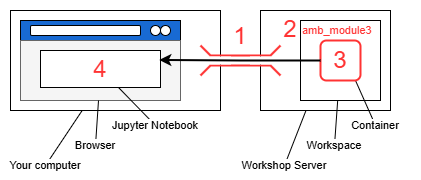
\includegraphics[keepaspectratio]{img/lab3/compute_env.png}}

\begin{enumerate}
\def\labelenumi{\arabic{enumi}.}
\tightlist
\item
  Open an additional port via SSH for the new jupyter notebook
\item
  Create a new workspace directory for this lab
\item
  Unpack and start the container
\item
  Open the jupyter notebook in your browser
\end{enumerate}

\subsubsection{SSH port forwarding}\label{ssh-port-forwarding}

We will use SSH port forwarding to open the additional port.

\paragraph{Terminal (Unix/MacOS)}\label{terminal-unixmacos}

Add \texttt{-L\ 48888:localhost:48888} to the SSH command you use to connect to the server. Something like:

\begin{Shaded}
\begin{Highlighting}[numbers=left,,]
\FunctionTok{ssh} \AttributeTok{{-}L}\NormalTok{ 48888:localhost:48888 ubuntu@\#\#.uhn{-}hpc.ca }\AttributeTok{{-}i}\NormalTok{ CBW.pem}
\end{Highlighting}
\end{Shaded}

This means port \texttt{48888} on the remote server will be forwarded to your machine at \texttt{localhost:48888}.

\paragraph{Putty (Windows)}\label{putty-windows}

Modern versions of Windows should have \texttt{ssh} available through Powershell. Putty is available as a backup.

\pandocbounded{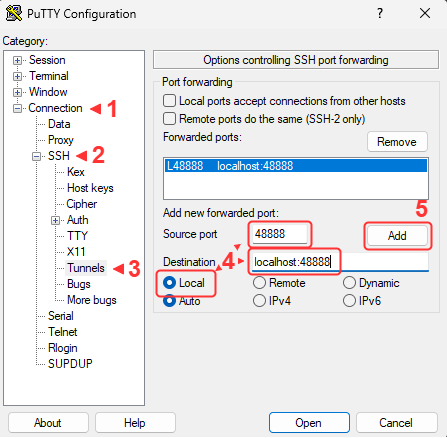
\includegraphics[keepaspectratio]{img/lab3/putty_port_forward.png}}

\subsubsection{Workspace}\label{workspace}

Let's create a new workspace for this lab.

\begin{Shaded}
\begin{Highlighting}[]
\BuiltInTok{cd}\NormalTok{ \textasciitilde{}/workspace}
\FunctionTok{mkdir}\NormalTok{ amb\_module3}
\BuiltInTok{cd}\NormalTok{ amb\_module3}
\end{Highlighting}
\end{Shaded}

Link the resource folder for easy access. This will contain all the required software and data.

\begin{Shaded}
\begin{Highlighting}[]
\FunctionTok{ln} \AttributeTok{{-}s}\NormalTok{ \textasciitilde{}/CourseData/MIC\_data/amb\_module3/ ./lib}
\end{Highlighting}
\end{Shaded}

The expected outputs for this lab can be found in \texttt{./lib/outputs}.

\begin{Shaded}
\begin{Highlighting}[]
\FunctionTok{ls}\NormalTok{ ./lib/outputs}
\end{Highlighting}
\end{Shaded}

\subsubsection{Start container}\label{start-container}

Most containers for this lab were obtained from the biocontainers project, which provides a large collection of bioinformatics software in a standard format.
For each tool, we will provide URIs for the the specific container image used and where to get future versions. At the start of each section,
you will see something like:

\begin{center}\rule{0.5\linewidth}{0.5pt}\end{center}

\url{https://quay.io/repository/biocontainers/prodigal?tab=tags}

\begin{Shaded}
\begin{Highlighting}[numbers=left,,]
\CommentTok{\# docker://quay.io/biocontainers/prodigal:2.6.3{-}{-}h7b50bb2\_10}
\NormalTok{prodigal\_sif }\OperatorTok{=}\NormalTok{ LIB}\OperatorTok{/}\StringTok{"prodigal.sif"}
\end{Highlighting}
\end{Shaded}

\begin{center}\rule{0.5\linewidth}{0.5pt}\end{center}

\begin{itemize}
\tightlist
\item
  The link (\url{https://quay.io/repository/biocontainers/prodigal?tab=tags}) will point to the container's repository for future versions.
\item
  The comment (\texttt{\#\ docker://quay.io/biocontainers/prodigal:2.6.3-\/-h7b50bb2\_10}) is the \emph{URI} for the specific version used in this lab.
\item
  The code snippet (\texttt{prodigal\_sif\ =\ LIB/"prodigal.sif"}) saves the path to the pre-downloaded container image for this lab.
\end{itemize}

After the workshop, you can use the \texttt{pull} command of \texttt{apptainer} to obtain these tools on your (linux) machine
(additional documentation: \url{https://apptainer.org/docs/user/main/cli/apptainer_pull.html}).
Here is an example for downloading the \texttt{prodigal} container image as \texttt{example.sif} from the \emph{URI} \texttt{docker://quay.io/biocontainers/prodigal:2.6.3-\/-h7b50bb2\_10}.
The image URI takes the form of \texttt{\textless{}protocol\textgreater{}://\textless{}address\textgreater{}:\textless{}tag\textgreater{}}.

\begin{Shaded}
\begin{Highlighting}[numbers=left,,]
\NormalTok{apptainer pull example.sif docker:}\OperatorTok{//}\NormalTok{quay.io}\OperatorTok{/}\NormalTok{biocontainers}\OperatorTok{/}\NormalTok{prodigal:}\FloatTok{2.6.3}\OperatorTok{{-}{-}}\NormalTok{h7b50bb2\_10}
\end{Highlighting}
\end{Shaded}

What do you think is the version of prodigal versus the prodigal container image?

Prodigal: 2.6.3. Image: 2.6.3--h7b50bb2\_10

We can now run the prodigal executable inside the container using \texttt{exec} (execute) like so.

\begin{Shaded}
\begin{Highlighting}[]
\ExtensionTok{apptainer}\NormalTok{ exec ./example.sif prodigal }\AttributeTok{{-}h}
\end{Highlighting}
\end{Shaded}

All containers for this lab were pre-downloaded in the resource folder now linked as \texttt{./lib},
including a main container with Jupyter and miscellaneous utilities (\url{https://quay.io/repository/hallamlab/cbw_amb_lab3?tab=tags}).
The main container provides an automated setup script named \texttt{unpack}. Let's run it.

\begin{Shaded}
\begin{Highlighting}[]
\ExtensionTok{apptainer}\NormalTok{ exec }\AttributeTok{{-}B}\NormalTok{ /media:/media ./lib/amb\_lab3.sif unpack}
\end{Highlighting}
\end{Shaded}

Container binds (\texttt{-B})

We need to make the container aware of the original folder linked to \texttt{./lib} so that its contents become available inside the container.
Specifically, \texttt{/media} from outside the container is bound to \texttt{/media} inside the container.

The following will dedicate the current terminal to running the juptyer notebook on port 48888.
You may want to connect another terminal to maintain terminal access.

\begin{Shaded}
\begin{Highlighting}[]
\ExtensionTok{./start\_lab}
\end{Highlighting}
\end{Shaded}

\subsubsection{Jupyter}\label{jupyter}

JupyterLab should now be accessible at \url{http://localhost:48888/lab}. Create a new python notebook and import dependencies.

\pandocbounded{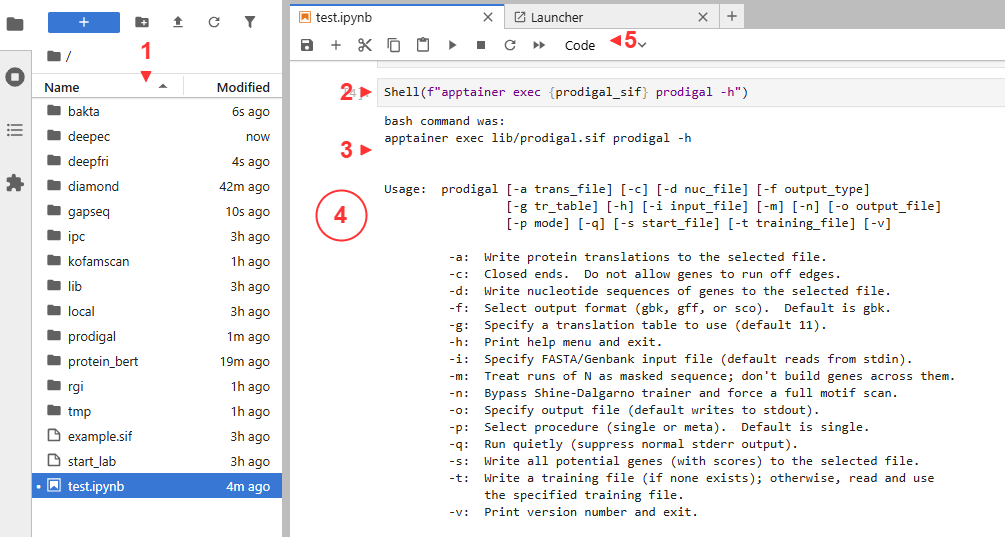
\includegraphics[keepaspectratio]{img/lab3/jupyter.png}}

\begin{enumerate}
\def\labelenumi{\arabic{enumi}.}
\tightlist
\item
  Files are on the left
\item
  Cells contain executable code
\item
  Outputs are below each cell
\item
  Clicking beside the output collapses it
\item
  Useful functions are available in the tool bar. The \texttt{+} create additional cells
\end{enumerate}

With a cell selected, you can also run it with \texttt{Shift+Enter}.

\begin{Shaded}
\begin{Highlighting}[numbers=left,,]
\ImportTok{import}\NormalTok{ pandas }\ImportTok{as}\NormalTok{ pd}
\ImportTok{from}\NormalTok{ pathlib }\ImportTok{import}\NormalTok{ Path}
\ImportTok{from}\NormalTok{ local.ipc }\ImportTok{import}\NormalTok{ Shell}

\NormalTok{LIB }\OperatorTok{=}\NormalTok{ Path(}\StringTok{"./lib"}\NormalTok{)}
\NormalTok{CPUS }\OperatorTok{=} \DecValTok{4} \CommentTok{\# your workshop instance has been alloted 4 cores}
\end{Highlighting}
\end{Shaded}

\begin{itemize}
\tightlist
\item
  \texttt{pandas} enables parsing and reading of tables
\item
  \texttt{pathlib} enables manipulation of filesystem paths
\item
  Pre-downloaded container images are in \texttt{LIB}
\item
  Pre-computed outputs for this lab are available at \texttt{LIB/"outputs"}.
\end{itemize}

Since containers can not be run inside other containers,
the provided \texttt{Shell} function grants access to the terminal outside of the main container.

\begin{Shaded}
\begin{Highlighting}[numbers=left,,]
\NormalTok{Shell(}\SpecialStringTok{f"""}
\SpecialStringTok{pwd {-}P}
\SpecialStringTok{echo }\SpecialCharTok{\{}\NormalTok{LIB}\SpecialCharTok{\}}
\SpecialStringTok{"""}\NormalTok{)}
\end{Highlighting}
\end{Shaded}

Python comments \texttt{\#\ ...}

Comments are free text not meant to be interpreted as python code and are indicated by a preceeding \texttt{\#}.
They are useful for leaving notes.

\begin{Shaded}
\begin{Highlighting}[numbers=left,,]
\CommentTok{\# \textless{}helpful information\textgreater{}}
\end{Highlighting}
\end{Shaded}

Python variables \texttt{CPUS\ =\ 4}

Useful values can be saved to variables using \texttt{=} for later use.

\begin{Shaded}
\begin{Highlighting}[numbers=left,,]
\NormalTok{x }\OperatorTok{=} \DecValTok{1} \CommentTok{\# the "value" 1 is assigned to the "variable" x}
\end{Highlighting}
\end{Shaded}

Python functions \texttt{Shell(...)}

Functions are saved procedures that can be repeatedly executed through ``calls''.
Some functions recieve additional information as ``arguments'' or ``return'' information back when called.
Called functions execute their procedure and are ``evaluated'' to their return value.
Functions without a return evaluate to the dedicated null value \texttt{None}.

\begin{Shaded}
\begin{Highlighting}[numbers=left,,]
\CommentTok{\# function definition syntax}
\KeywordTok{def}\NormalTok{ function\_name(): }\CommentTok{\# no arguments}
    \ControlFlowTok{pass} \CommentTok{\# do nothing, return nothing}

\CommentTok{\# define the function "add"}
\KeywordTok{def}\NormalTok{ add(a, b):}
    \ControlFlowTok{return}\NormalTok{ a }\OperatorTok{+}\NormalTok{ b}

\CommentTok{\# call function "add"}
\NormalTok{x }\OperatorTok{=}\NormalTok{ add(}\DecValTok{1}\NormalTok{, }\DecValTok{2}\NormalTok{) }\CommentTok{\# add evaluates to 1 + 2, then to 3, then is assigned to x}
\NormalTok{x }\CommentTok{\# x is 3}
\end{Highlighting}
\end{Shaded}

\texttt{Shell} accepts text and executes it as a bash command.

Python \texttt{import} and dot notation \texttt{local.ipc}

\begin{Shaded}
\begin{Highlighting}[numbers=left,,]
\ImportTok{from}\NormalTok{ local.ipc }\ImportTok{import}\NormalTok{ Shell }\CommentTok{\# access "ipc" from "local"}
\end{Highlighting}
\end{Shaded}

\texttt{local} is a folder containing the file \texttt{ipc.py}, which in turn defines the function \texttt{Shell}.
\texttt{local} is a python ``module'' and \texttt{ipc.py} is a python ``script''.
\texttt{import} makes python components available from other files, typically called ``libraries''.
Dot notation (the period between \texttt{local} and \texttt{ipc}) retrieves the named components of complex objects.
An alternative syntax to the above is:

\begin{Shaded}
\begin{Highlighting}[numbers=left,,]
\ImportTok{import}\NormalTok{ local.ipc.Shell }\CommentTok{\# retrieve Shell from ipc in local}
\end{Highlighting}
\end{Shaded}

imported components can be renamed using the \texttt{as} keyword:

\begin{Shaded}
\begin{Highlighting}[numbers=left,,]
\ImportTok{import}\NormalTok{ local.ipc.Shell }\ImportTok{as}\NormalTok{ Terminal }\CommentTok{\# Shell is now "Terminal"}
\end{Highlighting}
\end{Shaded}

Python strings \texttt{f"..."}

Text values in python (strings), such as the contents of a bash command, must be declared in quotes like \texttt{"text"} or \texttt{\textquotesingle{}text\textquotesingle{}}.
Triple quotes allows multi-line strings. The \texttt{f} prefix enables the evaluation of python variables in the string.
For example, \texttt{f"echo\ \{LIB\}"} evaluates to \texttt{echo\ ./lib}.
This is a convient way to simplify commands by saving repeated sections to variables.

\subsection{Overview}\label{overview-1}

This lab will guide you through finding and identifying the functional units encoded in the assembled metagenome from the previous labs
(represented by the red and orange features below), with a focus on proteins and enzymes.

\pandocbounded{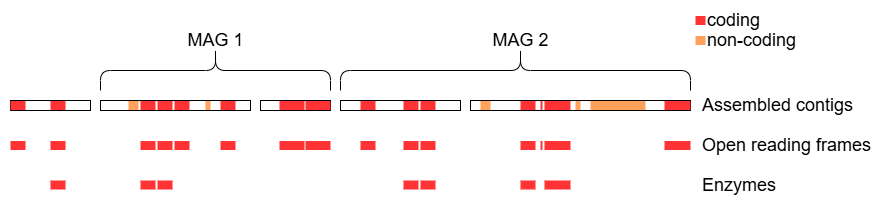
\includegraphics[keepaspectratio]{img/lab3/data_layout.png}}

We will begin by exploring techniques related to sequence similarity, which seeks to identify known genes through comparison with reference databases.

\begin{itemize}
\tightlist
\item
  \hyperref[prodigal]{Prodigal}
\item
  \hyperref[diamond]{Diamond}
\item
  \hyperref[bakta]{Bakta}
\item
  \hyperref[resistance-gene-identifier-rgi]{Resistance Gene Identifier (RGI)}
\end{itemize}

Then we will transition to machine-learning tools, which move away from the ``lookup table'' approach of sequence similarity and towards
having an internal model that ``understands'' biology.

\begin{itemize}
\tightlist
\item
  \hyperref[kofamscan]{Kofamscan}
\item
  \hyperref[deepfri]{deepFRI}
\item
  \hyperref[deepec]{deepEC}
\item
  \hyperref[proteinbert]{proteinBERT}
\end{itemize}

Finally, we will use gapseq to construct metabolic models from the given MAGs.

\begin{itemize}
\tightlist
\item
  \hyperref[gapseq]{gapseq}
\end{itemize}

\subsection{Prodigal}\label{prodigal}

The container image for prodigal:

\url{https://quay.io/repository/biocontainers/prodigal?tab=tags}

\begin{Shaded}
\begin{Highlighting}[numbers=left,,]
\CommentTok{\# docker://quay.io/biocontainers/prodigal:2.6.3{-}{-}h7b50bb2\_10}
\NormalTok{prodigal\_sif }\OperatorTok{=}\NormalTok{ LIB}\OperatorTok{/}\StringTok{"prodigal.sif"}
\end{Highlighting}
\end{Shaded}

How could you get prodigal for yourself?

\begin{enumerate}
\def\labelenumi{\arabic{enumi}.}
\tightlist
\item
  Acquire apptainer (\url{https://apptainer.org/docs/user/main/index.html})
\item
  \texttt{apptainer\ pull\ prodigal.sif\ docker://quay.io/biocontainers/prodigal:2.6.3-\/-h7b50bb2\_10}
\end{enumerate}

\begin{center}\rule{0.5\linewidth}{0.5pt}\end{center}

The goal of prodigal is to predict the protein coding features (open reading frames; ORFs) in a given nucleotide sequence.
Recall that this corresponds to the red features in the overview diagram, neglecting the orange features for now.
It does this by optimizing predictions based on a set of tuned rules (heuristics) which take into account
gene length and overlap, start and stop codons, ribosome binding sites, and GC content {[}1{]}.

\begin{enumerate}
\def\labelenumi{\arabic{enumi}.}
\tightlist
\item
  Hyatt D, Chen GL, LoCascio PF, Land ML, Larimer FW, Hauser LJ. Prodigal: prokaryotic gene recognition and translation initiation site identification. BMC Bioinformatics. 2010;11(1):119. \url{https://doi.org/10.1186/1471-2105-11-119}
\end{enumerate}

Based on this, we would expect prodigal to:

\begin{itemize}
\tightlist
\item
  accept a nucleotide sequence as input
\item
  output an itemized list of predicted open reading frames
\end{itemize}

Let's have a look at prodigal's help message to get an idea of specific inputs and outputs.

\begin{Shaded}
\begin{Highlighting}[numbers=left,,]
\NormalTok{Shell(}\SpecialStringTok{f"apptainer exec {-}B /media:/media }\SpecialCharTok{\{}\NormalTok{prodigal\_sif}\SpecialCharTok{\}}\SpecialStringTok{ prodigal {-}h"}\NormalTok{)}
\end{Highlighting}
\end{Shaded}

This looks like the input:

\begin{itemize}
\tightlist
\item
  \texttt{-i:\ \ Specify\ FASTA/Genbank\ input\ file\ (default\ reads\ from\ stdin).}
\end{itemize}

These look like they are useful for the output:

\begin{itemize}
\tightlist
\item
  \texttt{-a:\ \ Write\ protein\ translations\ to\ the\ selected\ file.}
\item
  \texttt{-d:\ \ Write\ nucleotide\ sequences\ of\ genes\ to\ the\ selected\ file.} These will be helpful next lab for aligning transcripts to genes.
\item
  \texttt{-f:\ \ Select\ output\ format\ (gbk,\ gff,\ or\ sco).\ \ Default\ is\ gbk.} We will choose \texttt{gff} since the genbank output of prodigal is not in a standard formatted.
\item
  \texttt{-o:\ \ Specify\ output\ file\ (default\ writes\ to\ stdout).}
\end{itemize}

After a bit of investigation, it also looks like we should specify that the input is a mixed population (metagenomic).

\begin{itemize}
\tightlist
\item
  \texttt{-p:\ \ Select\ procedure\ (single\ or\ meta).\ \ Default\ is\ single.}
\end{itemize}

Have a go at compiling the final command.

\begin{Shaded}
\begin{Highlighting}[numbers=left,,]
\NormalTok{out\_dir }\OperatorTok{=} \StringTok{"./prodigal"}
\NormalTok{Shell(}\SpecialStringTok{f"""}
\SpecialStringTok{mkdir {-}p }\SpecialCharTok{\{}\NormalTok{out\_dir}\SpecialCharTok{\}}\SpecialStringTok{/}
\SpecialStringTok{apptainer exec {-}B /media:/media }\SpecialCharTok{\{}\NormalTok{prodigal\_sif}\SpecialCharTok{\}}\SpecialStringTok{ }\CharTok{\textbackslash{}}
\SpecialStringTok{    prodigal }\CharTok{\textbackslash{}}
\SpecialStringTok{        {-}i }\SpecialCharTok{\{}\NormalTok{LIB}\SpecialCharTok{\}}\SpecialStringTok{/inputs/assembly.fa }\CharTok{\textbackslash{}}
\SpecialStringTok{        ...}
\SpecialStringTok{"""}\NormalTok{)}
\end{Highlighting}
\end{Shaded}

The purpose of \texttt{\textbackslash{}}

Starting from \texttt{apptainer\ exec}, the command must be written in a single line.
The backslash \texttt{\textbackslash{}} is used to ignore the newline character and continue the command on the next line.
This let's us write break up a long command into multiple lines for readability.
---

Why wouldn't we want to use the MAGs as input?

Not all contigs of the metagenomic assembly are in MAGs.

\begin{center}\rule{0.5\linewidth}{0.5pt}\end{center}

Suggested answer

\begin{Shaded}
\begin{Highlighting}[numbers=left,,]
\NormalTok{out\_dir }\OperatorTok{=}\NormalTok{ Path(}\StringTok{"./prodigal"}\NormalTok{)}
\NormalTok{prodigal\_aa }\OperatorTok{=}\NormalTok{ out\_dir}\OperatorTok{/}\StringTok{"orfs.faa"}
\NormalTok{prodigal\_gff }\OperatorTok{=}\NormalTok{ out\_dir}\OperatorTok{/}\StringTok{"orfs.gff"}
\NormalTok{Shell(}\SpecialStringTok{f"""}\CharTok{\textbackslash{}}
\SpecialStringTok{mkdir {-}p }\SpecialCharTok{\{}\NormalTok{out\_dir}\SpecialCharTok{\}}\SpecialStringTok{/}
\SpecialStringTok{apptainer exec {-}B /media:/media }\SpecialCharTok{\{}\NormalTok{prodigal\_sif}\SpecialCharTok{\}}\SpecialStringTok{ }\CharTok{\textbackslash{}}
\SpecialStringTok{    prodigal }\CharTok{\textbackslash{}}
\SpecialStringTok{        {-}p meta }\CharTok{\textbackslash{}}
\SpecialStringTok{        {-}i }\SpecialCharTok{\{}\NormalTok{LIB}\SpecialCharTok{\}}\SpecialStringTok{/inputs/assembly.fa }\CharTok{\textbackslash{}}
\SpecialStringTok{        {-}a }\SpecialCharTok{\{}\NormalTok{prodigal\_aa}\SpecialCharTok{\}}\SpecialStringTok{ }\CharTok{\textbackslash{}}
\SpecialStringTok{        {-}d }\SpecialCharTok{\{}\NormalTok{prodigal\_aa}\SpecialCharTok{.}\NormalTok{with\_suffix(}\StringTok{\textquotesingle{}.fna\textquotesingle{}}\NormalTok{)}\SpecialCharTok{\}}\SpecialStringTok{ }\CharTok{\textbackslash{}}
\SpecialStringTok{        {-}f gff }\CharTok{\textbackslash{}}
\SpecialStringTok{        {-}o }\SpecialCharTok{\{}\NormalTok{prodigal\_gff}\SpecialCharTok{\}}\SpecialStringTok{ }\CharTok{\textbackslash{}}
\SpecialStringTok{"""}\NormalTok{)}
\end{Highlighting}
\end{Shaded}

\begin{center}\rule{0.5\linewidth}{0.5pt}\end{center}

Let's take a peek at the gene feature format (\texttt{gff}) file.

\begin{Shaded}
\begin{Highlighting}[numbers=left,,]
\NormalTok{gff }\OperatorTok{=}\NormalTok{ pd.read\_csv(out\_dir}\OperatorTok{/}\StringTok{"orfs.gff"}\NormalTok{, sep}\OperatorTok{=}\StringTok{"}\CharTok{\textbackslash{}t}\StringTok{"}\NormalTok{, header}\OperatorTok{=}\VariableTok{None}\NormalTok{, comment}\OperatorTok{=}\StringTok{"\#"}\NormalTok{)}
\BuiltInTok{print}\NormalTok{(gff.shape)}
\NormalTok{gff.head(}\DecValTok{2}\NormalTok{)}
\end{Highlighting}
\end{Shaded}

From left to right, the columns are:

\begin{enumerate}
\def\labelenumi{\arabic{enumi}.}
\setcounter{enumi}{-1}
\tightlist
\item
  contig id
\item
  name of the program that generated this feature
\item
  feature type, where \texttt{CDS} stands for coding sequence
\item
  start position (first nucleotide is 1)
\item
  end position
\item
  raw prodigal score
\item
  strand, where \texttt{+} is forward and \texttt{-} is reverse
\item
  codon frame, being one of 0, 1 or 2
\item
  a semicolon-separated list of tag-value pairs, providing additional information about each feature
\end{enumerate}

Selecting entries in python dataframes and matrices

Entries (rows, columns, or cells) in pandas dataframes and numpy matricies can be selected in multiple ways.

Example matrix:

\begin{Shaded}
\begin{Highlighting}[numbers=left,,]
\NormalTok{mat }\OperatorTok{=}\NormalTok{ np.array([}\DecValTok{1}\NormalTok{, }\DecValTok{2}\NormalTok{, }\DecValTok{3}\NormalTok{, }\DecValTok{4}\NormalTok{, }\DecValTok{5}\NormalTok{])}
\end{Highlighting}
\end{Shaded}

Select by single index, where negative indexes count from the end:

\begin{Shaded}
\begin{Highlighting}[numbers=left,,]
\NormalTok{mat[}\DecValTok{0}\NormalTok{]      }\CommentTok{\# 1}
\NormalTok{mat[}\OperatorTok{{-}}\DecValTok{1}\NormalTok{]     }\CommentTok{\# 5}
\end{Highlighting}
\end{Shaded}

a slice in the form of \texttt{start:end}, where \texttt{start} is inclusive and \texttt{end} is exclusive:

\begin{Shaded}
\begin{Highlighting}[numbers=left,,]
\NormalTok{mat[}\DecValTok{1}\NormalTok{:}\DecValTok{4}\NormalTok{]    }\CommentTok{\# [2, 3, 4]}
\NormalTok{mat[:}\DecValTok{2}\NormalTok{]     }\CommentTok{\# [1, 2]}
\NormalTok{mat[}\DecValTok{2}\NormalTok{:]     }\CommentTok{\# [3, 4, 5]}
\NormalTok{mat[}\OperatorTok{{-}}\DecValTok{1}\NormalTok{:]    }\CommentTok{\# [5]}
\end{Highlighting}
\end{Shaded}

a list of indexes:

\begin{Shaded}
\begin{Highlighting}[numbers=left,,]
\NormalTok{mat[[}\DecValTok{0}\NormalTok{, }\DecValTok{2}\NormalTok{, }\DecValTok{4}\NormalTok{]] }\CommentTok{\# [1, 3, 5]}
\end{Highlighting}
\end{Shaded}

a boolean mask:

\begin{Shaded}
\begin{Highlighting}[numbers=left,,]
\NormalTok{mat[[}\VariableTok{False}\NormalTok{, }\VariableTok{False}\NormalTok{, }\VariableTok{False}\NormalTok{, }\VariableTok{True}\NormalTok{, }\VariableTok{True}\NormalTok{]] }\CommentTok{\# [4, 5]}
\end{Highlighting}
\end{Shaded}

\begin{center}\rule{0.5\linewidth}{0.5pt}\end{center}

Let's investigate how many ORFs were not in MAGs. To do this, we will first create a blacklist for mag contig IDs.

\begin{Shaded}
\begin{Highlighting}[numbers=left,,]
\ImportTok{from}\NormalTok{ Bio }\ImportTok{import}\NormalTok{ SeqIO }\CommentTok{\# SeqIO from Biopython enables us to read fasta files, among other formats}
\CommentTok{\# https://biopython.org/wiki/SeqIO\#:\textasciitilde{}:text=Peter{-},File\%20Formats,{-}The\%20authorative\%20list}

\NormalTok{mag\_ids }\OperatorTok{=} \BuiltInTok{set}\NormalTok{()}
\CommentTok{\# loop through the paths to each of the MAG files}
\ControlFlowTok{for}\NormalTok{ mag\_file }\KeywordTok{in}\NormalTok{ [}
\NormalTok{    LIB}\OperatorTok{/}\StringTok{"inputs/HMP2\_MAG\_00001{-}contigs.fa"}\NormalTok{,}
\NormalTok{    LIB}\OperatorTok{/}\StringTok{"inputs/HMP2\_MAG\_00002{-}contigs.fa"}\NormalTok{,}
\NormalTok{]:}
    \CommentTok{\# we can use SeqIO to iterate through each sequence in a fasta file}
    \ControlFlowTok{for}\NormalTok{ contig }\KeywordTok{in}\NormalTok{ SeqIO.parse(mag\_file, }\StringTok{"fasta"}\NormalTok{):}
\NormalTok{        mag\_ids.add(contig.}\BuiltInTok{id}\NormalTok{) }\CommentTok{\# add the contig id of each contig to mag\_ids}
\BuiltInTok{len}\NormalTok{(mag\_ids)}
\end{Highlighting}
\end{Shaded}

Python \texttt{for} loops

Loops enable repeated execution of a block of code for each element in a collection.

\begin{Shaded}
\begin{Highlighting}[numbers=left,,]
\NormalTok{collection }\OperatorTok{=}\NormalTok{ [}\DecValTok{1}\NormalTok{, }\DecValTok{2}\NormalTok{, }\DecValTok{3}\NormalTok{] }\CommentTok{\# a "list" collection}
\ControlFlowTok{for}\NormalTok{ element }\KeywordTok{in}\NormalTok{ collection:}
    \BuiltInTok{print}\NormalTok{(element) }\CommentTok{\# do something with each element}

\CommentTok{\# result:}
\CommentTok{\# 1}
\CommentTok{\# 2}
\CommentTok{\# 3}
\end{Highlighting}
\end{Shaded}

Then filter the gff based on the MAG blacklist.

\begin{Shaded}
\begin{Highlighting}[numbers=left,,]
\NormalTok{\_filter }\OperatorTok{=} \OperatorTok{\textasciitilde{}}\NormalTok{gff[}\DecValTok{0}\NormalTok{].isin(mag\_ids) }\CommentTok{\# column 0 is the contig id}
\NormalTok{non\_mag\_orfs }\OperatorTok{=}\NormalTok{ gff[\_filter]}
\NormalTok{non\_mag\_orfs.shape}
\end{Highlighting}
\end{Shaded}

How many contigs were in MAGs?

803

How many ORFs were not from MAGs?

1060 of 7176, or about 15\%

\subsection{Sequence similarity}\label{sequence-similarity}

In this section, we will use tools to find proteins with known sequences similar to that of the predicted ORFs.
By assuming similar sequences equate to similar functions, we can assign functions through reference databases of known proteins.
While not perfect {[}1, 2{]}, this is a common first-pass approach to assign functions to genes in metagenomic assemblies.

\begin{enumerate}
\def\labelenumi{\arabic{enumi}.}
\tightlist
\item
  Omelchenko MV, Galperin MY, Wolf YI, Koonin EV. Non-homologous isofunctional enzymes: A systematic analysis of alternative solutions in enzyme evolution. Biol Direct. 2010;5(1):31. \url{https://doi.org/10.1186/1745-6150-5-31}
\item
  Seffernick JL, de Souza ML, Sadowsky MJ, Wackett LP. Melamine deaminase and atrazine chlorohydrolase: 98 percent identical but functionally different. J Bacteriol. 2001;183(8):2405--10. \url{https://doi.org/10.1128/JB.183.8.2405-2410.2001}
\end{enumerate}

\subsubsection{Diamond}\label{diamond}

\url{https://quay.io/repository/biocontainers/diamond?tab=tags}

\begin{Shaded}
\begin{Highlighting}[numbers=left,,]
\CommentTok{\# docker://quay.io/biocontainers/diamond:2.1.11{-}{-}h5ca1c30\_2}
\NormalTok{diamond\_sif }\OperatorTok{=}\NormalTok{ LIB}\OperatorTok{/}\StringTok{"diamond.sif"}
\end{Highlighting}
\end{Shaded}

Diamond is highly optimized for finding similar protein sequences between a list of queries and a list of subjects {[}1{]}.
It has a similar command line interface (CLI) to the classic BLAST, requiring that we first build a database from the list of subjects,
before searching against it with a list of queries.

\begin{enumerate}
\def\labelenumi{\arabic{enumi}.}
\tightlist
\item
  Buchfink B, Xie C, Huson DH. Fast and sensitive protein alignment using DIAMOND. Nat Methods. 2015;12(1):59--60. \url{https://doi.org/10.1038/nmeth.3176}
\end{enumerate}

We expect to run diamond in two steps:

\begin{enumerate}
\def\labelenumi{\arabic{enumi}.}
\tightlist
\item
  Build a reference database

  \begin{itemize}
  \tightlist
  \item
    inputs: a list of protein sequences
  \item
    outputs: a database file
  \end{itemize}
\item
  Search the database

  \begin{itemize}
  \tightlist
  \item
    inputs: a list of protein sequences, the compiled database
  \item
    outputs: a list of hits
  \end{itemize}
\end{enumerate}

\begin{Shaded}
\begin{Highlighting}[numbers=left,,]
\NormalTok{Shell(}\SpecialStringTok{f"apptainer exec {-}B /media:/media }\SpecialCharTok{\{}\NormalTok{diamond\_sif}\SpecialCharTok{\}}\SpecialStringTok{ diamond {-}{-}help"}\NormalTok{)}
\end{Highlighting}
\end{Shaded}

We will build a database for transporters using the transporter classification database (TCDB) {[}1{]}.
TCDB has been predownloaded from these URLs.

\begin{itemize}
\tightlist
\item
  protein sequences: \url{https://www.tcdb.org/public/tcdb}
\item
  sequences are grouped into families: \url{https://www.tcdb.org/cgi-bin/projectv/public/families.py}
\item
  transporter substrates: \url{https://www.tcdb.org/cgi-bin/substrates/getSubstrates.py}
\end{itemize}

\begin{enumerate}
\def\labelenumi{\arabic{enumi}.}
\tightlist
\item
  Saier MH Jr, Tran CV, Barabote RD. TCDB: the Transporter Classification Database for membrane transport protein analyses and information. Nucleic Acids Res. 2006;34(suppl\_1):D181--6. \url{https://doi.org/10.1093/nar/gkj001}
\end{enumerate}

\begin{Shaded}
\begin{Highlighting}[numbers=left,,]
\NormalTok{Shell(}\SpecialStringTok{f"apptainer exec {-}B /media:/media }\SpecialCharTok{\{}\NormalTok{diamond\_sif}\SpecialCharTok{\}}\SpecialStringTok{ diamond makedb"}\NormalTok{)}
\end{Highlighting}
\end{Shaded}

The important arguments appear to be:

\begin{itemize}
\tightlist
\item
  \texttt{-\/-db\ \ \ \ \ \ \ \ \ \ \ \ \ \ \ \ \ \ \ \ \ database\ file}
\item
  \texttt{-\/-in\ \ \ \ \ \ \ \ \ \ \ \ \ \ \ \ \ \ \ \ \ input\ reference\ file\ in\ FASTA\ format/input\ DAA\ files\ for\ merge-daa}
\end{itemize}

Have a go at compiling the command to build the diamond database.
Running a your command is a good way to check for correctness and resulting error messages can be informative.

\begin{Shaded}
\begin{Highlighting}[numbers=left,,]
\NormalTok{tcdb\_fasta }\OperatorTok{=}\NormalTok{ LIB}\OperatorTok{/}\StringTok{"transporter\_classification\_db/tcdb.faa"}
\NormalTok{tcdb\_db }\OperatorTok{=}\NormalTok{ Path(}\StringTok{"./diamond/tcdb.dmnd"}\NormalTok{)}
\NormalTok{Shell(}\SpecialStringTok{f"""}
\SpecialStringTok{apptainer exec {-}B /media:/media }\SpecialCharTok{\{}\NormalTok{diamond\_sif}\SpecialCharTok{\}}\SpecialStringTok{ diamond makedb }\CharTok{\textbackslash{}}
\SpecialStringTok{    ...}
\SpecialStringTok{"""}\NormalTok{)}
\end{Highlighting}
\end{Shaded}

Possible solution

\begin{Shaded}
\begin{Highlighting}[numbers=left,,]
\NormalTok{tcdb\_fasta }\OperatorTok{=}\NormalTok{ LIB}\OperatorTok{/}\StringTok{"transporter\_classification\_db/tcdb.faa"}
\NormalTok{tcdb\_db }\OperatorTok{=}\NormalTok{ Path(}\StringTok{"./diamond/tcdb.dmnd"}\NormalTok{)}
\NormalTok{Shell(}\SpecialStringTok{f"""}
\SpecialStringTok{mkdir {-}p }\SpecialCharTok{\{}\NormalTok{tcdb\_db}\SpecialCharTok{.}\NormalTok{parent}\SpecialCharTok{\}}\SpecialStringTok{ \# parent folder of given path}
\SpecialStringTok{apptainer exec {-}B /media:/media }\SpecialCharTok{\{}\NormalTok{diamond\_sif}\SpecialCharTok{\}}\SpecialStringTok{ diamond makedb }\CharTok{\textbackslash{}}
\SpecialStringTok{    {-}{-}threads }\SpecialCharTok{\{}\NormalTok{CPUS}\SpecialCharTok{\}}\SpecialStringTok{ }\CharTok{\textbackslash{}}
\SpecialStringTok{    {-}{-}in }\SpecialCharTok{\{}\NormalTok{tcdb\_fasta}\SpecialCharTok{\}}\SpecialStringTok{ }\CharTok{\textbackslash{}}
\SpecialStringTok{    {-}{-}db }\SpecialCharTok{\{}\NormalTok{tcdb\_db}\SpecialCharTok{\}}
\SpecialStringTok{"""}\NormalTok{)}
\end{Highlighting}
\end{Shaded}

Now we can search our predicted ORFs for transporters catalogued in TCDB.

\begin{Shaded}
\begin{Highlighting}[numbers=left,,]
\NormalTok{Shell(}\SpecialStringTok{f"apptainer exec {-}B /media:/media }\SpecialCharTok{\{}\NormalTok{diamond\_sif}\SpecialCharTok{\}}\SpecialStringTok{ diamond blastp"}\NormalTok{)}
\end{Highlighting}
\end{Shaded}

That produced a lot of output, but these are the essential arguments:

\begin{itemize}
\tightlist
\item
  \texttt{-\/-query\ \ \ \ \ \ \ \ \ \ \ \ \ \ \ \ \ \ input\ query\ file}
\item
  \texttt{-\/-db\ \ \ \ \ \ \ \ \ \ \ \ \ \ \ \ \ \ \ \ \ database\ file}
\item
  \texttt{-\/-out\ \ \ \ \ \ \ \ \ \ \ \ \ \ \ \ \ \ \ \ output\ file}
\end{itemize}

These may be frequently useful:

\begin{itemize}
\tightlist
\item
  \texttt{-\/-fast\ \ \ \ \ \ \ \ \ \ \ \ \ \ \ \ \ \ \ enable\ fast\ mode}
\item
  \texttt{-\/-sensitive\ \ \ \ \ \ \ \ \ \ \ \ \ \ enable\ sensitive\ mode}
\item
  \texttt{-\/-ultra-sensitive\ \ \ \ \ \ \ \ enable\ ultra\ sensitive\ mode}
\item
  \texttt{-\/-threads\ \ \ \ \ \ \ \ \ \ \ \ \ \ \ \ number\ of\ CPU\ threads}
\item
  \texttt{-\/-outfmt\ \ \ \ \ \ \ \ \ \ \ \ \ \ \ \ \ output\ format}
\item
  \texttt{-\/-evalue\ \ \ \ \ \ \ \ \ \ \ \ \ \ \ \ \ maximum\ e-value\ to\ report\ alignments\ (default=0.001)}
\end{itemize}

I find that this works well for general cases.

\begin{Shaded}
\begin{Highlighting}[numbers=left,,]
\NormalTok{columns }\OperatorTok{=} \StringTok{"qseqid sseqid score pident evalue"}
\NormalTok{diamond\_out }\OperatorTok{=}\NormalTok{ Path(}\StringTok{"./diamond/orfs.tsv"}\NormalTok{)}
\NormalTok{Shell(}\SpecialStringTok{f"""}
\SpecialStringTok{apptainer exec {-}B /media:/media }\SpecialCharTok{\{}\NormalTok{diamond\_sif}\SpecialCharTok{\}}\SpecialStringTok{ }\CharTok{\textbackslash{}}
\SpecialStringTok{    diamond blastp }\CharTok{\textbackslash{}}
\SpecialStringTok{        {-}{-}query ./prodigal/orfs.faa }\CharTok{\textbackslash{}}
\SpecialStringTok{        {-}{-}db }\SpecialCharTok{\{}\NormalTok{tcdb\_db}\SpecialCharTok{\}}\SpecialStringTok{ }\CharTok{\textbackslash{}}
\SpecialStringTok{        {-}{-}out }\SpecialCharTok{\{}\NormalTok{diamond\_out}\SpecialCharTok{\}}\SpecialStringTok{ }\CharTok{\textbackslash{}}
\SpecialStringTok{        {-}{-}outfmt 6 }\SpecialCharTok{\{}\NormalTok{columns}\SpecialCharTok{\}}\SpecialStringTok{ }\CharTok{\textbackslash{}}
\SpecialStringTok{        {-}{-}threads }\SpecialCharTok{\{}\NormalTok{CPUS}\SpecialCharTok{\}}
\SpecialStringTok{"""}\NormalTok{)}
\end{Highlighting}
\end{Shaded}

In addition to e-evalue, we can calculate a blast score ratio (BSR) to assign confidence to the hits.
BSR for a hit is defined as the ratio of its score to the score of the query aligned to itself (the best possible score).
A BSR of less than 0.4 was found to be a good threshold {[}1{]}.

\begin{enumerate}
\def\labelenumi{\arabic{enumi}.}
\tightlist
\item
  Rost B. Twilight zone of protein sequence alignments. Protein Eng. 1999;12(2):85--94. \url{https://doi.org/10.1093/protein/12.2.85}
\end{enumerate}

Perform a self blast. We can skip making a database since the number of sequences is small.

\begin{Shaded}
\begin{Highlighting}[numbers=left,,]
\NormalTok{diamond\_self }\OperatorTok{=}\NormalTok{ Path(}\StringTok{"./diamond/self.raw"}\NormalTok{)}
\NormalTok{Shell(}\SpecialStringTok{f"""}
\SpecialStringTok{apptainer exec {-}B /media:/media }\SpecialCharTok{\{}\NormalTok{diamond\_sif}\SpecialCharTok{\}}\SpecialStringTok{ }\CharTok{\textbackslash{}}
\SpecialStringTok{    diamond blastp }\CharTok{\textbackslash{}}
\SpecialStringTok{        {-}{-}query }\SpecialCharTok{\{}\NormalTok{prodigal\_aa}\SpecialCharTok{\}}\SpecialStringTok{ }\CharTok{\textbackslash{}}
\SpecialStringTok{        {-}{-}db }\SpecialCharTok{\{}\NormalTok{prodigal\_aa}\SpecialCharTok{\}}\SpecialStringTok{ }\CharTok{\textbackslash{}}
\SpecialStringTok{        {-}{-}out }\SpecialCharTok{\{}\NormalTok{diamond\_self}\SpecialCharTok{\}}\SpecialStringTok{ }\CharTok{\textbackslash{}}
\SpecialStringTok{        {-}{-}outfmt 6 }\SpecialCharTok{\{}\NormalTok{columns}\SpecialCharTok{\}}\SpecialStringTok{ }\CharTok{\textbackslash{}}
\SpecialStringTok{        {-}{-}max{-}target{-}seqs 1 }\CharTok{\textbackslash{}}
\SpecialStringTok{        {-}{-}faster }\CharTok{\textbackslash{}}
\SpecialStringTok{        {-}{-}threads }\SpecialCharTok{\{}\NormalTok{CPUS}\SpecialCharTok{\}}
\SpecialStringTok{"""}\NormalTok{)}
\end{Highlighting}
\end{Shaded}

``string''.split() and ``string''.join()

Strings can be split into lists using the \texttt{split} method.

\begin{Shaded}
\begin{Highlighting}[numbers=left,,]
\CommentTok{"a b c"}\NormalTok{.split(}\StringTok{" "}\NormalTok{) }\CommentTok{\# ["a", "b", "c"]}
\CommentTok{"a|b|c"}\NormalTok{.split(}\StringTok{"|"}\NormalTok{) }\CommentTok{\# ["a", "b", "c"]}
\CommentTok{"c\_001\_3"}\NormalTok{.split(}\StringTok{"\_"}\NormalTok{) }\CommentTok{\# ["c", "001", "3"]}
\end{Highlighting}
\end{Shaded}

Lists can be joined into strings using the \texttt{join} method.

\begin{Shaded}
\begin{Highlighting}[numbers=left,,]
\CommentTok{" "}\NormalTok{.join([}\StringTok{"a"}\NormalTok{, }\StringTok{"b"}\NormalTok{, }\StringTok{"c"}\NormalTok{]) }\CommentTok{\# "a b c"}
\CommentTok{"\_"}\NormalTok{.join([}\StringTok{"c"}\NormalTok{, }\StringTok{"001"}\NormalTok{]) }\CommentTok{\# "c\_001"}
\end{Highlighting}
\end{Shaded}

\begin{center}\rule{0.5\linewidth}{0.5pt}\end{center}

We now remove hits with a BSR \textless{} 0.4. First, load in the self blast results.

\begin{Shaded}
\begin{Highlighting}[numbers=left,,]
\CommentTok{\# get self scores}
\NormalTok{df\_self }\OperatorTok{=}\NormalTok{ pd.read\_csv(diamond\_self, sep}\OperatorTok{=}\StringTok{"}\CharTok{\textbackslash{}t}\StringTok{"}\NormalTok{, header}\OperatorTok{=}\VariableTok{None}\NormalTok{, names}\OperatorTok{=}\NormalTok{columns.split(}\StringTok{" "}\NormalTok{))}
\NormalTok{df\_self }\OperatorTok{=}\NormalTok{ df\_self[df\_self[}\StringTok{"qseqid"}\NormalTok{] }\OperatorTok{==}\NormalTok{ df\_self[}\StringTok{"sseqid"}\NormalTok{]] }\CommentTok{\# use boolean mask to select self hits}
\BuiltInTok{print}\NormalTok{(df\_self.shape)}
\NormalTok{df\_self.head(}\DecValTok{2}\NormalTok{)}
\end{Highlighting}
\end{Shaded}

As the code gets more complex, it may be helpful to examine individual components to increase understanding.
For example, have a look at:

\begin{Shaded}
\begin{Highlighting}[numbers=left,,]
\NormalTok{columns.split(}\StringTok{" "}\NormalTok{)}
\CommentTok{\# and}
\NormalTok{df\_self[}\StringTok{"qseqid"}\NormalTok{] }\OperatorTok{==}\NormalTok{ df\_self[}\StringTok{"sseqid"}\NormalTok{]}
\CommentTok{\# or even}
\NormalTok{df\_self[}\StringTok{"qseqid"}\NormalTok{]}
\end{Highlighting}
\end{Shaded}

Calculate BSR

\begin{Shaded}
\begin{Highlighting}[numbers=left,,]
\NormalTok{df\_raw }\OperatorTok{=}\NormalTok{ pd.read\_csv(diamond\_out, sep}\OperatorTok{=}\StringTok{"}\CharTok{\textbackslash{}t}\StringTok{"}\NormalTok{, header}\OperatorTok{=}\VariableTok{None}\NormalTok{, names}\OperatorTok{=}\NormalTok{columns.split(}\StringTok{" "}\NormalTok{))}
\CommentTok{\# merge in self scores by matching the qseqid}
\CommentTok{\# "left" refers to a "left join" where}
\CommentTok{\# each row in the left dataframe (df\_raw) is found a match in the right (df\_self)}
\CommentTok{\# duplicate columns from the right df are suffixed with "\_self", such as "score\_self"}
\NormalTok{df\_hits }\OperatorTok{=}\NormalTok{ df\_raw.merge(df\_self, on}\OperatorTok{=}\StringTok{"qseqid"}\NormalTok{, suffixes}\OperatorTok{=}\NormalTok{(}\StringTok{""}\NormalTok{, }\StringTok{"\_self"}\NormalTok{), how}\OperatorTok{=}\StringTok{"left"}\NormalTok{)}
\CommentTok{\# calculate bsr and place in new column}
\NormalTok{df\_hits[}\StringTok{"bsr"}\NormalTok{] }\OperatorTok{=}\NormalTok{ df\_hits[}\StringTok{"score"}\NormalTok{] }\OperatorTok{/}\NormalTok{ df\_hits[}\StringTok{"score\_self"}\NormalTok{] }\CommentTok{\# divide each value in score by the corresponding value in score\_self}
\NormalTok{df\_hits.head(}\DecValTok{2}\NormalTok{)}
\end{Highlighting}
\end{Shaded}

Filter out hits with BSR \textless{} 0.4

\begin{Shaded}
\begin{Highlighting}[numbers=left,,]
\NormalTok{df\_hits }\OperatorTok{=}\NormalTok{ df\_hits[df\_hits[}\StringTok{"bsr"}\NormalTok{] }\OperatorTok{\textgreater{}=} \FloatTok{0.4}\NormalTok{] }\CommentTok{\# filter out rows with bsr \textless{} 0.4}
\NormalTok{df\_hits }\OperatorTok{=}\NormalTok{ df\_hits[columns.split(}\StringTok{" "}\NormalTok{) }\OperatorTok{+}\NormalTok{ [}\StringTok{"bsr"}\NormalTok{]] }\CommentTok{\# keep only the columns we want}
\NormalTok{df\_hits.head(}\DecValTok{2}\NormalTok{)}
\end{Highlighting}
\end{Shaded}

Take the best hit

\begin{Shaded}
\begin{Highlighting}[numbers=left,,]
\CommentTok{\# sort by bsr and group by qseqid, keeping the first row of each group}
\CommentTok{\# this will keep the best hit for each query sequence}
\CommentTok{\# groupby("qseqid") will set the index to qseqid, so we reset the index}
\NormalTok{df\_hits }\OperatorTok{=}\NormalTok{ df\_hits.sort\_values(}\StringTok{"bsr"}\NormalTok{, ascending}\OperatorTok{=}\VariableTok{False}\NormalTok{).groupby(}\StringTok{"qseqid"}\NormalTok{).first().reset\_index()}
\NormalTok{df\_hits }\OperatorTok{=}\NormalTok{ df\_hits.sort\_values(}\StringTok{"qseqid"}\NormalTok{) }\CommentTok{\# re{-}sort by qseqid}
\BuiltInTok{print}\NormalTok{(df\_hits.shape)}
\NormalTok{df\_hits.head(}\DecValTok{2}\NormalTok{)}
\end{Highlighting}
\end{Shaded}

Let's plot the results using a simple diverging bar chart for each MAG. First, let's create whitelists for the contigs in each MAG.

\begin{Shaded}
\begin{Highlighting}[numbers=left,,]
\NormalTok{MAG1 }\OperatorTok{=} \BuiltInTok{set}\NormalTok{()}
\ControlFlowTok{for}\NormalTok{ e }\KeywordTok{in}\NormalTok{ SeqIO.parse(LIB}\OperatorTok{/}\StringTok{"inputs/HMP2\_MAG\_00001{-}contigs.fa"}\NormalTok{, }\StringTok{"fasta"}\NormalTok{):}
\NormalTok{    MAG1.add(e.}\BuiltInTok{id}\NormalTok{)}
\NormalTok{MAG2 }\OperatorTok{=} \BuiltInTok{set}\NormalTok{()}
\ControlFlowTok{for}\NormalTok{ e }\KeywordTok{in}\NormalTok{ SeqIO.parse(LIB}\OperatorTok{/}\StringTok{"inputs/HMP2\_MAG\_00002{-}contigs.fa"}\NormalTok{, }\StringTok{"fasta"}\NormalTok{):}
\NormalTok{    MAG2.add(e.}\BuiltInTok{id}\NormalTok{)}
\BuiltInTok{len}\NormalTok{(MAG1), }\BuiltInTok{len}\NormalTok{(MAG2)}
\end{Highlighting}
\end{Shaded}

Python \texttt{set}

Sets enable easy checking of membership using \texttt{in}. For example:

\begin{Shaded}
\begin{Highlighting}[numbers=left,,]
\NormalTok{empty\_set }\OperatorTok{=} \BuiltInTok{set}\NormalTok{()}
\NormalTok{X }\OperatorTok{=}\NormalTok{ \{}\DecValTok{1}\NormalTok{, }\DecValTok{2}\NormalTok{, }\DecValTok{3}\NormalTok{\}}
\DecValTok{1} \KeywordTok{in}\NormalTok{ X }\CommentTok{\# True}
\DecValTok{0} \KeywordTok{in}\NormalTok{ X }\CommentTok{\# False}
\end{Highlighting}
\end{Shaded}

\begin{center}\rule{0.5\linewidth}{0.5pt}\end{center}

We can use the whitelists with additional parsing to get the family and MAG for each hit.

\begin{Shaded}
\begin{Highlighting}[numbers=left,,]
\NormalTok{\_fams }\OperatorTok{=}\NormalTok{ []}
\NormalTok{\_mags }\OperatorTok{=}\NormalTok{ []}
\NormalTok{df\_fam }\OperatorTok{=}\NormalTok{ pd.DataFrame(df\_hits)}
\ControlFlowTok{for}\NormalTok{ \_, row }\KeywordTok{in}\NormalTok{ df\_fam.iterrows():}
\NormalTok{    orf }\OperatorTok{=}\NormalTok{ row[}\StringTok{"qseqid"}\NormalTok{]}
\NormalTok{    parts }\OperatorTok{=}\NormalTok{ orf.split(}\StringTok{"\_"}\NormalTok{)}
\NormalTok{    contig }\OperatorTok{=} \StringTok{"\_"}\NormalTok{.join(parts[:}\OperatorTok{{-}}\DecValTok{1}\NormalTok{])}
    \ControlFlowTok{if}\NormalTok{ contig }\KeywordTok{in}\NormalTok{ MAG1:}
\NormalTok{        mag }\OperatorTok{=} \DecValTok{1}
    \ControlFlowTok{elif}\NormalTok{ contig }\KeywordTok{in}\NormalTok{ MAG2:}
\NormalTok{        mag }\OperatorTok{=} \DecValTok{2}
    \ControlFlowTok{else}\NormalTok{:}
\NormalTok{        mag }\OperatorTok{=} \DecValTok{0} \CommentTok{\# not in either MAG}
\NormalTok{    \_mags.append(mag)}

\NormalTok{    description }\OperatorTok{=}\NormalTok{ row[}\StringTok{"sseqid"}\NormalTok{]}
\NormalTok{    tcdb\_id }\OperatorTok{=}\NormalTok{ description.split(}\StringTok{"|"}\NormalTok{)[}\OperatorTok{{-}}\DecValTok{1}\NormalTok{]}
\NormalTok{    parts }\OperatorTok{=}\NormalTok{ tcdb\_id.split(}\StringTok{"."}\NormalTok{)}
\NormalTok{    family }\OperatorTok{=} \StringTok{"."}\NormalTok{.join(parts[:}\DecValTok{3}\NormalTok{])}
\NormalTok{    \_fams.append(family)}

\NormalTok{df\_fam[}\StringTok{"family"}\NormalTok{] }\OperatorTok{=}\NormalTok{ \_fams}
\NormalTok{df\_fam[}\StringTok{"mag"}\NormalTok{] }\OperatorTok{=}\NormalTok{ \_mags}
\NormalTok{df\_fam }\OperatorTok{=}\NormalTok{ df\_fam[df\_fam[}\StringTok{"mag"}\NormalTok{] }\OperatorTok{!=} \DecValTok{0}\NormalTok{] }\CommentTok{\# remove no{-}MAG ORFs}
\BuiltInTok{print}\NormalTok{(df\_fam.shape)}
\NormalTok{df\_fam.head(}\DecValTok{2}\NormalTok{)}
\end{Highlighting}
\end{Shaded}

Python \texttt{dict}

Dictionaries enable the lookup of values by their corresponding key.

\begin{Shaded}
\begin{Highlighting}[numbers=left,,]
\NormalTok{d }\OperatorTok{=}\NormalTok{ \{}\StringTok{"a"}\NormalTok{: }\DecValTok{1}\NormalTok{, }\StringTok{"b"}\NormalTok{: }\DecValTok{2}\NormalTok{, }\StringTok{"c"}\NormalTok{: }\DecValTok{3}\NormalTok{\}}
\NormalTok{d[}\StringTok{"a"}\NormalTok{] }\CommentTok{\# 1}
\end{Highlighting}
\end{Shaded}

By using \texttt{enumerate} to provide the index of each element in an iterable (set, list, dataframe, etc.),
dictionaries that map from values to their index can be created.

\begin{Shaded}
\begin{Highlighting}[numbers=left,,]
\NormalTok{values }\OperatorTok{=}\NormalTok{ [}\StringTok{"a"}\NormalTok{, }\StringTok{"b"}\NormalTok{, }\StringTok{"c"}\NormalTok{]}
\NormalTok{value2i }\OperatorTok{=}\NormalTok{ \{value: i }\ControlFlowTok{for}\NormalTok{ i, value }\KeywordTok{in} \BuiltInTok{enumerate}\NormalTok{(values)\}}
\NormalTok{value2i[}\StringTok{"a"}\NormalTok{] }\CommentTok{\# 0}
\end{Highlighting}
\end{Shaded}

\begin{center}\rule{0.5\linewidth}{0.5pt}\end{center}

To visualize the results, we will first organize the data into a matrix of counts for each transporter family and MAG.

\begin{Shaded}
\begin{Highlighting}[numbers=left,,]
\ImportTok{import}\NormalTok{ numpy }\ImportTok{as}\NormalTok{ np }\CommentTok{\# numpy is a comprehensive math library for python}

\NormalTok{mat }\OperatorTok{=}\NormalTok{ np.zeros(shape}\OperatorTok{=}\NormalTok{(}\DecValTok{2}\NormalTok{, df\_fam[}\StringTok{"family"}\NormalTok{].nunique())) }\CommentTok{\# MAGs x families}
\NormalTok{mag2i }\OperatorTok{=}\NormalTok{ \{mag: i }\ControlFlowTok{for}\NormalTok{ i, mag }\KeywordTok{in} \BuiltInTok{enumerate}\NormalTok{([}\DecValTok{1}\NormalTok{, }\DecValTok{2}\NormalTok{])\}}
\NormalTok{fam2j }\OperatorTok{=}\NormalTok{ \{fam: i }\ControlFlowTok{for}\NormalTok{ i, fam }\KeywordTok{in} \BuiltInTok{enumerate}\NormalTok{(df\_fam[}\StringTok{"family"}\NormalTok{].unique())\}}
\ControlFlowTok{for}\NormalTok{ \_, row }\KeywordTok{in}\NormalTok{ df\_fam.groupby([}\StringTok{"family"}\NormalTok{, }\StringTok{"mag"}\NormalTok{])[[}\StringTok{"qseqid"}\NormalTok{]].count().reset\_index().iterrows():}
\NormalTok{    i }\OperatorTok{=}\NormalTok{ mag2i[row[}\StringTok{"mag"}\NormalTok{]]}
\NormalTok{    j }\OperatorTok{=}\NormalTok{ fam2j[row[}\StringTok{"family"}\NormalTok{]]}
\NormalTok{    mat[i, j] }\OperatorTok{=}\NormalTok{ row[}\StringTok{"qseqid"}\NormalTok{]}
\NormalTok{order }\OperatorTok{=}\NormalTok{ np.argsort(}\OperatorTok{{-}}\NormalTok{mat.}\BuiltInTok{sum}\NormalTok{(axis}\OperatorTok{=}\DecValTok{0}\NormalTok{)) }\CommentTok{\# produces a sorted list of indexes}
\end{Highlighting}
\end{Shaded}

Let's also load in the human-readable names of the transporter families from the TCDB metadata table.

\begin{Shaded}
\begin{Highlighting}[numbers=left,,]
\NormalTok{df\_tcdb }\OperatorTok{=}\NormalTok{ pd.read\_csv(LIB}\OperatorTok{/}\StringTok{"transporter\_classification\_db/families.tsv"}\NormalTok{, sep}\OperatorTok{=}\StringTok{"}\CharTok{\textbackslash{}t}\StringTok{"}\NormalTok{, header}\OperatorTok{=}\VariableTok{None}\NormalTok{, names}\OperatorTok{=}\NormalTok{[}\StringTok{"key"}\NormalTok{, }\StringTok{"name"}\NormalTok{])}
\NormalTok{tcdb\_families }\OperatorTok{=}\NormalTok{ \{row[}\StringTok{"key"}\NormalTok{]: row[}\StringTok{"name"}\NormalTok{] }\ControlFlowTok{for}\NormalTok{ \_, row }\KeywordTok{in}\NormalTok{ df\_tcdb.iterrows()\}}
\BuiltInTok{print}\NormalTok{(df\_tcdb.shape)}
\NormalTok{df\_tcdb.head(}\DecValTok{2}\NormalTok{)}
\end{Highlighting}
\end{Shaded}

\texttt{BaseFigure} and \texttt{ApplyTemplate} are utility functions that we have provided to make simple figures with \texttt{Ploty}.
Let's use them to compare the abundance of transporter families in each MAG with a diverging bar plot.
(\url{https://plotly.com/python/bar-charts/}). Heatmaps may be suitable for a larger number of MAGs (\url{https://plotly.com/python/heatmaps/}).

\begin{Shaded}
\begin{Highlighting}[numbers=left,,]
\ImportTok{from}\NormalTok{ local.figures.template }\ImportTok{import}\NormalTok{ BaseFigure, ApplyTemplate, go}

\NormalTok{family\_labels }\OperatorTok{=}\NormalTok{ np.array([tcdb\_families[k] }\ControlFlowTok{for}\NormalTok{ k }\KeywordTok{in}\NormalTok{ fam2j.keys()])}
\NormalTok{TOP\_K }\OperatorTok{=} \DecValTok{10}
\NormalTok{fig }\OperatorTok{=}\NormalTok{ BaseFigure()}
\ControlFlowTok{for}\NormalTok{ mag }\KeywordTok{in}\NormalTok{ [}\DecValTok{1}\NormalTok{, }\DecValTok{2}\NormalTok{]:}
\NormalTok{    i }\OperatorTok{=}\NormalTok{ mag2i[mag]}
\NormalTok{    sign }\OperatorTok{=} \OperatorTok{{-}}\DecValTok{1} \ControlFlowTok{if}\NormalTok{ mag }\OperatorTok{==} \DecValTok{1} \ControlFlowTok{else} \DecValTok{1} \CommentTok{\# {-}1 for left bar}
\NormalTok{    fig.add\_trace(}
\NormalTok{        go.Bar(}
\NormalTok{            x }\OperatorTok{=}\NormalTok{ sign}\OperatorTok{*}\NormalTok{mat[i, order[:TOP\_K]],     }\CommentTok{\# length of each bar}
\NormalTok{            y }\OperatorTok{=}\NormalTok{ family\_labels[order[:TOP\_K]],   }\CommentTok{\# name of each row}
\NormalTok{            orientation}\OperatorTok{=}\StringTok{\textquotesingle{}h\textquotesingle{}}\NormalTok{,}
\NormalTok{            name }\OperatorTok{=} \SpecialStringTok{f"MAG}\SpecialCharTok{\{}\NormalTok{mag}\SpecialCharTok{\}}\SpecialStringTok{"}\NormalTok{,}
\NormalTok{        )}
\NormalTok{    )}
    \CommentTok{\# break \# this will only draw the bars of one MAG. Uncomment "break" to see what each trace is drawing.}

\NormalTok{fig }\OperatorTok{=}\NormalTok{ ApplyTemplate(}
\NormalTok{    fig,}
\NormalTok{    layout}\OperatorTok{=}\BuiltInTok{dict}\NormalTok{(}
\NormalTok{        legend\_orientation }\OperatorTok{=}\StringTok{\textquotesingle{}h\textquotesingle{}}\NormalTok{,}
\NormalTok{        barmode}\OperatorTok{=}\StringTok{"relative"}\NormalTok{,}
\NormalTok{        width}\OperatorTok{=}\DecValTok{1000}\NormalTok{, height}\OperatorTok{=}\DecValTok{400}\NormalTok{,}
\NormalTok{    ),}
\NormalTok{)}
\NormalTok{fig.show()}
\end{Highlighting}
\end{Shaded}

What family of transporters was most prevalent overall vs in each MAG?

Overall: ABC transporters
MAG1 (blue): sugar transporters
MAG2 (red): susD, RND, MFS, and OMR

\begin{center}\rule{0.5\linewidth}{0.5pt}\end{center}

Are the results normalized?

No.~We could divide by the total number of ORFs in each MAG to prevent larger MAGs from having more transporters in a category by virtue of overall size.

\begin{center}\rule{0.5\linewidth}{0.5pt}\end{center}

How to change the figure to show the top 3 instead?

\begin{Shaded}
\begin{Highlighting}[numbers=left,,]
\NormalTok{TOP\_K }\OperatorTok{=} \DecValTok{3}
\end{Highlighting}
\end{Shaded}

\begin{center}\rule{0.5\linewidth}{0.5pt}\end{center}

Can you put MAG1 on the right and MAG2 on the left?

\begin{Shaded}
\begin{Highlighting}[numbers=left,,]
\NormalTok{    sign }\OperatorTok{=} \OperatorTok{{-}}\DecValTok{1} \ControlFlowTok{if}\NormalTok{ mag }\OperatorTok{==} \DecValTok{2} \ControlFlowTok{else} \DecValTok{1}
\end{Highlighting}
\end{Shaded}

\begin{center}\rule{0.5\linewidth}{0.5pt}\end{center}

\subsubsection{Bakta}\label{bakta}

\url{https://quay.io/repository/biocontainers/bakta?tab=tags}

\begin{Shaded}
\begin{Highlighting}[numbers=left,,]
\CommentTok{\# docker://quay.io/biocontainers/bakta:1.9.4{-}{-}pyhdfd78af\_0}
\NormalTok{bakta\_sif }\OperatorTok{=}\NormalTok{ LIB}\OperatorTok{/}\StringTok{"bakta.sif"}
\end{Highlighting}
\end{Shaded}

Bakta is an automated workflow for annotating both coding and non-coding features using a variety of tools {[}1{]}.
Its core protocol can be reduced to ORF prediction by Prodigal, followed by sequence similary search by Diamond, as we have just done.
Many additional tools and consolidated reference databases are used to search for non-coding features, provide information on ORFs with no good hits in any database, and perform QC.

\begin{enumerate}
\def\labelenumi{\arabic{enumi}.}
\tightlist
\item
  Schwengers O, Jelonek L, Dieckmann MA, Beyvers S, Blom J, Goesmann A. Bakta: rapid and standardized annotation of bacterial genomes via alignment-free sequence identification. Microb Genomics. 2021;7(11):000685. \url{https://doi.org/10.1099/mgen.0.000685}
\end{enumerate}

To run Bakta, we expect to first set up reference databases before it will:

\begin{itemize}
\tightlist
\item
  accept contigs, for which it will first run Prodigal for us
\item
  or accept a list of regions + contigs, for which Prodigal will be skipped
\item
  and produce many files containing useful annotations
\end{itemize}

Why is a protein sequence fasta insufficient to fully utilize Bakta?

Non-coding features would not be represented.

\begin{center}\rule{0.5\linewidth}{0.5pt}\end{center}

The database was pre-installed, but here is some code to guide you if you decide to revisit in the future.

\begin{Shaded}
\begin{Highlighting}[numbers=left,,]
\NormalTok{Shell(}\SpecialStringTok{f"apptainer exec {-}B /media:/media }\SpecialCharTok{\{}\NormalTok{bakta\_sif}\SpecialCharTok{\}}\SpecialStringTok{ bakta\_db list"}\NormalTok{)}
\end{Highlighting}
\end{Shaded}

\begin{Shaded}
\begin{Highlighting}[numbers=left,,]
\CommentTok{\# bakta\_db = LIB/"bakta\_db/db"        \# 2 hours, \textasciitilde{}70 GB}
\NormalTok{bakta\_db }\OperatorTok{=}\NormalTok{ LIB}\OperatorTok{/}\StringTok{"bakta\_db/db{-}light"}  \CommentTok{\# 30 mins, \textasciitilde{}3.5 GB}
\ControlFlowTok{if} \KeywordTok{not}\NormalTok{ bakta\_db.exists():}
    \ControlFlowTok{if} \StringTok{"light"} \KeywordTok{in} \BuiltInTok{str}\NormalTok{(bakta\_db):}
\NormalTok{        \_type }\OperatorTok{=} \StringTok{"light"}
    \ControlFlowTok{else}\NormalTok{:}
\NormalTok{        \_type }\OperatorTok{=} \StringTok{"full"}
\NormalTok{    Shell(}\SpecialStringTok{f"apptainer exec {-}B /media:/media }\SpecialCharTok{\{}\NormalTok{bakta\_sif}\SpecialCharTok{\}}\SpecialStringTok{ bakta\_db download {-}{-}output }\SpecialCharTok{\{}\NormalTok{bakta\_db}\SpecialCharTok{\}}\SpecialStringTok{ {-}{-}type }\SpecialCharTok{\{}\NormalTok{\_type}\SpecialCharTok{\}}\SpecialStringTok{"}\NormalTok{)}
\end{Highlighting}
\end{Shaded}

There may be other annotation tools that we wish to run in addition to Bakta, which depend on predicted ORFs.
Waiting for Bakta to finish before we recieve the predicted ORFs may be inconvenient, especially for large metagenomic datasets.
Running Prodigal ourselves and passing the ORFs to Bakta frees us to run additional tools in parallel. Bakta does not accept ORFs
that run off the edge of contigs, so we will need to filter these out.

\begin{Shaded}
\begin{Highlighting}[numbers=left,,]
\NormalTok{gff }\OperatorTok{=}\NormalTok{ pd.read\_csv(prodigal\_gff, sep}\OperatorTok{=}\StringTok{"}\CharTok{\textbackslash{}t}\StringTok{"}\NormalTok{, header}\OperatorTok{=}\VariableTok{None}\NormalTok{, comment}\OperatorTok{=}\StringTok{"\#"}\NormalTok{)}
\NormalTok{complete\_orfs }\OperatorTok{=}\NormalTok{ [] }\CommentTok{\# a boolean mask}
\ControlFlowTok{for}\NormalTok{ \_, row }\KeywordTok{in}\NormalTok{ gff.iterrows():}
\NormalTok{    meta }\OperatorTok{=} \BuiltInTok{tuple}\NormalTok{(row)[}\OperatorTok{{-}}\DecValTok{1}\NormalTok{]}
    \ControlFlowTok{if} \StringTok{"partial=00"} \KeywordTok{in}\NormalTok{ meta:}
\NormalTok{        complete\_orfs.append(}\VariableTok{True}\NormalTok{)}
    \ControlFlowTok{else}\NormalTok{:}
\NormalTok{        complete\_orfs.append(}\VariableTok{False}\NormalTok{)}

\NormalTok{gff\_complete }\OperatorTok{=} \StringTok{"./prodigal/orfs.complete.gff"}
\NormalTok{gff[complete\_orfs].to\_csv(gff\_complete, sep}\OperatorTok{=}\StringTok{"}\CharTok{\textbackslash{}t}\StringTok{"}\NormalTok{, header}\OperatorTok{=}\VariableTok{False}\NormalTok{, index}\OperatorTok{=}\VariableTok{False}\NormalTok{)}
\end{Highlighting}
\end{Shaded}

Running Bakta, even on this reduced dataset, may take \textbf{15+ minutes}. Precomputed outputs are available at \texttt{\{LIB\}/outputs/bakta.full}.

\begin{Shaded}
\begin{Highlighting}[numbers=left,,]
\NormalTok{Shell(}\SpecialStringTok{f"""}
\SpecialStringTok{apptainer exec {-}B /media:/media }\SpecialCharTok{\{}\NormalTok{bakta\_sif}\SpecialCharTok{\}}\SpecialStringTok{ }\CharTok{\textbackslash{}}
\SpecialStringTok{    bakta {-}{-}meta {-}{-}threads }\SpecialCharTok{\{}\NormalTok{CPUS}\SpecialCharTok{\}}\SpecialStringTok{ {-}{-}force {-}{-}skip{-}plot }\CharTok{\textbackslash{}}
\SpecialStringTok{        {-}{-}db }\SpecialCharTok{\{}\NormalTok{bakta\_db}\SpecialCharTok{\}}\SpecialStringTok{ }\CharTok{\textbackslash{}}
\SpecialStringTok{        {-}{-}keep{-}contig{-}headers }\CharTok{\textbackslash{}}
\SpecialStringTok{        {-}{-}output ./bakta/ }\CharTok{\textbackslash{}}
\SpecialStringTok{        {-}{-}regions }\SpecialCharTok{\{}\NormalTok{gff\_complete}\SpecialCharTok{\}}\SpecialStringTok{ }\CharTok{\textbackslash{}}
\SpecialStringTok{        }\SpecialCharTok{\{}\NormalTok{LIB}\SpecialCharTok{\}}\SpecialStringTok{/inputs/assembly.fa}
\SpecialStringTok{"""}\NormalTok{)}
\end{Highlighting}
\end{Shaded}

Have a look at the reported hypothetical proteins at \texttt{LIB/"outputs/bakta.full/assembly.hypotheticals.tsv"} and read the results into a dataframe.

\begin{Shaded}
\begin{Highlighting}[numbers=left,,]
\NormalTok{bakta\_hyp }\OperatorTok{=}\NormalTok{ LIB}\OperatorTok{/}\StringTok{"outputs/bakta.full/assembly.hypotheticals.tsv"}
\ControlFlowTok{with} \BuiltInTok{open}\NormalTok{(bakta\_hyp) }\ImportTok{as} \BuiltInTok{file}\NormalTok{:}
    \BuiltInTok{print}\NormalTok{(}\BuiltInTok{file}\NormalTok{.read())}
\end{Highlighting}
\end{Shaded}

\begin{itemize}
\tightlist
\item
  use \texttt{pd.read\_csv(...)}
\item
  use the argument \texttt{sep="..."} to change the separator for columns
\item
  use the argument \texttt{skiprows=...} to skip the initial comments
\end{itemize}

How many hypotheticals did Bakta report?

828

\begin{Shaded}
\begin{Highlighting}[numbers=left,,]
\NormalTok{df }\OperatorTok{=}\NormalTok{ pd.read\_csv(bakta\_hyp, sep}\OperatorTok{=}\StringTok{"}\CharTok{\textbackslash{}t}\StringTok{"}\NormalTok{, skiprows}\OperatorTok{=}\DecValTok{2}\NormalTok{)}
\NormalTok{df}
\end{Highlighting}
\end{Shaded}

\begin{center}\rule{0.5\linewidth}{0.5pt}\end{center}

\subsubsection{Resistance Gene Identifier (RGI)}\label{resistance-gene-identifier-rgi}

(Optional: For when you want to use a specific database, in this case, we will demo antibiotic resistance)

\url{https://quay.io/repository/biocontainers/rgi?tab=tags}

\begin{Shaded}
\begin{Highlighting}[numbers=left,,]
\CommentTok{\# docker://quay.io/biocontainers/rgi:6.0.4{-}{-}pyh05cac1d\_0}
\NormalTok{rgi\_sif }\OperatorTok{=}\NormalTok{ LIB}\OperatorTok{/}\StringTok{"rgi.sif"}
\end{Highlighting}
\end{Shaded}

Sometimes, specific functions are of interest, such as antibiotic resistance.
RGI is a tool for searching the Comprehensive Antibiotic Resistance Database (CARD) {[}1, 2{]} using tuned protocols for Diamond.

\begin{enumerate}
\def\labelenumi{\arabic{enumi}.}
\tightlist
\item
  McArthur AG, Waglechner N, Nizam F, Yan A, Azad MA, Baylay AJ, et al.~The Comprehensive Antibiotic Resistance Database. Antimicrob Agents Chemother. 2013;57(7):3348--57. \url{https://doi.org/10.1128/aac.00419-13}
\item
  Alcock BP, Huynh W, Chalil R, Smith KW, Raphenya AR, Wlodarski MA, et al.~CARD 2023: expanded curation, support for machine learning, and resistome prediction at the Comprehensive Antibiotic Resistance Database. Nucleic Acids Res. 2023;51(D1):D690--9. \url{https://doi.org/10.1093/nar/gkac920}
\end{enumerate}

\begin{Shaded}
\begin{Highlighting}[numbers=left,,]
\NormalTok{Shell(}\SpecialStringTok{f"apptainer exec {-}B /media:/media }\SpecialCharTok{\{}\NormalTok{rgi\_sif}\SpecialCharTok{\}}\SpecialStringTok{ rgi {-}{-}help"}\NormalTok{)}
\end{Highlighting}
\end{Shaded}

\begin{Shaded}
\begin{Highlighting}[numbers=left,,]
\NormalTok{Shell(}\SpecialStringTok{f"apptainer exec {-}B /media:/media }\SpecialCharTok{\{}\NormalTok{rgi\_sif}\SpecialCharTok{\}}\SpecialStringTok{ rgi main {-}{-}help"}\NormalTok{)}
\end{Highlighting}
\end{Shaded}

Errors are a common occurrence for bioinformatics tools. The following is a command which appears to be correct,
but will nonetheless fail. Read the error messages and use the hints to fix the issue. Additional warnings will appear
that do not crash the program. These can be ignored. RGI also provides no indication of progress or successful completion,
so checking the output folder will be necessary.

\begin{Shaded}
\begin{Highlighting}[numbers=left,,]
\NormalTok{rgi\_out }\OperatorTok{=}\NormalTok{ Path(}\StringTok{"./rgi/chicken"}\NormalTok{)}
\NormalTok{Shell(}\SpecialStringTok{f"""}
\SpecialStringTok{apptainer exec {-}B /media:/media }\SpecialCharTok{\{}\NormalTok{rgi\_sif}\SpecialCharTok{\}}\SpecialStringTok{ }\CharTok{\textbackslash{}}
\SpecialStringTok{    rgi main }\CharTok{\textbackslash{}}
\SpecialStringTok{        {-}{-}num\_threads }\SpecialCharTok{\{}\NormalTok{CPUS}\SpecialCharTok{\}}\SpecialStringTok{ }\CharTok{\textbackslash{}}
\SpecialStringTok{        {-}{-}clean }\CharTok{\textbackslash{}}
\SpecialStringTok{        {-}i }\SpecialCharTok{\{}\NormalTok{prodigal\_aa}\SpecialCharTok{\}}\SpecialStringTok{ }\CharTok{\textbackslash{}}
\SpecialStringTok{        {-}o }\SpecialCharTok{\{}\NormalTok{rgi\_out}\SpecialCharTok{\}}
\SpecialStringTok{"""}\NormalTok{)}
\end{Highlighting}
\end{Shaded}

\texttt{FileNotFoundError} hint

Is the path to the missing file related to any of the paths we gave it?

\texttt{FileNotFoundError} explanation

We indicated an output path within a new folder \texttt{rgi\_out\ =\ Path("./rgi/chicken")}. It appears that RGI can't make this folder for us,
so we will have to create it ourselves with \texttt{mkdir\ -p\ \{rgi\_out.parent\}}. \texttt{parent} refers to the parent folder.

\texttt{invalid\ fasta} hint

Nucleotide?

\texttt{invalid\ fasta} explanation

We can use the argument \texttt{-t\ protein} to indicate that the input is a protein sequence.

solution

\begin{Shaded}
\begin{Highlighting}[numbers=left,,]
\NormalTok{rgi\_out }\OperatorTok{=}\NormalTok{ Path(}\StringTok{"./rgi/chicken"}\NormalTok{)}
\NormalTok{Shell(}\SpecialStringTok{f"""}
\SpecialStringTok{mkdir {-}p }\SpecialCharTok{\{}\NormalTok{rgi\_out}\SpecialCharTok{.}\NormalTok{parent}\SpecialCharTok{\}}
\SpecialStringTok{apptainer exec {-}B /media:/media }\SpecialCharTok{\{}\NormalTok{rgi\_sif}\SpecialCharTok{\}}\SpecialStringTok{ }\CharTok{\textbackslash{}}
\SpecialStringTok{    rgi main }\CharTok{\textbackslash{}}
\SpecialStringTok{        {-}{-}num\_threads }\SpecialCharTok{\{}\NormalTok{CPUS}\SpecialCharTok{\}}\SpecialStringTok{ }\CharTok{\textbackslash{}}
\SpecialStringTok{        {-}{-}clean }\CharTok{\textbackslash{}}
\SpecialStringTok{        {-}t protein }\CharTok{\textbackslash{}}
\SpecialStringTok{        {-}i }\SpecialCharTok{\{}\NormalTok{prodigal\_aa}\SpecialCharTok{\}}\SpecialStringTok{ }\CharTok{\textbackslash{}}
\SpecialStringTok{        {-}o }\SpecialCharTok{\{}\NormalTok{rgi\_out}\SpecialCharTok{\}}
\SpecialStringTok{"""}\NormalTok{)}
\NormalTok{rgi\_out }\OperatorTok{=}\NormalTok{ rgi\_out.with\_suffix(}\StringTok{".txt"}\NormalTok{) }\CommentTok{\# RGI adds the .txt suffix}
\CommentTok{\# or}
\CommentTok{\# rgi\_out = Path("./rgi/chicken.txt")}
\end{Highlighting}
\end{Shaded}

\begin{center}\rule{0.5\linewidth}{0.5pt}\end{center}

Let's take a quick peak at the results.

\begin{Shaded}
\begin{Highlighting}[numbers=left,,]
\NormalTok{\_df }\OperatorTok{=}\NormalTok{ pd.read\_csv(rgi\_out, sep}\OperatorTok{=}\StringTok{"}\CharTok{\textbackslash{}t}\StringTok{"}\NormalTok{, header}\OperatorTok{=}\DecValTok{0}\NormalTok{)}
\NormalTok{\_df}
\end{Highlighting}
\end{Shaded}

How many resistance genes did we find?

Just 10!

\subsection{Machine learning}\label{machine-learning}

Alignment-based approaches that assign functional annotations based on sequence similarity rely on databases of known sequnces
to transfer their known functions to the ORFs of a given sample. Machine learning may be able to discover more general patterns
that can extend annotations to previously unseen sequences.

\subsubsection{Kofamscan}\label{kofamscan}

\url{https://quay.io/repository/hallamlab/external_kofamscan?tab=tags}

\begin{Shaded}
\begin{Highlighting}[numbers=left,,]
\CommentTok{\# docker://quay.io/hallamlab/external\_kofamscan:1.3.0}
\NormalTok{kofamscan\_sif }\OperatorTok{=}\NormalTok{ LIB}\OperatorTok{/}\StringTok{"kofamscan.sif"}
\end{Highlighting}
\end{Shaded}

Kofamscan uses a machine learning technique called hidden markov models to learn the amino acid sequence patterns
accociated with various functions, organized in the KEGG database {[}1, 2{]}. Kofamscan sits somewhere in the middle
between alignment-based and machine learning-based annotation methods.

\begin{enumerate}
\def\labelenumi{\arabic{enumi}.}
\tightlist
\item
  Aramaki T, Blanc-Mathieu R, Endo H, Ohkubo K, Kanehisa M, Goto S, et al.~KofamKOALA: KEGG Ortholog assignment based on profile HMM and adaptive score threshold. Bioinformatics. 2020;36(7):2251--2. \url{https://doi.org/10.1093/bioinformatics/btz859}
\item
  Kanehisa M, Goto S. KEGG: Kyoto Encyclopedia of Genes and Genomes. Nucleic Acids Res. 2000;28(1):27--30. \url{https://doi.org/10.1093/nar/28.1.27}
\end{enumerate}

\begin{Shaded}
\begin{Highlighting}[numbers=left,,]
\NormalTok{Shell(}\SpecialStringTok{f"apptainer exec {-}B /media:/media }\SpecialCharTok{\{}\NormalTok{kofamscan\_sif}\SpecialCharTok{\}}\SpecialStringTok{ kofamscan {-}{-}help"}\NormalTok{) }\CommentTok{\# expect crash}
\end{Highlighting}
\end{Shaded}

It looks like we can't even get a help message with a naiive call to the tool.
Let's check the documentation for some clues. Specifically, there is short section marked \texttt{\#\#\ Usage} that will be helpful.

\url{https://www.genome.jp/ftp/tools/kofam_scan/README.md}

Ah, so the executable is \texttt{exec\_annotation}.

\begin{Shaded}
\begin{Highlighting}[numbers=left,,]
\NormalTok{Shell(}\SpecialStringTok{f"apptainer exec {-}B /media:/media }\SpecialCharTok{\{}\NormalTok{kofamscan\_sif}\SpecialCharTok{\}}\SpecialStringTok{ exec\_annotation {-}{-}help"}\NormalTok{)}
\end{Highlighting}
\end{Shaded}

Kofamscan needs pre-trained HMM models, which have been downloaded from these links.

\begin{itemize}
\tightlist
\item
  \texttt{ftp://ftp.genome.jp/pub/db/kofam/ko\_list.gz}
\item
  \texttt{ftp://ftp.genome.jp/pub/db/kofam/profiles.tar.gz}
\end{itemize}

\textbf{Kofamscan will take a long time to run.} Use the pre-computed outputs at \texttt{LIB/"outputs/kofamscan/kos.out"}.
To try running kofamscan, use the shorter list of hypotheticals from Bakta at \texttt{LIB/"outputs/bakta.full/assembly.hypotheticals.faa}.

\begin{Shaded}
\begin{Highlighting}[numbers=left,,]
\NormalTok{kofamscan\_raw }\OperatorTok{=}\NormalTok{ Path(}\StringTok{"./kofamscan/kos.out"}\NormalTok{)}
\NormalTok{Shell(}\SpecialStringTok{f"""}
\SpecialStringTok{mkdir {-}p ./kofamscan}
\SpecialStringTok{apptainer exec {-}B /media:/media }\SpecialCharTok{\{}\NormalTok{kofamscan\_sif}\SpecialCharTok{\}}\SpecialStringTok{ }\CharTok{\textbackslash{}}
\SpecialStringTok{    exec\_annotation }\CharTok{\textbackslash{}}
\SpecialStringTok{        {-}{-}cpu=}\SpecialCharTok{\{}\NormalTok{CPUS}\SpecialCharTok{\}}\SpecialStringTok{ {-}{-}format=detail {-}{-}no{-}report{-}unannotated }\CharTok{\textbackslash{}}
\SpecialStringTok{        {-}{-}profile=}\SpecialCharTok{\{}\NormalTok{LIB}\SpecialCharTok{\}}\SpecialStringTok{/kofamscan\_db/profiles/prokaryote.hal }\CharTok{\textbackslash{}}
\SpecialStringTok{        {-}{-}ko{-}list=}\SpecialCharTok{\{}\NormalTok{LIB}\SpecialCharTok{\}}\SpecialStringTok{/kofamscan\_db/ko\_list }\CharTok{\textbackslash{}}
\SpecialStringTok{        {-}o }\SpecialCharTok{\{}\NormalTok{kofamscan\_raw}\SpecialCharTok{\}}\SpecialStringTok{ }\CharTok{\textbackslash{}}
\SpecialStringTok{        }\SpecialCharTok{\{}\NormalTok{prodigal\_aa}\SpecialCharTok{\}}
\SpecialStringTok{"""}\NormalTok{)}
\end{Highlighting}
\end{Shaded}

Kofamscan attempts to assign KEGG orthology (KO) numbers to each ORF, linking them to rich KEGG databases
which provide hierachical organization and metabolic context. We can use the provided utility to parse the
results into a partial model of KEGG for local use.

\begin{Shaded}
\begin{Highlighting}[numbers=left,,]
\ImportTok{from}\NormalTok{ local.models.kegg\_orthology }\ImportTok{import}\NormalTok{ ParseKofamScanResults}

\NormalTok{kofamscan\_raw }\OperatorTok{=}\NormalTok{ LIB}\OperatorTok{/}\StringTok{"outputs/kofamscan/kos.out"}
\NormalTok{model }\OperatorTok{=}\NormalTok{ ParseKofamScanResults(}
\NormalTok{    kofamscan\_raw,}
\NormalTok{    LIB}\OperatorTok{/}\StringTok{"kofamscan\_db/api\_kegg.db"}\NormalTok{,}
\NormalTok{    LIB}\OperatorTok{/}\StringTok{"kofamscan\_db/brite.json"}\NormalTok{,}
\NormalTok{)}
\end{Highlighting}
\end{Shaded}

Have a look at the number of predicted functions in each category.

\begin{Shaded}
\begin{Highlighting}[numbers=left,,]
\NormalTok{model.Summary()}
\end{Highlighting}
\end{Shaded}

And the actual table of results. Kofamscan reports the confidence score, as well as the recommended threshold for each assignment.

\begin{Shaded}
\begin{Highlighting}[numbers=left,,]
\NormalTok{df }\OperatorTok{=}\NormalTok{ model.df}
\NormalTok{df }\OperatorTok{=}\NormalTok{ df[df.score }\OperatorTok{\textgreater{}}\NormalTok{ df.hmm\_threshold] }\CommentTok{\# retrieve only assignments that pass the model\textquotesingle{}s adaptive confidence threshold}
\BuiltInTok{print}\NormalTok{(df.shape)}
\NormalTok{df.head(}\DecValTok{2}\NormalTok{)}
\end{Highlighting}
\end{Shaded}

Let's take a peek at a KEGG database entry.

\begin{Shaded}
\begin{Highlighting}[numbers=left,,]
\NormalTok{model.GetComponentModel(}\StringTok{"K06442"}\NormalTok{).\_raw}
\end{Highlighting}
\end{Shaded}

We can also look at where the assigned function sits in the BRITE functional hierarchy.

\begin{Shaded}
\begin{Highlighting}[numbers=left,,]
\ControlFlowTok{for}\NormalTok{ lineage }\KeywordTok{in}\NormalTok{ model.GetLineage(}\StringTok{"K06442"}\NormalTok{):}
    \ControlFlowTok{for}\NormalTok{ k }\KeywordTok{in}\NormalTok{ lineage:}
        \BuiltInTok{print}\NormalTok{(model.GetNodeInfo(k))}
\end{Highlighting}
\end{Shaded}

\texttt{GetCategories} provides a shorthand to retrieve 2 useful levels from the BRITE heriarchy.

\begin{Shaded}
\begin{Highlighting}[numbers=left,,]
\ControlFlowTok{for}\NormalTok{ l2, l1 }\KeywordTok{in}\NormalTok{ model.GetCategories(}\StringTok{"K06442"}\NormalTok{):}
    \ControlFlowTok{for}\NormalTok{ k }\KeywordTok{in}\NormalTok{ [l2, l1]:}
        \BuiltInTok{print}\NormalTok{(model.GetNodeInfo(k))}
\end{Highlighting}
\end{Shaded}

Just like what we did with transporters, let's visualize the abundance of functions aggregated by BRITE
categories for each MAG. First, we will compile a count of each category by MAG.

\begin{Shaded}
\begin{Highlighting}[numbers=left,,]
\NormalTok{rows }\OperatorTok{=}\NormalTok{ []}
\ControlFlowTok{for}\NormalTok{ \_, row }\KeywordTok{in}\NormalTok{ df.iterrows():}
\NormalTok{    ko }\OperatorTok{=}\NormalTok{ row[}\StringTok{"ko"}\NormalTok{]}
\NormalTok{    orf }\OperatorTok{=}\NormalTok{ row[}\StringTok{"orf"}\NormalTok{]}
\NormalTok{    contig }\OperatorTok{=} \StringTok{"\_"}\NormalTok{.join(orf.split(}\StringTok{"\_"}\NormalTok{)[:}\OperatorTok{{-}}\DecValTok{1}\NormalTok{])}
    \ControlFlowTok{if}\NormalTok{ contig }\KeywordTok{in}\NormalTok{ MAG1:}
\NormalTok{        mag }\OperatorTok{=} \DecValTok{1}
    \ControlFlowTok{elif}\NormalTok{ contig }\KeywordTok{in}\NormalTok{ MAG2:}
\NormalTok{        mag }\OperatorTok{=} \DecValTok{2}
    \ControlFlowTok{else}\NormalTok{:}
\NormalTok{        mag }\OperatorTok{=} \DecValTok{0} \CommentTok{\# not in either MAG}
    \ControlFlowTok{for}\NormalTok{ category, \_ }\KeywordTok{in}\NormalTok{ model.GetCategories(ko):}
\NormalTok{        rows.append((mag, category))}
\NormalTok{df\_temp }\OperatorTok{=}\NormalTok{ pd.DataFrame(rows, columns}\OperatorTok{=}\NormalTok{[}\StringTok{"mag"}\NormalTok{, }\StringTok{"category"}\NormalTok{])}
\end{Highlighting}
\end{Shaded}

Then, we can organize the information in a matrix for easy plotting.

\begin{Shaded}
\begin{Highlighting}[numbers=left,,]
\CommentTok{\# create some index lookup dictionaries for the matrix}
\NormalTok{c2i }\OperatorTok{=}\NormalTok{ \{c: i }\ControlFlowTok{for}\NormalTok{ i, c }\KeywordTok{in} \BuiltInTok{enumerate}\NormalTok{(df\_temp[}\StringTok{"category"}\NormalTok{].unique())\}    }\CommentTok{\# category to index}
\NormalTok{mag2i }\OperatorTok{=}\NormalTok{ \{mag: i }\ControlFlowTok{for}\NormalTok{ i, mag }\KeywordTok{in} \BuiltInTok{enumerate}\NormalTok{([}\DecValTok{1}\NormalTok{, }\DecValTok{2}\NormalTok{])\}                    }\CommentTok{\# mag to index}
\NormalTok{mat }\OperatorTok{=}\NormalTok{ np.zeros(shape}\OperatorTok{=}\NormalTok{(}\BuiltInTok{len}\NormalTok{(mag2i), }\BuiltInTok{len}\NormalTok{(c2i))) }\CommentTok{\# MAG x categories}
\CommentTok{\# iterate through the counts for each mag}
\CommentTok{\# assigning them to the correct cell using the index lookup dictionaries}
\ControlFlowTok{for}\NormalTok{ \_, row }\KeywordTok{in}\NormalTok{ df\_temp.iterrows():}
\NormalTok{    mag }\OperatorTok{=}\NormalTok{ row[}\StringTok{"mag"}\NormalTok{]}
    \ControlFlowTok{if}\NormalTok{ mag }\OperatorTok{==} \DecValTok{0}\NormalTok{: }\ControlFlowTok{continue}
\NormalTok{    i }\OperatorTok{=}\NormalTok{ mag2i[mag]}
\NormalTok{    j }\OperatorTok{=}\NormalTok{ c2i[row[}\StringTok{"category"}\NormalTok{]]}
\NormalTok{    mat[i, j] }\OperatorTok{+=} \DecValTok{1}

\NormalTok{order }\OperatorTok{=}\NormalTok{ np.argsort(}\OperatorTok{{-}}\NormalTok{mat.}\BuiltInTok{sum}\NormalTok{(axis}\OperatorTok{=}\DecValTok{0}\NormalTok{)) }\CommentTok{\# get the order of categories by size (largest {-}\textgreater{} smallest)}
\NormalTok{mat.}\BuiltInTok{sum}\NormalTok{(axis}\OperatorTok{=}\DecValTok{1}\NormalTok{)}
\end{Highlighting}
\end{Shaded}

Plot the top 10 largest categories.

\begin{Shaded}
\begin{Highlighting}[numbers=left,,]
\ImportTok{from}\NormalTok{ local.figures.template }\ImportTok{import}\NormalTok{ BaseFigure, ApplyTemplate, go}

\NormalTok{category\_labels }\OperatorTok{=}\NormalTok{ np.array([model.GetNodeInfo(k)[}\DecValTok{1}\NormalTok{] }\ControlFlowTok{for}\NormalTok{ k }\KeywordTok{in}\NormalTok{ c2i.keys()])}
\NormalTok{K }\OperatorTok{=} \DecValTok{10}
\NormalTok{fig }\OperatorTok{=}\NormalTok{ BaseFigure()}
\ControlFlowTok{for}\NormalTok{ mag }\KeywordTok{in}\NormalTok{ [}\DecValTok{1}\NormalTok{, }\DecValTok{2}\NormalTok{]:}
\NormalTok{    i }\OperatorTok{=}\NormalTok{ mag2i[mag]}
\NormalTok{    sign }\OperatorTok{=} \OperatorTok{{-}}\DecValTok{1} \ControlFlowTok{if}\NormalTok{ mag }\OperatorTok{==} \DecValTok{1} \ControlFlowTok{else} \DecValTok{1}
\NormalTok{    fig.add\_trace(}
\NormalTok{        go.Bar(}
\NormalTok{            x }\OperatorTok{=}\NormalTok{ sign}\OperatorTok{*}\NormalTok{mat[i, order[:K]],}
\NormalTok{            y }\OperatorTok{=}\NormalTok{ category\_labels[order[:K]],}
\NormalTok{            orientation}\OperatorTok{=}\StringTok{\textquotesingle{}h\textquotesingle{}}\NormalTok{,}
\NormalTok{            name }\OperatorTok{=} \SpecialStringTok{f"MAG}\SpecialCharTok{\{}\NormalTok{mag}\SpecialCharTok{\}}\SpecialStringTok{"}\NormalTok{,}
\NormalTok{        )}
\NormalTok{    )}

\NormalTok{fig }\OperatorTok{=}\NormalTok{ ApplyTemplate(}
\NormalTok{    fig,}
\NormalTok{    layout}\OperatorTok{=}\BuiltInTok{dict}\NormalTok{(}
\NormalTok{        legend\_orientation }\OperatorTok{=}\StringTok{\textquotesingle{}h\textquotesingle{}}\NormalTok{,}
\NormalTok{        barmode}\OperatorTok{=}\StringTok{"relative"}\NormalTok{,}
\NormalTok{        width}\OperatorTok{=}\DecValTok{1000}\NormalTok{, height}\OperatorTok{=}\DecValTok{400}\NormalTok{,}
\NormalTok{    ),}
\NormalTok{)}
\NormalTok{fig.show()}
\end{Highlighting}
\end{Shaded}

\subsubsection{deepEC}\label{deepec}

(Optional: For predicting enzymes)

\url{https://quay.io/repository/hallamlab/external_deepec?tab=tags}

\begin{Shaded}
\begin{Highlighting}[numbers=left,,]
\CommentTok{\# docker://quay.io/hallamlab/external\_deepec:0.4.1}
\NormalTok{deepec\_sif }\OperatorTok{=}\NormalTok{ LIB}\OperatorTok{/}\StringTok{"deepec.sif"}
\end{Highlighting}
\end{Shaded}

The DeepEC model uses convolutional neural networks, a deep learning architecture that is not far from HMM approach of Kofamscan.
It too scans the protein sequence and attempts to predict function based on the ``topology'' or motif structure of the amino acid sequences.
However, the model is able to make additional abstract decisions after the results of the initial scan in the form of additional model layers,
further differentiating it from the sequence similarity approach {[}1{]}. As the name suggests, deepEC predicts enzyme commission (EC) numbers,
which are unique IDs that link to various metabolic reference databases, including KEGG. It is straightforward to run.

\begin{enumerate}
\def\labelenumi{\arabic{enumi}.}
\tightlist
\item
  Ryu JY, Kim HU, Lee SY. Deep learning enables high-quality and high-throughput prediction of enzyme commission numbers. Proc Natl Acad Sci. 2019;116(28):13996--4001. \url{https://doi.org/10.1073/pnas.1821905116}
\end{enumerate}

\begin{Shaded}
\begin{Highlighting}[numbers=left,,]
\NormalTok{Shell(}\SpecialStringTok{f"""}
\SpecialStringTok{apptainer exec {-}B /media:/media }\SpecialCharTok{\{}\NormalTok{deepec\_sif}\SpecialCharTok{\}}\SpecialStringTok{ }\CharTok{\textbackslash{}}
\SpecialStringTok{    deepec }\CharTok{\textbackslash{}}
\SpecialStringTok{        {-}p }\SpecialCharTok{\{}\NormalTok{CPUS}\SpecialCharTok{\}}\SpecialStringTok{ }\CharTok{\textbackslash{}}
\SpecialStringTok{        {-}i }\SpecialCharTok{\{}\NormalTok{prodigal\_aa}\SpecialCharTok{\}}\SpecialStringTok{ }\CharTok{\textbackslash{}}
\SpecialStringTok{        {-}o ./deepec}
\SpecialStringTok{"""}\NormalTok{)}
\end{Highlighting}
\end{Shaded}

\begin{Shaded}
\begin{Highlighting}[numbers=left,,]
\NormalTok{dfec }\OperatorTok{=}\NormalTok{ pd.read\_csv(}\StringTok{"./deepec/DeepEC\_Result.txt"}\NormalTok{, sep}\OperatorTok{=}\StringTok{"}\CharTok{\textbackslash{}t}\StringTok{"}\NormalTok{)}
\BuiltInTok{print}\NormalTok{(dfec.shape)}
\NormalTok{dfec.head(}\DecValTok{2}\NormalTok{)}
\end{Highlighting}
\end{Shaded}

How many ORFs did deepEC assign EC numbers to?

87 out of 7176

\begin{center}\rule{0.5\linewidth}{0.5pt}\end{center}

\subsubsection{deepFRI}\label{deepfri}

(Optional: For predicting Gene Ontology (GO) functions)

\url{https://quay.io/repository/hallamlab/external_deepfri?tab=tags}

\begin{Shaded}
\begin{Highlighting}[numbers=left,,]
\CommentTok{\# docker://quay.io/hallamlab/external\_deepfri:1.0.1}
\NormalTok{deepfri\_sif }\OperatorTok{=}\NormalTok{ LIB}\OperatorTok{/}\StringTok{"deepfri.sif"}
\end{Highlighting}
\end{Shaded}

Deep learning models are able to consider the protein sequence at a higher-level of abstraction, but what is it abstracting to?
We often don't know the mental model of protein function that these approaches have constucted for themselves, but deepFRI provides
an example that can ease us into the deep learning world. DeepFRI predicts function by first examining the potential structure
of a protein sequence by predicting the pairwise distances between all amino acids in the form of a ``contact map'' {[}1{]}. The final output
are Gene ontology (GO) numbers, which are an alternative to KEGG more common in medical settings.

\begin{enumerate}
\def\labelenumi{\arabic{enumi}.}
\tightlist
\item
  Gligorijević V, Renfrew PD, Kosciolek T, Leman JK, Berenberg D, Vatanen T, et al.~Structure-based protein function prediction using graph convolutional networks. Nat Commun. 2021;12(1):3168. \url{https://doi.org/10.1038/s41467-021-23303-9}
\end{enumerate}

DeepFRI is quite tempermental. We must remove the \texttt{*} character indicating stop codons from the prodigal output.
We must also create and run it within a dedicated output folder, while using absolute paths.
As it runs, it will dump files into the current directory despite us telling it otherwise.
Try with the reduced set of hypotheticals (\texttt{\{LIB\}/"outputs/bakta.full/assembly.hypotheticals.faa"}).
Pre-computed results are at (\texttt{\{LIB\}/"outputs/deepfri/}).

\begin{Shaded}
\begin{Highlighting}[numbers=left,,]
\NormalTok{deepfri\_out }\OperatorTok{=}\NormalTok{ Path(}\StringTok{"./deepfri"}\NormalTok{)}
\ControlFlowTok{if} \KeywordTok{not}\NormalTok{ deepfri\_out.exists():}
\NormalTok{    deepfri\_out.mkdir(parents}\OperatorTok{=}\VariableTok{True}\NormalTok{)}
\NormalTok{aa\_no\_stop }\OperatorTok{=}\NormalTok{ deepfri\_out}\OperatorTok{/}\StringTok{"orfs.no\_stop.faa"}
\NormalTok{\_orfs }\OperatorTok{=}\NormalTok{ LIB}\OperatorTok{/}\StringTok{"outputs/bakta.full/assembly.hypotheticals.faa"}
\CommentTok{\# \_orfs = prodigal\_aa \# this would take too long}
\ControlFlowTok{with} \BuiltInTok{open}\NormalTok{(aa\_no\_stop, }\StringTok{"w"}\NormalTok{) }\ImportTok{as}\NormalTok{ f:}
    \ControlFlowTok{for}\NormalTok{ e }\KeywordTok{in}\NormalTok{ SeqIO.parse(\_orfs, }\StringTok{"fasta"}\NormalTok{):}
        \ControlFlowTok{if}\NormalTok{ e.seq[}\OperatorTok{{-}}\DecValTok{1}\NormalTok{] }\OperatorTok{==} \StringTok{"*"}\NormalTok{:}
\NormalTok{            e.seq }\OperatorTok{=}\NormalTok{ e.seq[:}\OperatorTok{{-}}\DecValTok{1}\NormalTok{]}
\NormalTok{        SeqIO.write(e, f, }\StringTok{"fasta"}\NormalTok{)}
\end{Highlighting}
\end{Shaded}

\begin{Shaded}
\begin{Highlighting}[numbers=left,,]
\NormalTok{Shell(}\SpecialStringTok{f"""}
\SpecialStringTok{cd }\SpecialCharTok{\{}\NormalTok{deepfri\_out}\SpecialCharTok{\}}
\SpecialStringTok{apptainer exec {-}B ./:/ws {-}W /ws ../}\SpecialCharTok{\{}\NormalTok{deepfri\_sif}\SpecialCharTok{\}}\SpecialStringTok{ }\CharTok{\textbackslash{}}
\SpecialStringTok{    deepfri }\CharTok{\textbackslash{}}
\SpecialStringTok{        {-}{-}ont mf bp ec }\CharTok{\textbackslash{}}
\SpecialStringTok{        {-}{-}fasta\_fn /ws/}\SpecialCharTok{\{}\NormalTok{aa\_no\_stop}\SpecialCharTok{.}\NormalTok{name}\SpecialCharTok{\}}\SpecialStringTok{ }\CharTok{\textbackslash{}}
\SpecialStringTok{        {-}{-}output\_fn\_prefix /ws/hypotheticals}
\SpecialStringTok{"""}\NormalTok{)}
\end{Highlighting}
\end{Shaded}

EC:

\begin{Shaded}
\begin{Highlighting}[numbers=left,,]
\NormalTok{df }\OperatorTok{=}\NormalTok{ pd.read\_csv(LIB}\OperatorTok{/}\StringTok{"outputs/deepfri/chicken\_EC\_predictions.csv"}\NormalTok{, comment}\OperatorTok{=}\StringTok{"\#"}\NormalTok{)}
\BuiltInTok{print}\NormalTok{(df.shape)}
\NormalTok{df.head(}\DecValTok{2}\NormalTok{)}
\end{Highlighting}
\end{Shaded}

GO molecular function

\begin{Shaded}
\begin{Highlighting}[numbers=left,,]
\NormalTok{df }\OperatorTok{=}\NormalTok{ pd.read\_csv(LIB}\OperatorTok{/}\StringTok{"outputs/deepfri/chicken\_MF\_predictions.csv"}\NormalTok{, comment}\OperatorTok{=}\StringTok{"\#"}\NormalTok{)}
\BuiltInTok{print}\NormalTok{(df.shape)}
\NormalTok{df.head(}\DecValTok{2}\NormalTok{)}
\end{Highlighting}
\end{Shaded}

GO biological process

\begin{Shaded}
\begin{Highlighting}[numbers=left,,]
\NormalTok{df }\OperatorTok{=}\NormalTok{ pd.read\_csv(LIB}\OperatorTok{/}\StringTok{"outputs/deepfri/chicken\_BP\_predictions.csv"}\NormalTok{, comment}\OperatorTok{=}\StringTok{"\#"}\NormalTok{)}
\BuiltInTok{print}\NormalTok{(df.shape)}
\NormalTok{df.head(}\DecValTok{2}\NormalTok{)}
\end{Highlighting}
\end{Shaded}

Have a look at the predicted functions for Bakta's 828 hypothetical proteins. Since multiple predictions are given per protein,
use \texttt{df{[}"Protein"{]}.nunique()} to get the number of proteins with at least 1 prediction. Use the argument \texttt{comment="\#"} to skip comments in the file.

How many hypothetical proteins were assigned functions?

679

\begin{Shaded}
\begin{Highlighting}[numbers=left,,]
\NormalTok{df }\OperatorTok{=}\NormalTok{ pd.read\_csv(}\StringTok{"./deepfri/hypotheticals\_EC\_predictions.csv"}\NormalTok{, comment}\OperatorTok{=}\StringTok{"\#"}\NormalTok{)}
\BuiltInTok{print}\NormalTok{(df.shape, df[}\StringTok{"Protein"}\NormalTok{].nunique())}
\NormalTok{df.head(}\DecValTok{2}\NormalTok{)}
\end{Highlighting}
\end{Shaded}

\begin{center}\rule{0.5\linewidth}{0.5pt}\end{center}

Do you trust these predictions?

The model itself is not even confident, assigning scores as low as 0.1 in some cases.

\begin{center}\rule{0.5\linewidth}{0.5pt}\end{center}

\subsubsection{proteinBERT}\label{proteinbert}

(Optional: For previously unseen hypothetical proteins)

\url{https://quay.io/repository/hallamlab/external_proteinbert?tab=tags}

\begin{Shaded}
\begin{Highlighting}[numbers=left,,]
\CommentTok{\# docker://quay.io/hallamlab/external\_proteinbert:2024.03.28}
\NormalTok{proteinbert\_sif }\OperatorTok{=}\NormalTok{ LIB}\OperatorTok{/}\StringTok{"proteinbert.sif"}
\end{Highlighting}
\end{Shaded}

ProteinBERT ``reads'' protein sequences like how we read text. The core of its architecture is an attention mechanism that is
part of what's called a ``transformer'', often used in natural language processing {[}1, 2{]}. Amino acid sequence context is considered by
predicting the importance of pair-wise relationships between all residues, enabling the model to ``focus'' on what it thinks are important motifs.
The pairwise attention could be spatial distance, as in deepFRI, but is not strictly limited to this interpretation,
hence further abstracting the model. The core transformer architecture is used in current large language models like ChatGPT.
The only difference is that ChatGPT is much, much larger.

\begin{enumerate}
\def\labelenumi{\arabic{enumi}.}
\tightlist
\item
  Vaswani A, Shazeer N, Parmar N, Uszkoreit J, Jones L, Gomez AN, et al.~Attention is all you need. Curran Associates Inc.; 2017. (NIPS'17).
\item
  Brandes N, Ofer D, Peleg Y, Rappoport N, Linial M. ProteinBERT: a universal deep-learning model of protein sequence and function. Bioinformatics. 2022;38(8):2102--10. \url{https://doi.org/10.1093/bioinformatics/btac020}
\end{enumerate}

This will take a few minutes. Feel free to skip and use (\texttt{LIB/"outputs/protein\_bert"}).

\begin{Shaded}
\begin{Highlighting}[numbers=left,,]
\NormalTok{Shell(}\SpecialStringTok{f"""}
\SpecialStringTok{apptainer exec {-}B /media:/media }\SpecialCharTok{\{}\NormalTok{proteinbert\_sif}\SpecialCharTok{\}}\SpecialStringTok{ }\CharTok{\textbackslash{}}
\SpecialStringTok{    pbert run }\CharTok{\textbackslash{}}
\SpecialStringTok{        {-}{-}threads }\SpecialCharTok{\{}\NormalTok{CPUS}\SpecialCharTok{\}}\SpecialStringTok{ }\CharTok{\textbackslash{}}
\SpecialStringTok{        {-}i }\SpecialCharTok{\{}\NormalTok{prodigal\_aa}\SpecialCharTok{\}}\SpecialStringTok{ }\CharTok{\textbackslash{}}
\SpecialStringTok{        {-}o protein\_bert}
\SpecialStringTok{"""}\NormalTok{)}
\end{Highlighting}
\end{Shaded}

The output of proteinBERT is an array of numbers for each ORF, representing their predicted function.
These numbers can be interpreted as coordinates in proteinBERT's mental model.
We say each ORF is embedded in proteinBERT's functional space. The euclidean distance between each ORF's
embedding represents predicted functional similarity.

\begin{Shaded}
\begin{Highlighting}[numbers=left,,]
\NormalTok{df\_index }\OperatorTok{=}\NormalTok{ pd.read\_csv(}\StringTok{"./protein\_bert/orfs.csv"}\NormalTok{)}
\BuiltInTok{print}\NormalTok{(df\_index.shape)}
\NormalTok{df\_index.head(}\DecValTok{2}\NormalTok{)}
\end{Highlighting}
\end{Shaded}

ProteinBERT has 6 transformer layers, each of which reads and paraphrases the amino acid sequence for the next layer.
This information is stored in a 512-dimensional vector for each ORF, so the total embedding matrix is
\texttt{N\_orfs\ x\ (6x512)}.

\begin{Shaded}
\begin{Highlighting}[numbers=left,,]
\NormalTok{mats }\OperatorTok{=}\NormalTok{ []}
\ControlFlowTok{for}\NormalTok{ batch }\KeywordTok{in} \BuiltInTok{sorted}\NormalTok{(df\_index.batch.unique()):}
\NormalTok{    mats.append(np.load(}\SpecialStringTok{f"./protein\_bert/orfs.}\SpecialCharTok{\{}\NormalTok{batch}\SpecialCharTok{\}}\SpecialStringTok{.embedding.npy"}\NormalTok{))}
\NormalTok{mat }\OperatorTok{=}\NormalTok{ np.vstack(mats)}
\NormalTok{mat.shape}
\end{Highlighting}
\end{Shaded}

Examining the standard deviation of the embeddings for each layers reveals that the last layer has the most to say,
so we will use it to reduce needed compute.

\begin{Shaded}
\begin{Highlighting}[numbers=left,,]
\NormalTok{fig }\OperatorTok{=}\NormalTok{ BaseFigure()}
\NormalTok{fig.add\_trace(}
\NormalTok{    go.Scatter(}
\NormalTok{        x}\OperatorTok{=}\NormalTok{np.arange(mat.shape[}\DecValTok{0}\NormalTok{]),}
\NormalTok{        y}\OperatorTok{=}\NormalTok{mat.std(axis}\OperatorTok{=}\DecValTok{0}\NormalTok{),}
\NormalTok{        mode}\OperatorTok{=}\StringTok{"markers"}\NormalTok{,}
\NormalTok{        marker}\OperatorTok{=}\BuiltInTok{dict}\NormalTok{(size}\OperatorTok{=}\DecValTok{2}\NormalTok{),}
\NormalTok{    )}
\NormalTok{)}
\NormalTok{fig }\OperatorTok{=}\NormalTok{ ApplyTemplate(fig, default\_xaxis}\OperatorTok{=}\BuiltInTok{dict}\NormalTok{(dtick}\OperatorTok{=}\DecValTok{512}\NormalTok{))}
\NormalTok{fig.show()}
\end{Highlighting}
\end{Shaded}

\begin{Shaded}
\begin{Highlighting}[numbers=left,,]
\NormalTok{mat\_last }\OperatorTok{=}\NormalTok{ mat[:, }\OperatorTok{{-}}\DecValTok{512}\NormalTok{:]}
\NormalTok{mat\_last.shape}
\end{Highlighting}
\end{Shaded}

Let's load the kofamscan results to provide KEGG landmarks for these embeddings.

\begin{Shaded}
\begin{Highlighting}[numbers=left,,]
\NormalTok{LIB }\OperatorTok{=}\NormalTok{ Path(}\StringTok{"./lib"}\NormalTok{)}
\NormalTok{kofamscan\_raw }\OperatorTok{=}\NormalTok{ Path(}\StringTok{"./kofamscan/kos.out"}\NormalTok{)}
\end{Highlighting}
\end{Shaded}

\begin{Shaded}
\begin{Highlighting}[numbers=left,,]
\ImportTok{from}\NormalTok{ local.models.kegg\_orthology }\ImportTok{import}\NormalTok{ ParseKofamScanResults}

\NormalTok{ko\_model }\OperatorTok{=}\NormalTok{ ParseKofamScanResults(}
\NormalTok{    kofamscan\_raw,}
\NormalTok{    LIB}\OperatorTok{/}\StringTok{"kofamscan\_db/api\_kegg.db"}\NormalTok{,}
\NormalTok{    LIB}\OperatorTok{/}\StringTok{"kofamscan\_db/brite.json"}\NormalTok{,}
\NormalTok{)}
\end{Highlighting}
\end{Shaded}

\begin{Shaded}
\begin{Highlighting}[numbers=left,,]
\NormalTok{df\_kofam }\OperatorTok{=}\NormalTok{ ko\_model.df}
\NormalTok{df\_kofam }\OperatorTok{=}\NormalTok{ df\_kofam[df\_kofam[}\StringTok{"score"}\NormalTok{]}\OperatorTok{\textgreater{}}\NormalTok{df\_kofam[}\StringTok{"hmm\_threshold"}\NormalTok{]]}
\BuiltInTok{print}\NormalTok{(df\_kofam.shape)}
\NormalTok{df\_kofam.head(}\DecValTok{2}\NormalTok{)}
\end{Highlighting}
\end{Shaded}

Let's aggregate the functions to the second level of the BRITE hierarchy. Since ORFs can be in multiple categories,
we will sort the list of categories by size to assign ORFs to their largest parent category.

\begin{Shaded}
\begin{Highlighting}[numbers=left,,]
\NormalTok{categories }\OperatorTok{=}\NormalTok{ \{\}}
\ControlFlowTok{for}\NormalTok{ \_, row }\KeywordTok{in}\NormalTok{ df\_kofam.iterrows():}
\NormalTok{    ko }\OperatorTok{=}\NormalTok{ row[}\StringTok{"ko"}\NormalTok{]}
\NormalTok{    orf }\OperatorTok{=}\NormalTok{ row[}\StringTok{"orf"}\NormalTok{]}
    \ControlFlowTok{for}\NormalTok{ brite2, brite1 }\KeywordTok{in}\NormalTok{ ko\_model.GetCategories(ko):}
\NormalTok{        categories[brite2] }\OperatorTok{=}\NormalTok{ categories.get(brite2, }\BuiltInTok{set}\NormalTok{()) }\OperatorTok{|}\NormalTok{ \{orf\}}

\NormalTok{categories }\OperatorTok{=} \BuiltInTok{sorted}\NormalTok{(categories.items(), key}\OperatorTok{=}\KeywordTok{lambda}\NormalTok{ x: }\BuiltInTok{len}\NormalTok{(x[}\DecValTok{1}\NormalTok{]), reverse}\OperatorTok{=}\VariableTok{True}\NormalTok{)}
\BuiltInTok{len}\NormalTok{(categories)}
\end{Highlighting}
\end{Shaded}

\begin{Shaded}
\begin{Highlighting}[numbers=left,,]
\NormalTok{orf2cat }\OperatorTok{=}\NormalTok{ \{\}}
\ControlFlowTok{for}\NormalTok{ brite2, orfs }\KeywordTok{in}\NormalTok{ categories:}
    \ControlFlowTok{for}\NormalTok{ orf }\KeywordTok{in}\NormalTok{ orfs:}
        \ControlFlowTok{if}\NormalTok{ orf }\KeywordTok{in}\NormalTok{ orf2cat: }\ControlFlowTok{continue}
\NormalTok{        orf2cat[orf] }\OperatorTok{=}\NormalTok{ brite2}
\NormalTok{cat2i }\OperatorTok{=}\NormalTok{ \{cat: i}\OperatorTok{+}\DecValTok{1} \ControlFlowTok{for}\NormalTok{ i, (cat, \_) }\KeywordTok{in} \BuiltInTok{enumerate}\NormalTok{(categories)\}}

\NormalTok{y\_categories }\OperatorTok{=}\NormalTok{ []}
\ControlFlowTok{for}\NormalTok{ \_, row }\KeywordTok{in}\NormalTok{ df\_index.iterrows():}
\NormalTok{    orf }\OperatorTok{=}\NormalTok{ row[}\StringTok{"id"}\NormalTok{]}
\NormalTok{    brite2 }\OperatorTok{=}\NormalTok{ orf2cat.get(orf, }\StringTok{"None"}\NormalTok{)}
\NormalTok{    i }\OperatorTok{=}\NormalTok{ cat2i.get(brite2, }\DecValTok{0}\NormalTok{)}
\NormalTok{    y\_categories.append(i)}
\end{Highlighting}
\end{Shaded}

We can use UMAP to reduce the 512 dimensional embeddings to 2 dimensions for visualization
and use the BRITE categories as a guide. This will give a few warnings, but that's ok.

\begin{Shaded}
\begin{Highlighting}[numbers=left,,]
\ImportTok{from}\NormalTok{ umap }\ImportTok{import}\NormalTok{ UMAP}

\CommentTok{\# https://umap{-}learn.readthedocs.io/en/latest/parameters.html}
\NormalTok{model }\OperatorTok{=}\NormalTok{ UMAP(}
\NormalTok{    n\_components}\OperatorTok{=}\DecValTok{2}\NormalTok{, }\CommentTok{\# reduce to x, y}
\NormalTok{    spread}\OperatorTok{=}\DecValTok{5}\NormalTok{,       }\CommentTok{\# spread out the points}
\NormalTok{    min\_dist}\OperatorTok{=}\FloatTok{0.1}\NormalTok{,   }\CommentTok{\# reduce the maximum density of points}
\NormalTok{    metric}\OperatorTok{=}\StringTok{"cosine"}\NormalTok{,}
\NormalTok{)}

\NormalTok{emb }\OperatorTok{=}\NormalTok{ model.fit\_transform(mat\_last, y}\OperatorTok{=}\NormalTok{y\_categories)}
\end{Highlighting}
\end{Shaded}

Let's have a look.

\begin{Shaded}
\begin{Highlighting}[numbers=left,,]
\ImportTok{from}\NormalTok{ local.figures.template }\ImportTok{import}\NormalTok{ BaseFigure, ApplyTemplate, go}
\ImportTok{from}\NormalTok{ local.figures.colors }\ImportTok{import}\NormalTok{ Palettes, COLORS}

\NormalTok{fig }\OperatorTok{=}\NormalTok{ BaseFigure()}

\NormalTok{K }\OperatorTok{=} \DecValTok{10}
\NormalTok{seen }\OperatorTok{=} \BuiltInTok{set}\NormalTok{()}
\NormalTok{todo }\OperatorTok{=}\NormalTok{ []}
\ControlFlowTok{for}\NormalTok{ brite2, \_ }\KeywordTok{in}\NormalTok{ categories[:K]:}
\NormalTok{    \_filter }\OperatorTok{=}\NormalTok{ [orf2cat.get(orf) }\OperatorTok{==}\NormalTok{ brite2 }\ControlFlowTok{for}\NormalTok{ orf }\KeywordTok{in}\NormalTok{ df\_index[}\StringTok{"id"}\NormalTok{]]}
\NormalTok{    seen }\OperatorTok{|=} \BuiltInTok{set}\NormalTok{(orfs)}
\NormalTok{    todo.append((brite2, \_filter))}
\NormalTok{\_palette }\OperatorTok{=}\NormalTok{ Palettes.PLOTLY}
\ControlFlowTok{for}\NormalTok{ i, (name, \_filter) }\KeywordTok{in} \BuiltInTok{enumerate}\NormalTok{(todo):}
\NormalTok{    fig.add\_trace(}
\NormalTok{        go.Scatter(}
\NormalTok{            name}\OperatorTok{=}\NormalTok{ko\_model.GetNodeInfo(name)[}\DecValTok{1}\NormalTok{],}
\NormalTok{            x}\OperatorTok{=}\NormalTok{emb[\_filter, }\DecValTok{0}\NormalTok{],}
\NormalTok{            y}\OperatorTok{=}\NormalTok{emb[\_filter, }\DecValTok{1}\NormalTok{],}
\NormalTok{            text}\OperatorTok{=}\NormalTok{df\_index[\_filter][}\StringTok{"id"}\NormalTok{],}
\NormalTok{            mode}\OperatorTok{=}\StringTok{"markers"}\NormalTok{,}
\NormalTok{            marker}\OperatorTok{=}\BuiltInTok{dict}\NormalTok{(}
\NormalTok{                size}\OperatorTok{=}\DecValTok{10}\NormalTok{,}
\NormalTok{                color}\OperatorTok{=}\NormalTok{COLORS.TRANSPARENT,}
\NormalTok{                line}\OperatorTok{=}\BuiltInTok{dict}\NormalTok{(}
\NormalTok{                    width}\OperatorTok{=}\DecValTok{1}\NormalTok{,}
\NormalTok{                    color}\OperatorTok{=}\NormalTok{\_palette[i}\OperatorTok{\%}\BuiltInTok{len}\NormalTok{(\_palette)].color\_value,}
\NormalTok{                ),}
\NormalTok{            ),}
\NormalTok{        )}
\NormalTok{    )}

\CommentTok{\# plot rest as gray dots}
\NormalTok{\_filter }\OperatorTok{=} \OperatorTok{\textasciitilde{}}\NormalTok{df\_index[}\StringTok{"id"}\NormalTok{].isin(seen)}
\NormalTok{fig.add\_trace(}
\NormalTok{    go.Scatter(}
\NormalTok{        name}\OperatorTok{=}\StringTok{"other"}\NormalTok{,}
\NormalTok{        x}\OperatorTok{=}\NormalTok{emb[\_filter, }\DecValTok{0}\NormalTok{],}
\NormalTok{        y}\OperatorTok{=}\NormalTok{emb[\_filter, }\DecValTok{1}\NormalTok{],}
\NormalTok{        text}\OperatorTok{=}\NormalTok{df\_index[\_filter][}\StringTok{"id"}\NormalTok{],}
\NormalTok{        mode}\OperatorTok{=}\StringTok{"markers"}\NormalTok{,}
\NormalTok{        marker}\OperatorTok{=}\BuiltInTok{dict}\NormalTok{(}
\NormalTok{            size}\OperatorTok{=}\DecValTok{5}\NormalTok{, opacity}\OperatorTok{=}\FloatTok{0.1}\NormalTok{,}
\NormalTok{            color}\OperatorTok{=}\NormalTok{COLORS.GRAY,}
\NormalTok{        ),}
\NormalTok{    )}
\NormalTok{)}
\NormalTok{no\_axis }\OperatorTok{=} \BuiltInTok{dict}\NormalTok{(linecolor}\OperatorTok{=}\NormalTok{COLORS.TRANSPARENT, ticks}\OperatorTok{=}\VariableTok{None}\NormalTok{, showticklabels}\OperatorTok{=}\VariableTok{False}\NormalTok{)}
\NormalTok{fig }\OperatorTok{=}\NormalTok{ ApplyTemplate(}
\NormalTok{    fig,}
\NormalTok{    default\_xaxis}\OperatorTok{=}\NormalTok{no\_axis, default\_yaxis}\OperatorTok{=}\NormalTok{no\_axis,}
\NormalTok{    layout}\OperatorTok{=}\BuiltInTok{dict}\NormalTok{(}
\NormalTok{        width}\OperatorTok{=}\DecValTok{1000}\NormalTok{,}
\NormalTok{        height}\OperatorTok{=}\DecValTok{700}\NormalTok{,}
\NormalTok{    ),}
\NormalTok{)}
\NormalTok{fig.show()}
\end{Highlighting}
\end{Shaded}

What are the gray dots?

These are ORFs not in the top K categories, including ORFs of unknown function.

\begin{center}\rule{0.5\linewidth}{0.5pt}\end{center}

What functions seem to be well mapped or not well mapped?

Transporters (blue) and DNA repair (yellow) seem to be well mapped with distinct regions.
Carbohydrate metabolism (red) exhibits a bit of a spread and overlaps with other categories,
Likely reflecting the greater sequence diversity of enzymes in this category.

\begin{center}\rule{0.5\linewidth}{0.5pt}\end{center}

Suppose a hypothetical protein was placed near other proteins labelled as ``membrane transport''.
What can we say about the hypothetical protein's function?

ProteinBERT has predicted that the hypothetical protein is functionally similar to transporters, suggestig that ``membrane transport''
be transferred to the hypothetical protein's annotation.

\begin{center}\rule{0.5\linewidth}{0.5pt}\end{center}

\subsection{gapseq}\label{gapseq}

\url{https://quay.io/repository/biocontainers/gapseq?tab=tags}

\begin{Shaded}
\begin{Highlighting}[numbers=left,,]
\CommentTok{\# docker://quay.io/biocontainers/gapseq:1.4.0{-}{-}h9ee0642\_1}
\NormalTok{gapseq\_sif }\OperatorTok{=}\NormalTok{ LIB}\OperatorTok{/}\StringTok{"gapseq.sif"}
\end{Highlighting}
\end{Shaded}

So far, we have used various tools to predict the locations of genes and their functions in our metagenomic assembly.
A portion of these functions were enzymatic reactions which convert between chemical compounds called metabolites.
Others facilitate the transport of metabolites across membranes. Imagine reactions and transporters to be the edges of a network,
chained together by common metabolites. The combined network would model the metabolic capacity encoded in the examined genetic sequences,
drawing out possible pathways by which compounds are chemically transformed. Models from single genomes can indicate viability
by possesing all necessary pathways to produce the constituents of biomass (nucleotides, amino acids, cofactors, lipids, etc.).
Prediction errors that cause reactions to be missing create gaps in pathways, removing metabolic capacity, and potentially rendering
the model non-viable. \texttt{gapseq} is a tool for filling these gaps from reference metabolic models by weighing candidate reactions
against sequence evidence {[}1{]}. We will use gapseq to generate a model for each of the 2 MAGs by assuming viability on M9 minimal media.

\begin{enumerate}
\def\labelenumi{\arabic{enumi}.}
\tightlist
\item
  Zimmermann J, Kaleta C, Waschina S. gapseq: informed prediction of bacterial metabolic pathways and reconstruction of accurate metabolic models. Genome Biol. 2021;22(1):81. \url{https://doi.org/10.1186/s13059-021-02295-1}
\end{enumerate}

Can we run gapseq on the entire metagenomic assembly?

This would be a crude model of the community's metabolic capacity and can be used to detect possible pathways distributed across
different members. A major source of error would be the lack of compartmentalization. The fact that a metabolite would have to be
transported out of the cytosol of one cell and into the cytosol of another cell is not considered.

\begin{center}\rule{0.5\linewidth}{0.5pt}\end{center}

First, we separate the ORFs by MAG.

\begin{Shaded}
\begin{Highlighting}[numbers=left,,]
\NormalTok{mag1\_orfs, mag2\_orfs }\OperatorTok{=}\NormalTok{ [], []}
\ControlFlowTok{for}\NormalTok{ e }\KeywordTok{in}\NormalTok{ SeqIO.parse(prodigal\_aa, }\StringTok{"fasta"}\NormalTok{):}
\NormalTok{    contig }\OperatorTok{=} \StringTok{"\_"}\NormalTok{.join(e.}\BuiltInTok{id}\NormalTok{.split(}\StringTok{"\_"}\NormalTok{)[:}\OperatorTok{{-}}\DecValTok{1}\NormalTok{])}
    \ControlFlowTok{if}\NormalTok{ contig }\KeywordTok{in}\NormalTok{ MAG1:}
\NormalTok{        mag1\_orfs.append(e)}
    \ControlFlowTok{elif}\NormalTok{ contig }\KeywordTok{in}\NormalTok{ MAG2:}
\NormalTok{        mag2\_orfs.append(e)}

\NormalTok{mag1\_aa, mag2\_aa }\OperatorTok{=} \StringTok{"./prodigal/mag1.faa"}\NormalTok{, }\StringTok{"./prodigal/mag2.faa"}
\ControlFlowTok{with} \BuiltInTok{open}\NormalTok{(mag1\_aa, }\StringTok{"w"}\NormalTok{) }\ImportTok{as}\NormalTok{ f:}
\NormalTok{    SeqIO.write(mag1\_orfs, f, }\StringTok{"fasta"}\NormalTok{)}
\ControlFlowTok{with} \BuiltInTok{open}\NormalTok{(mag2\_aa, }\StringTok{"w"}\NormalTok{) }\ImportTok{as}\NormalTok{ f:}
\NormalTok{    SeqIO.write(mag2\_orfs, f, }\StringTok{"fasta"}\NormalTok{)}
\end{Highlighting}
\end{Shaded}

We will have to repeat the gapseq protocol for each MAG.

\begin{Shaded}
\begin{Highlighting}[numbers=left,,]
\NormalTok{gapseq\_mag }\OperatorTok{=} \StringTok{"mag1"}
\CommentTok{\# gapseq\_mag = "mag2" \# repeat with mag2}
\NormalTok{aa\_fasta }\OperatorTok{=} \SpecialStringTok{f"./prodigal/}\SpecialCharTok{\{}\NormalTok{gapseq\_mag}\SpecialCharTok{\}}\SpecialStringTok{.faa"}
\NormalTok{out\_dir }\OperatorTok{=} \SpecialStringTok{f"./gapseq/}\SpecialCharTok{\{}\NormalTok{gapseq\_mag}\SpecialCharTok{\}}\SpecialStringTok{"}
\end{Highlighting}
\end{Shaded}

Candidate reactions are searched for by gapseq \emph{one pathway at a time}. This makes multiple (thousands)
of redundant calls to the alignment tool which makes the process incredibly slow. This is because gapseq
was intended to be an aid to manual curation and not a fully automated tool.
Pre-computed outputs are available at \texttt{\{LIB\}/outputs/gapseq}. A quick trial with only a single pathway
(\texttt{glycolysis}) is possible.

\begin{itemize}
\tightlist
\item
  \texttt{-p\ keywords\ such\ as\ pathways\ or\ subsystems\ (for\ example\ amino,nucl,cofactor,carbo,polyamine)}
\item
  \texttt{-l\ Select\ the\ pathway\ database\ (MetaCyc,\ KEGG,\ SEED,\ all;\ default:\ metacyc,custom)}
\item
  \texttt{-K\ Number\ of\ threads\ for\ sequence\ alignments.}
\item
  \texttt{-O\ Force\ offline\ mode}
\item
  \texttt{-f\ Path\ to\ directory,\ where\ output\ files\ will\ be\ saved}
\end{itemize}

\begin{Shaded}
\begin{Highlighting}[numbers=left,,]
\NormalTok{gapseq\_p }\OperatorTok{=} \StringTok{"glycolysis"}
\CommentTok{\# gapseq\_p = "all" \# takes about 4 hours!!}
\NormalTok{Shell(}\SpecialStringTok{f"""}
\SpecialStringTok{mkdir {-}p }\SpecialCharTok{\{}\NormalTok{out\_dir}\SpecialCharTok{\}}
\SpecialStringTok{apptainer exec {-}B /media:/media }\SpecialCharTok{\{}\NormalTok{gapseq\_sif}\SpecialCharTok{\}}\SpecialStringTok{ }\CharTok{\textbackslash{}}
\SpecialStringTok{    gapseq find {-}p }\SpecialCharTok{\{}\NormalTok{gapseq\_p}\SpecialCharTok{\}}\SpecialStringTok{ {-}l KEGG {-}K }\SpecialCharTok{\{}\NormalTok{CPUS}\SpecialCharTok{\}}\SpecialStringTok{ {-}O {-}f }\SpecialCharTok{\{}\NormalTok{out\_dir}\SpecialCharTok{\}}\SpecialStringTok{ }\SpecialCharTok{\{}\NormalTok{aa\_fasta}\SpecialCharTok{\}}\SpecialStringTok{ }\CharTok{\textbackslash{}}
\SpecialStringTok{        \textgreater{} }\SpecialCharTok{\{}\NormalTok{out\_dir}\SpecialCharTok{\}}\SpecialStringTok{/find.out 2\textgreater{} }\SpecialCharTok{\{}\NormalTok{out\_dir}\SpecialCharTok{\}}\SpecialStringTok{/find.err}
\SpecialStringTok{"""}\NormalTok{)}
\end{Highlighting}
\end{Shaded}

\texttt{\textgreater{}} and \texttt{2\textgreater{}}

\texttt{\textgreater{}} redirects the standard output and \texttt{2\textgreater{}} redirects the standard error to a files for logging.

\begin{center}\rule{0.5\linewidth}{0.5pt}\end{center}

Transporters are faster, but still takes several minutes. Please don't run and use pre-computed results.

\begin{Shaded}
\begin{Highlighting}[numbers=left,,]
\NormalTok{Shell(}\SpecialStringTok{f"""}
\SpecialStringTok{mkdir {-}p }\SpecialCharTok{\{}\NormalTok{out\_dir}\SpecialCharTok{\}}
\SpecialStringTok{apptainer exec {-}B /media:/media }\SpecialCharTok{\{}\NormalTok{gapseq\_sif}\SpecialCharTok{\}}\SpecialStringTok{ }\CharTok{\textbackslash{}}
\SpecialStringTok{    gapseq find{-}transport {-}K }\SpecialCharTok{\{}\NormalTok{CPUS}\SpecialCharTok{\}}\SpecialStringTok{ {-}f }\SpecialCharTok{\{}\NormalTok{out\_dir}\SpecialCharTok{\}}\SpecialStringTok{ }\SpecialCharTok{\{}\NormalTok{aa\_fasta}\SpecialCharTok{\}}\SpecialStringTok{ }\CharTok{\textbackslash{}}
\SpecialStringTok{        \textgreater{} }\SpecialCharTok{\{}\NormalTok{out\_dir}\SpecialCharTok{\}}\SpecialStringTok{/findtr.out 2\textgreater{} }\SpecialCharTok{\{}\NormalTok{out\_dir}\SpecialCharTok{\}}\SpecialStringTok{/findtr.err}
\SpecialStringTok{"""}\NormalTok{)}
\end{Highlighting}
\end{Shaded}

Construct a draft model using the candidate reactions, transporters, and pathways generated above.

\begin{Shaded}
\begin{Highlighting}[numbers=left,,]
\NormalTok{out\_dir }\OperatorTok{=}\NormalTok{ LIB}\OperatorTok{/}\SpecialStringTok{f"outputs/gapseq/}\SpecialCharTok{\{}\NormalTok{gapseq\_mag}\SpecialCharTok{\}}\SpecialStringTok{"} \CommentTok{\# divert to using the pre{-}computed outputs}
\NormalTok{Shell(}\SpecialStringTok{f"""}
\SpecialStringTok{apptainer exec {-}B /media:/media }\SpecialCharTok{\{}\NormalTok{gapseq\_sif}\SpecialCharTok{\}}\SpecialStringTok{ }\CharTok{\textbackslash{}}
\SpecialStringTok{    gapseq draft }\CharTok{\textbackslash{}}
\SpecialStringTok{        {-}r }\SpecialCharTok{\{}\NormalTok{out\_dir}\SpecialCharTok{\}}\SpecialStringTok{/}\SpecialCharTok{\{}\NormalTok{gapseq\_mag}\SpecialCharTok{\}}\SpecialStringTok{{-}}\SpecialCharTok{\{}\NormalTok{gapseq\_p}\SpecialCharTok{\}}\SpecialStringTok{{-}Reactions.tbl }\CharTok{\textbackslash{}}
\SpecialStringTok{        {-}p }\SpecialCharTok{\{}\NormalTok{out\_dir}\SpecialCharTok{\}}\SpecialStringTok{/}\SpecialCharTok{\{}\NormalTok{gapseq\_mag}\SpecialCharTok{\}}\SpecialStringTok{{-}}\SpecialCharTok{\{}\NormalTok{gapseq\_p}\SpecialCharTok{\}}\SpecialStringTok{{-}Pathways.tbl }\CharTok{\textbackslash{}}
\SpecialStringTok{        {-}t }\SpecialCharTok{\{}\NormalTok{out\_dir}\SpecialCharTok{\}}\SpecialStringTok{/}\SpecialCharTok{\{}\NormalTok{gapseq\_mag}\SpecialCharTok{\}}\SpecialStringTok{{-}Transporter.tbl }\CharTok{\textbackslash{}}
\SpecialStringTok{        {-}c }\SpecialCharTok{\{}\NormalTok{aa\_fasta}\SpecialCharTok{\}}\SpecialStringTok{ }\CharTok{\textbackslash{}}
\SpecialStringTok{        {-}f }\SpecialCharTok{\{}\NormalTok{out\_dir}\SpecialCharTok{\}}\SpecialStringTok{ }\CharTok{\textbackslash{}}
\SpecialStringTok{        \textgreater{} }\SpecialCharTok{\{}\NormalTok{out\_dir}\SpecialCharTok{\}}\SpecialStringTok{/draft.out 2\textgreater{} }\SpecialCharTok{\{}\NormalTok{out\_dir}\SpecialCharTok{\}}\SpecialStringTok{/draft.err}
\SpecialStringTok{"""}\NormalTok{)}
\end{Highlighting}
\end{Shaded}

Add additional reactions to enable growth on M9 minimal media.

\begin{Shaded}
\begin{Highlighting}[numbers=left,,]
\NormalTok{Shell(}\SpecialStringTok{f"""}
\SpecialStringTok{apptainer exec {-}B /media:/media }\SpecialCharTok{\{}\NormalTok{gapseq\_sif}\SpecialCharTok{\}}\SpecialStringTok{ }\CharTok{\textbackslash{}}
\SpecialStringTok{    gapseq fill {-}{-}quick.gf }\CharTok{\textbackslash{}}
\SpecialStringTok{        {-}m }\SpecialCharTok{\{}\NormalTok{out\_dir}\SpecialCharTok{\}}\SpecialStringTok{/}\SpecialCharTok{\{}\NormalTok{gapseq\_mag}\SpecialCharTok{\}}\SpecialStringTok{{-}draft.RDS }\CharTok{\textbackslash{}}
\SpecialStringTok{        {-}c }\SpecialCharTok{\{}\NormalTok{out\_dir}\SpecialCharTok{\}}\SpecialStringTok{/}\SpecialCharTok{\{}\NormalTok{gapseq\_mag}\SpecialCharTok{\}}\SpecialStringTok{{-}rxnWeights.RDS }\CharTok{\textbackslash{}}
\SpecialStringTok{        {-}g }\SpecialCharTok{\{}\NormalTok{out\_dir}\SpecialCharTok{\}}\SpecialStringTok{/}\SpecialCharTok{\{}\NormalTok{gapseq\_mag}\SpecialCharTok{\}}\SpecialStringTok{{-}rxnXgenes.RDS }\CharTok{\textbackslash{}}
\SpecialStringTok{        {-}n }\SpecialCharTok{\{}\NormalTok{LIB}\SpecialCharTok{\}}\SpecialStringTok{/gapseq/m9.csv }\CharTok{\textbackslash{}}
\SpecialStringTok{        {-}{-}output.dir }\SpecialCharTok{\{}\NormalTok{out\_dir}\SpecialCharTok{\}}\SpecialStringTok{ }\CharTok{\textbackslash{}}
\SpecialStringTok{        \textgreater{} }\SpecialCharTok{\{}\NormalTok{out\_dir}\SpecialCharTok{\}}\SpecialStringTok{/fill.out 2\textgreater{} }\SpecialCharTok{\{}\NormalTok{out\_dir}\SpecialCharTok{\}}\SpecialStringTok{/fill.err}
\SpecialStringTok{"""}\NormalTok{)}
\end{Highlighting}
\end{Shaded}

We can take a peek at the observed completion of each pathway.
The model will be examined further in the next lab.

\begin{Shaded}
\begin{Highlighting}[numbers=left,,]
\NormalTok{mag }\OperatorTok{=} \DecValTok{1}
\CommentTok{\# divert to using the pre{-}computed outputs}
\NormalTok{dfp }\OperatorTok{=}\NormalTok{ pd.read\_csv(}\SpecialStringTok{f"./lib/outputs/gapseq/mag}\SpecialCharTok{\{}\NormalTok{mag}\SpecialCharTok{\}}\SpecialStringTok{/mag}\SpecialCharTok{\{}\NormalTok{mag}\SpecialCharTok{\}}\SpecialStringTok{{-}all{-}Pathways.tbl"}\NormalTok{, sep}\OperatorTok{=}\StringTok{"}\CharTok{\textbackslash{}t}\StringTok{"}\NormalTok{, comment}\OperatorTok{=}\StringTok{"\#"}\NormalTok{)}
\CommentTok{\# the newly genertated results would be here:}
\CommentTok{\# dfp = pd.read\_csv(f"./gapseq/mag\{mag\}/mag\{mag\}{-}glycolysis{-}Pathways.tbl", sep="\textbackslash{}t", comment="\#")}
\NormalTok{dfp.sort\_values(}\StringTok{"Completeness"}\NormalTok{, ascending}\OperatorTok{=}\VariableTok{False}\NormalTok{, inplace}\OperatorTok{=}\VariableTok{True}\NormalTok{)}
\NormalTok{dfp}
\end{Highlighting}
\end{Shaded}

The following code will generate a link to the KEGG pathway viewer with found reactions coloured green.
Pick a few and have a look.

\begin{Shaded}
\begin{Highlighting}[numbers=left,,]
\ImportTok{from}\NormalTok{ urllib.parse }\ImportTok{import}\NormalTok{ quote}
\CommentTok{\# https://www.genome.jp/kegg/webapp/color\_url.html}
\NormalTok{pathway }\OperatorTok{=} \StringTok{"map00970"}
\NormalTok{color }\OperatorTok{=} \StringTok{"\#00cc96"}

\NormalTok{reactions }\OperatorTok{=}\NormalTok{ dfp[dfp[}\StringTok{"ID"}\NormalTok{] }\OperatorTok{==}\NormalTok{ pathway][}\StringTok{"ReactionsFound"}\NormalTok{].tolist()}
\NormalTok{reactions }\OperatorTok{=}\NormalTok{ [row.strip().split(}\StringTok{" "}\NormalTok{) }\ControlFlowTok{for}\NormalTok{ row }\KeywordTok{in}\NormalTok{ reactions]}
\NormalTok{reactions }\OperatorTok{=}\NormalTok{ [}\SpecialStringTok{f"}\SpecialCharTok{\{}\NormalTok{r}\SpecialCharTok{\}}\SpecialStringTok{ }\SpecialCharTok{\{}\NormalTok{color}\SpecialCharTok{\}}\SpecialStringTok{"} \ControlFlowTok{for}\NormalTok{ row }\KeywordTok{in}\NormalTok{ reactions }\ControlFlowTok{for}\NormalTok{ r }\KeywordTok{in}\NormalTok{ row]}
\NormalTok{q }\OperatorTok{=} \StringTok{"}\CharTok{\textbackslash{}n}\StringTok{"}\NormalTok{.join(reactions)}
\NormalTok{url }\OperatorTok{=} \SpecialStringTok{f"https://www.kegg.jp/kegg{-}bin/show\_pathway?map=}\SpecialCharTok{\{}\NormalTok{pathway}\SpecialCharTok{\}}\SpecialStringTok{\&multi\_query=}\SpecialCharTok{\{}\NormalTok{quote(q)}\SpecialCharTok{\}}\SpecialStringTok{"}
\NormalTok{url}
\end{Highlighting}
\end{Shaded}

This concludes the lab!

\chapter{Module 4: Visualization and Finding Functional Significance}\label{module-4-visualization-and-finding-functional-significance}

\section{Lecture}\label{lecture-3}

\section{Lab}\label{lab-2}

This tutorial is part of the 2025 CBW \href{https://bioinformaticsdotca.github.io/AMB_2025/}{Advanced Microbiome Analysis} (held in Vancouver, BC, May 29-30).

Author: Tony Liu

\begin{center}\rule{0.5\linewidth}{0.5pt}\end{center}

In this lab, we will work through typical transcriptiomic analyses to find significantly expressed genes
and gene sets. Metagenomic reads will be used in place of transcriptomic data, so we will be examining
abundance instead of expression, but the analyses shown will remain unchanged.
For the sake of consistency, the abundance data will be referred to ``expression'' for the rest of the lab.

\subsection{Setting up the workspace}\label{setting-up-the-workspace-1}

The following procedure is near identical to that of lab3.
\href{module-3---lab-practical.html\#setting-up-the-workspace}{Please refer to the setup sectiom of lab3 for justifications and context.}
We will need to perform the following steps:

\begin{enumerate}
\def\labelenumi{\arabic{enumi}.}
\tightlist
\item
  Open an additional port via SSH for the new jupyter notebook
\item
  Create a new workspace directory for this lab
\item
  Unpack and start the container
\item
  Open the jupyter notebook in your browser
\end{enumerate}

\subsubsection{SSH port forwarding}\label{ssh-port-forwarding-1}

\paragraph{Terminal (Unix/MacOS)}\label{terminal-unixmacos-1}

Add \texttt{-L\ 48888:localhost:48888} to the SSH command you use to connect to the server. Something like:

\begin{Shaded}
\begin{Highlighting}[numbers=left,,]
\FunctionTok{ssh} \AttributeTok{{-}L}\NormalTok{ 48888:localhost:48888 ubuntu@\#\#.uhn{-}hpc.ca }\AttributeTok{{-}i}\NormalTok{ CBW.pem}
\end{Highlighting}
\end{Shaded}

\paragraph{Putty (Windows)}\label{putty-windows-1}

\pandocbounded{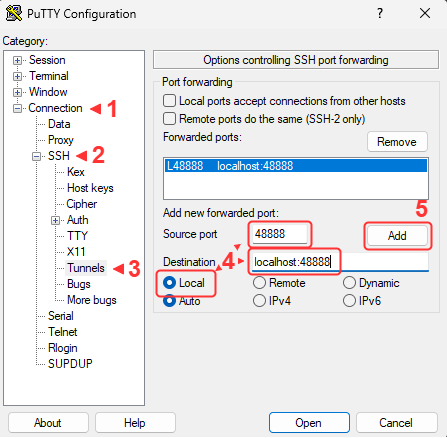
\includegraphics[keepaspectratio]{img/lab3/putty_port_forward.png}}

\subsubsection{Workspace}\label{workspace-1}

Let's create a new workspace for this lab.

\begin{Shaded}
\begin{Highlighting}[]
\BuiltInTok{cd}\NormalTok{ \textasciitilde{}/workspace}
\FunctionTok{mkdir}\NormalTok{ amb\_module4}
\BuiltInTok{cd}\NormalTok{ amb\_module4}
\end{Highlighting}
\end{Shaded}

Link the resource folder for easy access.

\begin{Shaded}
\begin{Highlighting}[]
\FunctionTok{ln} \AttributeTok{{-}s}\NormalTok{ \textasciitilde{}/CourseData/MIC\_data/amb\_module4/ ./lib}
\end{Highlighting}
\end{Shaded}

The expected outputs for this lab can be found in \texttt{./lib/outputs}.

\begin{Shaded}
\begin{Highlighting}[]
\FunctionTok{ls}\NormalTok{ ./lib/outputs}
\end{Highlighting}
\end{Shaded}

\subsubsection{Start container}\label{start-container-1}

Unpack the main container for this lab (\url{https://quay.io/repository/hallamlab/cbw_amb_lab4?tab=tags}).

\begin{Shaded}
\begin{Highlighting}[]
\ExtensionTok{apptainer}\NormalTok{ exec }\AttributeTok{{-}B}\NormalTok{ /media:/media ./lib/amb\_lab4.sif unpack}
\end{Highlighting}
\end{Shaded}

The following will dedicate the current terminal to running the juptyer notebook on port 48888.
You may want to connect another terminal to maintain terminal access.

\begin{Shaded}
\begin{Highlighting}[]
\ExtensionTok{./start\_lab}
\end{Highlighting}
\end{Shaded}

\subsubsection{Jupyter}\label{jupyter-1}

JupyterLab should now be accessible at \url{http://localhost:48888/lab}. Create a new python notebook and import dependencies.

\begin{Shaded}
\begin{Highlighting}[numbers=left,,]
\ImportTok{import}\NormalTok{ os}
\ImportTok{import}\NormalTok{ pandas }\ImportTok{as}\NormalTok{ pd}
\ImportTok{from}\NormalTok{ pathlib }\ImportTok{import}\NormalTok{ Path}

\NormalTok{LIB }\OperatorTok{=}\NormalTok{ Path(}\StringTok{"./lib"}\NormalTok{)}
\NormalTok{CPUS }\OperatorTok{=} \DecValTok{4} \CommentTok{\# your workshop instance has been alloted 4 cores}
\end{Highlighting}
\end{Shaded}

All software tools are packaged in the main container, so we can use \texttt{os.system("...")} instead of \texttt{Shell}.

\begin{Shaded}
\begin{Highlighting}[numbers=left,,]
\NormalTok{os.system(}\SpecialStringTok{f"""}
\SpecialStringTok{pwd {-}P}
\SpecialStringTok{echo }\SpecialCharTok{\{}\NormalTok{LIB}\SpecialCharTok{\}}
\SpecialStringTok{"""}\NormalTok{)}
\end{Highlighting}
\end{Shaded}

\subsection{Overview}\label{overview-2}

To understand the objective of this lab, let's first have a look at the metadata.

\begin{Shaded}
\begin{Highlighting}[numbers=left,,]
\NormalTok{df\_meta }\OperatorTok{=}\NormalTok{ pd.read\_csv(LIB}\OperatorTok{/}\StringTok{"inputs/metagenome\_metadata.txt"}\NormalTok{, sep}\OperatorTok{=}\StringTok{"}\CharTok{\textbackslash{}t}\StringTok{"}\NormalTok{)}
\BuiltInTok{print}\NormalTok{(df\_meta.shape)}
\NormalTok{df\_meta.head(}\DecValTok{2}\NormalTok{)}
\end{Highlighting}
\end{Shaded}

How many samples and how many categories?

We have 33 samples divided into ``Bacteroides'' and ``Non-Bacteroides'' groups.

We also have a set of predicted genes.

\begin{Shaded}
\begin{Highlighting}[numbers=left,,]
\ImportTok{from}\NormalTok{ Bio }\ImportTok{import}\NormalTok{ SeqIO}

\NormalTok{count }\OperatorTok{=} \DecValTok{0}
\NormalTok{genes\_fasta }\OperatorTok{=}\NormalTok{ LIB}\OperatorTok{/}\StringTok{"inputs/lab3\_orfs.fna"}
\ControlFlowTok{for}\NormalTok{ i, sequence }\KeywordTok{in} \BuiltInTok{enumerate}\NormalTok{(SeqIO.parse(genes\_fasta, }\StringTok{"fasta"}\NormalTok{)):}
\NormalTok{    count }\OperatorTok{+=} \DecValTok{1}
\NormalTok{count}
\end{Highlighting}
\end{Shaded}

The objective of this lab is to identify and visualize the pathways who's gene expression patterns correlate with the Bacteroides vs Non-Bacteroides grouping.
To do this we will:

\begin{enumerate}
\def\labelenumi{\arabic{enumi}.}
\tightlist
\item
  Use \hyperref[salmon]{salmon} to obtain a count matrix representing the expression level of each gene in each sample.
\item
  Use \hyperref[deseq2]{deseq2} to identify significantly expressed genes and generate a null distribution for gene set enrichment analysis.
\item
  Perform \hyperref[gene-set-enrichment-analysis-gsea]{Gene set enrichment analysis (GSEA)} to identify significantly enriched pathways.
\item
  Visualize the metabolic network in \hyperref[cytoscape]{cytoscape} with expression information.
\end{enumerate}

\subsection{Salmon}\label{salmon}

The alignment of transcriptomic reads to genes is often ambiguous. A single read can map to multiple genes and the length of genes compared to reads
means that multiple reads will map to different regions of the same gene. Salmon uses probabilistic and statistical models to quantify the expression of
each gene while also addressing potential biases {[}1{]}. We will use salmon to obtain a count matrix for deseq2.

\begin{enumerate}
\def\labelenumi{\arabic{enumi}.}
\tightlist
\item
  Patro R, Duggal G, Love MI, Irizarry RA, Kingsford C. Salmon provides fast and bias-aware quantification of transcript expression. Nat Methods. 2017;14(4):417--9. \url{https://doi.org/10.1038/nmeth.4197}
\end{enumerate}

Let's have a look at the help message.

\begin{Shaded}
\begin{Highlighting}[numbers=left,,]
\NormalTok{os.system(}\SpecialStringTok{f"salmon {-}{-}help"}\NormalTok{)}
\end{Highlighting}
\end{Shaded}

\begin{Shaded}
\begin{Highlighting}[numbers=left,,]
\NormalTok{os.system(}\SpecialStringTok{f"salmon index {-}{-}help"}\NormalTok{)}
\end{Highlighting}
\end{Shaded}

\begin{Shaded}
\begin{Highlighting}[numbers=left,,]
\NormalTok{os.system(}\SpecialStringTok{f"salmon quant {-}{-}help"}\NormalTok{)}
\end{Highlighting}
\end{Shaded}

We will need to index the reference genes before performing quantification.

\begin{Shaded}
\begin{Highlighting}[numbers=left,,]
\NormalTok{salmon\_dir }\OperatorTok{=}\NormalTok{ Path(}\StringTok{"./salmon"}\NormalTok{)}
\NormalTok{genes\_fasta }\OperatorTok{=}\NormalTok{ LIB}\OperatorTok{/}\StringTok{"inputs/lab3\_orfs.fna"}
\NormalTok{salmon\_index }\OperatorTok{=}\NormalTok{ salmon\_dir}\OperatorTok{/}\StringTok{"index"}
\NormalTok{os.system(}\SpecialStringTok{f"salmon index {-}t }\SpecialCharTok{\{}\NormalTok{genes\_fasta}\SpecialCharTok{\}}\SpecialStringTok{ {-}i }\SpecialCharTok{\{}\NormalTok{salmon\_index}\SpecialCharTok{\}}\SpecialStringTok{"}\NormalTok{)}
\end{Highlighting}
\end{Shaded}

We will quantify our samples. First, let's load them into a list.

\begin{Shaded}
\begin{Highlighting}[numbers=left,,]
\ImportTok{from}\NormalTok{ tqdm }\ImportTok{import}\NormalTok{ tqdm }\CommentTok{\# this draws progress bars for us}

\NormalTok{reads\_dir }\OperatorTok{=}\NormalTok{ LIB}\OperatorTok{/}\StringTok{"inputs/reads"}
\NormalTok{samples }\OperatorTok{=} \BuiltInTok{list}\NormalTok{(reads\_dir.iterdir())}
\end{Highlighting}
\end{Shaded}

\textbf{Quantification will take about 20 minutes. Do not run.}
Precomputed outputs are at \texttt{./lib/outputs/salmon/}.

\begin{Shaded}
\begin{Highlighting}[numbers=left,,]
\ControlFlowTok{for}\NormalTok{ read\_file }\KeywordTok{in}\NormalTok{ tqdm(samples, total}\OperatorTok{=}\BuiltInTok{len}\NormalTok{(samples)):}
\NormalTok{    srr }\OperatorTok{=}\NormalTok{ read\_file.name.split(}\StringTok{"\_"}\NormalTok{)[}\DecValTok{0}\NormalTok{]}
\NormalTok{    out }\OperatorTok{=}\NormalTok{ salmon\_dir}\OperatorTok{/}\SpecialStringTok{f"}\SpecialCharTok{\{}\NormalTok{srr}\SpecialCharTok{\}}\SpecialStringTok{"}
\NormalTok{    os.system(}\SpecialStringTok{f"""}
\SpecialStringTok{        mkdir {-}p }\SpecialCharTok{\{}\NormalTok{out}\SpecialCharTok{\}}
\SpecialStringTok{        salmon quant }\CharTok{\textbackslash{}}
\SpecialStringTok{            {-}l A }\CharTok{\textbackslash{}}
\SpecialStringTok{            {-}p }\SpecialCharTok{\{}\NormalTok{CPUS}\SpecialCharTok{\}}\SpecialStringTok{ }\CharTok{\textbackslash{}}
\SpecialStringTok{            {-}i }\SpecialCharTok{\{}\NormalTok{salmon\_index}\SpecialCharTok{\}}\SpecialStringTok{ }\CharTok{\textbackslash{}}
\SpecialStringTok{            {-}r }\SpecialCharTok{\{}\NormalTok{read\_file}\SpecialCharTok{\}}\SpecialStringTok{ }\CharTok{\textbackslash{}}
\SpecialStringTok{            {-}o }\SpecialCharTok{\{}\NormalTok{out}\SpecialCharTok{\}}\SpecialStringTok{ }\CharTok{\textbackslash{}}
\SpecialStringTok{            \textgreater{}}\SpecialCharTok{\{}\NormalTok{out}\SpecialCharTok{\}}\SpecialStringTok{/salmon.log 2\textgreater{}}\SpecialCharTok{\{}\NormalTok{out}\SpecialCharTok{\}}\SpecialStringTok{/salmon.err}
\SpecialStringTok{    """}\NormalTok{)}
\end{Highlighting}
\end{Shaded}

Salmon requires information about the reads' library type, such as stranded, unstranded, facing, paired-end, etc. \texttt{-l\ A} will tell Salmon to infer the type
from the first 1000 reads. \href{https://salmon.readthedocs.io/en/latest/salmon.html\#what-s-this-libtype}{More information is here.}

Let's have a look at one of the results. The file we want is \texttt{quant.sf}.

\begin{Shaded}
\begin{Highlighting}[numbers=left,,]
\NormalTok{salmon\_dir }\OperatorTok{=}\NormalTok{ LIB}\OperatorTok{/}\StringTok{"outputs/salmon/"} \CommentTok{\# divert}
\ControlFlowTok{for}\NormalTok{ srr }\KeywordTok{in}\NormalTok{ salmon\_dir.iterdir():}
    \ControlFlowTok{if} \KeywordTok{not}\NormalTok{ srr.name.startswith(}\StringTok{"SRR"}\NormalTok{): }\ControlFlowTok{continue}
\NormalTok{    df }\OperatorTok{=}\NormalTok{ pd.read\_csv(srr}\OperatorTok{/}\StringTok{"quant.sf"}\NormalTok{, sep}\OperatorTok{=}\StringTok{"}\CharTok{\textbackslash{}t}\StringTok{"}\NormalTok{)}
    \ControlFlowTok{break}
\NormalTok{df}
\end{Highlighting}
\end{Shaded}

The \texttt{TPM} (transcipts per million) column is useful on its own, but deseq2 prefers raw counts, so we will use the \texttt{NumReads} column.
Let's create the count matrix of genes by samples. First, create an index of genes.

\begin{Shaded}
\begin{Highlighting}[numbers=left,,]
\NormalTok{gene2i }\OperatorTok{=}\NormalTok{ \{\}}
\ControlFlowTok{for}\NormalTok{ i, sequence }\KeywordTok{in} \BuiltInTok{enumerate}\NormalTok{(SeqIO.parse(genes\_fasta, }\StringTok{"fasta"}\NormalTok{)):}
\NormalTok{    gene2i[sequence.}\BuiltInTok{id}\NormalTok{] }\OperatorTok{=}\NormalTok{ i}
\BuiltInTok{len}\NormalTok{(gene2i)}
\end{Highlighting}
\end{Shaded}

Now, we will load the counts for each sample into the matrix by matching the gene name using the index.

What are the expected dimensions of the count matrix?

Genes x Samples, so 3298 x 33.

\begin{center}\rule{0.5\linewidth}{0.5pt}\end{center}

\begin{Shaded}
\begin{Highlighting}[numbers=left,,]
\ImportTok{import}\NormalTok{ numpy }\ImportTok{as}\NormalTok{ np}

\NormalTok{mtx }\OperatorTok{=}\NormalTok{ np.zeros(shape}\OperatorTok{=}\NormalTok{(}\BuiltInTok{len}\NormalTok{(gene2i), }\BuiltInTok{len}\NormalTok{(samples)), dtype}\OperatorTok{=}\NormalTok{np.int32) }\CommentTok{\# genes x samples}
\ControlFlowTok{for}\NormalTok{ i, srr }\KeywordTok{in}\NormalTok{ tqdm(}\BuiltInTok{enumerate}\NormalTok{(df\_meta[}\StringTok{"sample\_name"}\NormalTok{]), total}\OperatorTok{=}\BuiltInTok{len}\NormalTok{(df\_meta)):}
\NormalTok{    df }\OperatorTok{=}\NormalTok{ pd.read\_csv(salmon\_dir}\OperatorTok{/}\SpecialStringTok{f"}\SpecialCharTok{\{}\NormalTok{srr}\SpecialCharTok{\}}\SpecialStringTok{/quant.sf"}\NormalTok{, sep}\OperatorTok{=}\StringTok{"}\CharTok{\textbackslash{}t}\StringTok{"}\NormalTok{)}

\NormalTok{    gene\_indexes }\OperatorTok{=}\NormalTok{ [gene2i[row[}\StringTok{"Name"}\NormalTok{]] }\ControlFlowTok{for}\NormalTok{ \_, row }\KeywordTok{in}\NormalTok{ df.iterrows()]}
\NormalTok{    counts }\OperatorTok{=}\NormalTok{ df[}\StringTok{"NumReads"}\NormalTok{]}
\NormalTok{    mtx[gene\_indexes, i] }\OperatorTok{=}\NormalTok{ counts}
\NormalTok{mtx.shape}
\end{Highlighting}
\end{Shaded}

Finally, we will label the rows and columns of the matrix with gene IDs and sample names before saving it to a file.

\begin{Shaded}
\begin{Highlighting}[numbers=left,,]
\NormalTok{gene\_ids }\OperatorTok{=} \BuiltInTok{list}\NormalTok{(gene2i.keys())}
\NormalTok{sample\_ids }\OperatorTok{=} \BuiltInTok{list}\NormalTok{(df\_meta[}\StringTok{"sample\_name"}\NormalTok{])}

\NormalTok{df }\OperatorTok{=}\NormalTok{ pd.DataFrame(mtx, columns}\OperatorTok{=}\NormalTok{sample\_ids)}
\NormalTok{df[}\StringTok{"gene\_id"}\NormalTok{] }\OperatorTok{=}\NormalTok{ gene\_ids}
\NormalTok{df }\OperatorTok{=}\NormalTok{ df.set\_index(}\StringTok{"gene\_id"}\NormalTok{)}
\BuiltInTok{print}\NormalTok{(df.shape)}
\NormalTok{df.to\_csv(}\StringTok{"./salmon/counts.mtx"}\NormalTok{)}
\NormalTok{df.head(}\DecValTok{2}\NormalTok{)}
\end{Highlighting}
\end{Shaded}

We are now ready for deseq2.

\subsection{DESeq2}\label{deseq2}

DESeq2 is a statistical package for R that is used to analyze count data from RNA-Seq experiments {[}1{]}.
It uses a negative binomial distribution to model count data, taking into account large biological diversity and technical noise
(overdispersion). We will use the statistical models and tools provided by DESeq2 to calculate fold changes and estimate significance.
The main purpose of DESeq2 in this lab is to generate the needed data for GSEA, which includes estimating the correlation between
gene expression and the experimental groups: Bacteroides and Non-Bacteroides. We will also generate a null distribution for
GSEA by permuting the sample labels.

\begin{enumerate}
\def\labelenumi{\arabic{enumi}.}
\tightlist
\item
  Patro R, Duggal G, Love MI, Irizarry RA, Kingsford C. Salmon provides fast and bias-aware quantification of transcript expression. Nat Methods. 2017;14(4):417--9. \url{https://doi.org/10.1038/nmeth.4197}
\end{enumerate}

\textbf{Transistion to an R notebook.} Click on the \texttt{+} and select ``R'' under Notebook.
\pandocbounded{
\includegraphics[keepaspectratio]{img/lab4/new_tab.png}}

\begin{Shaded}
\begin{Highlighting}[numbers=left,,]
\FunctionTok{library}\NormalTok{(DESeq2)}
\FunctionTok{library}\NormalTok{(readr)}
\end{Highlighting}
\end{Shaded}

load the count matrix

\begin{Shaded}
\begin{Highlighting}[numbers=left,,]
\NormalTok{cts }\OtherTok{\textless{}{-}} \FunctionTok{as.matrix}\NormalTok{(}\FunctionTok{read.csv}\NormalTok{(}
    \StringTok{"./salmon/counts.mtx"}\NormalTok{,}
    \AttributeTok{row.names =} \StringTok{"gene\_id"}
\NormalTok{))}
\NormalTok{cts}
\end{Highlighting}
\end{Shaded}

load the sample metadata

\begin{Shaded}
\begin{Highlighting}[numbers=left,,]
\NormalTok{coldata }\OtherTok{\textless{}{-}} \FunctionTok{read.csv}\NormalTok{(}
    \StringTok{"./lib/inputs/metagenome\_metadata.txt"}\NormalTok{,}
    \AttributeTok{sep =} \StringTok{"}\SpecialCharTok{\textbackslash{}t}\StringTok{"}\NormalTok{,}
\NormalTok{)}
\NormalTok{coldata}\SpecialCharTok{$}\NormalTok{grouping}
\end{Highlighting}
\end{Shaded}

Create a Deseq dataset object.

\begin{Shaded}
\begin{Highlighting}[numbers=left,,]
\NormalTok{dds }\OtherTok{\textless{}{-}} \FunctionTok{DESeqDataSetFromMatrix}\NormalTok{(}
  \AttributeTok{countData =}\NormalTok{ cts,}
  \AttributeTok{colData =}\NormalTok{ coldata,}
  \AttributeTok{design =} \SpecialCharTok{\textasciitilde{}}\NormalTok{ grouping}
\NormalTok{)}
\NormalTok{dds}
\end{Highlighting}
\end{Shaded}

This is how we would run DESeq2, but don't run it just yet.

\begin{Shaded}
\begin{Highlighting}[numbers=left,,]
\NormalTok{dds }\OtherTok{\textless{}{-}} \FunctionTok{DESeq}\NormalTok{(dds)}
\end{Highlighting}
\end{Shaded}

We can cache the results to an ``R data serialized'' (RDS) to prevent having to re-run this analysis when restarting the notebook.

\begin{Shaded}
\begin{Highlighting}[numbers=left,,]
\NormalTok{deseq\_save }\OtherTok{\textless{}{-}} \StringTok{"./deseq2/dds.rds"}
\ControlFlowTok{if}\NormalTok{ (}\SpecialCharTok{!}\FunctionTok{file.exists}\NormalTok{(deseq\_save)) \{}
\NormalTok{  dds }\OtherTok{\textless{}{-}} \FunctionTok{DESeq}\NormalTok{(dds)}
  \FunctionTok{dir.create}\NormalTok{(}\StringTok{"./deseq2"}\NormalTok{, }\AttributeTok{showWarnings =} \ConstantTok{TRUE}\NormalTok{) }\CommentTok{\# create the directory if it doesn\textquotesingle{}t exist}
  \FunctionTok{saveRDS}\NormalTok{(dds, deseq\_save)}
\NormalTok{\} }\ControlFlowTok{else}\NormalTok{ \{}
\NormalTok{  dds }\OtherTok{\textless{}{-}} \FunctionTok{readRDS}\NormalTok{(deseq\_save)}
\NormalTok{\}}
\end{Highlighting}
\end{Shaded}

Extract the results and save to a dataframe. This will contain log2 fold changes and p-values for each gene.

\begin{Shaded}
\begin{Highlighting}[numbers=left,,]
\NormalTok{res }\OtherTok{\textless{}{-}} \FunctionTok{results}\NormalTok{(dds, }\AttributeTok{contrast =} \FunctionTok{c}\NormalTok{(}\StringTok{"grouping"}\NormalTok{, }\StringTok{"Bacteroides"}\NormalTok{, }\StringTok{"Non{-}Bacteroides"}\NormalTok{))}
\NormalTok{results\_table }\OtherTok{\textless{}{-}} \FunctionTok{as.data.frame}\NormalTok{(res)}
\FunctionTok{write.csv}\NormalTok{(results\_table, }\StringTok{"./deseq2/results.csv"}\NormalTok{, }\AttributeTok{row.names =} \ConstantTok{TRUE}\NormalTok{)}
\NormalTok{results\_table}
\end{Highlighting}
\end{Shaded}

Next, we will compute the correlation between gene expression and the experimental groups and generate a null distribution for GSEA
by permuting the sample labels. This effectively randomizes the assignemnt of samples
to each experimental condition, but preserves any relationships between genes within a single sample.
When the number of samples is low, genes can be randomly assigned to gene sets instead, but this fails to take into account gene-gene relationships.
The p-value is estimated as the fraction of null samples that have a GSEA score greater than or equal to the observed GSEA score.

What is the minimum number of samples to simulate a null distribution with a precision of at least 0.05?

4 samples (4! = 24, 1/24 is about 0.04).

\begin{center}\rule{0.5\linewidth}{0.5pt}\end{center}

We will use the suggested variance stablized transform (VST) to obtain normalized counts. VST removes the dependence of variance on the mean,
which limits the high variance of the logarithm of counts when the mean is low.
(\href{https://bioconductor.org/packages/devel/bioc/vignettes/DESeq2/inst/doc/DESeq2.html\#:~:text=transformations\%20and\%20visualization-,Count\%20data\%20transformations,-In\%20order\%20to}{more info here}).

\begin{Shaded}
\begin{Highlighting}[numbers=left,,]
\NormalTok{vst }\OtherTok{\textless{}{-}} \FunctionTok{vst}\NormalTok{(dds, }\AttributeTok{blind =} \ConstantTok{FALSE}\NormalTok{)}
\NormalTok{vst\_counts }\OtherTok{\textless{}{-}} \FunctionTok{assay}\NormalTok{(vst)}
\NormalTok{vst\_counts}
\end{Highlighting}
\end{Shaded}

The human-readable class labels need to be converted to more machine-friendly ordinal labels.

\begin{Shaded}
\begin{Highlighting}[numbers=left,,]
\NormalTok{coldata}\SpecialCharTok{$}\NormalTok{grouping}
\NormalTok{class\_labels\_ordinal }\OtherTok{\textless{}{-}} \DecValTok{1} \SpecialCharTok{{-}}\NormalTok{ (}\FunctionTok{as.numeric}\NormalTok{(}\FunctionTok{factor}\NormalTok{(coldata}\SpecialCharTok{$}\NormalTok{grouping)) }\SpecialCharTok{{-}} \DecValTok{1}\NormalTok{)}
\NormalTok{class\_labels\_ordinal}
\end{Highlighting}
\end{Shaded}

We will use the point biserial correlation, a special case of the Pearson correlation designed to compare a continuous variable with a binary variable.
Alternatively the biserial correlation achieves nearly the same, but assumes that the binary variable is the result of thresholding a continuous variable.
For example, it would be appropriate to use the point biserial correlation for a coin toss, while the biserial correlation would be more appropriate for pass/fails from percentage grades.
Practically, the biserial correlation also requires the relative propotions of each class. While there likely is a genetic spectrum of bacteria spanning
from Bacteroides to Non-Bacteroides, we don't have any information on this spectrum or the genetic threshold at which an organism stops being a Bacteroides.

\begin{Shaded}
\begin{Highlighting}[numbers=left,,]
\NormalTok{point\_biserial }\OtherTok{\textless{}{-}} \ControlFlowTok{function}\NormalTok{(expression, classes) \{}
  \ControlFlowTok{if}\NormalTok{ (}\FunctionTok{sd}\NormalTok{(expression) }\SpecialCharTok{==} \DecValTok{0}\NormalTok{) }\FunctionTok{return}\NormalTok{(}\ConstantTok{NA}\NormalTok{)}
  \FunctionTok{return}\NormalTok{(}\FunctionTok{cor}\NormalTok{(expression, classes, }\AttributeTok{method =} \StringTok{"pearson"}\NormalTok{))}
\NormalTok{\}}
\end{Highlighting}
\end{Shaded}

Estimate the observed correlation.

\begin{Shaded}
\begin{Highlighting}[numbers=left,,]
\NormalTok{gene\_correlations }\OtherTok{\textless{}{-}} \FunctionTok{apply}\NormalTok{(vst\_counts, }\DecValTok{1}\NormalTok{, point\_biserial, }\AttributeTok{classes =}\NormalTok{ class\_labels\_ordinal)}
\NormalTok{gene\_correlations }\OtherTok{\textless{}{-}} \FunctionTok{as.data.frame}\NormalTok{(gene\_correlations)}
\FunctionTok{write.csv}\NormalTok{(gene\_correlations, }\StringTok{"./deseq2/gene\_correlations.csv"}\NormalTok{, }\AttributeTok{row.names =} \ConstantTok{TRUE}\NormalTok{)}
\end{Highlighting}
\end{Shaded}

To generate the null distribution, we will be taking many samples (200). The following libraries will enable us to parallelize the computation.

\begin{Shaded}
\begin{Highlighting}[numbers=left,,]
\FunctionTok{library}\NormalTok{(pbapply)}
\FunctionTok{library}\NormalTok{(parallel)}
\end{Highlighting}
\end{Shaded}

Since this is computationally expensive, we will use the caching technique shown earlier.

\begin{Shaded}
\begin{Highlighting}[numbers=left,,]
\NormalTok{null\_save }\OtherTok{\textless{}{-}} \StringTok{"./deseq2/null\_distr.csv"}

\ControlFlowTok{if}\NormalTok{ (}\SpecialCharTok{!}\FunctionTok{file.exists}\NormalTok{(null\_save)) \{}

  \FunctionTok{tryCatch}\NormalTok{(             }\CommentTok{\# if anything goes wrong, we must run the "finally" block}
\NormalTok{    \{}
\NormalTok{      cl }\OtherTok{\textless{}{-}} \FunctionTok{makeCluster}\NormalTok{(}\DecValTok{4}\NormalTok{) }\CommentTok{\# make a cluster with 4 workers}
      \CommentTok{\# make these variables available to each worker}
      \FunctionTok{clusterExport}\NormalTok{(cl, }\FunctionTok{c}\NormalTok{(}\StringTok{"vst\_counts"}\NormalTok{, }\StringTok{"point\_biserial"}\NormalTok{, }\StringTok{"class\_labels\_ordinal"}\NormalTok{))}

\NormalTok{      n\_permutations }\OtherTok{\textless{}{-}} \DecValTok{200}
\NormalTok{      permutation\_results }\OtherTok{\textless{}{-}} \FunctionTok{pbsapply}\NormalTok{(}
        \DecValTok{1}\SpecialCharTok{:}\NormalTok{n\_permutations,   }\CommentTok{\# iterate 200 times}
        \ControlFlowTok{function}\NormalTok{(i) \{       }\CommentTok{\# and run this function each time}
          \CommentTok{\# Shuffle labels}
\NormalTok{          n }\OtherTok{\textless{}{-}} \FunctionTok{length}\NormalTok{(class\_labels\_ordinal)}
\NormalTok{          shuffled\_labels }\OtherTok{\textless{}{-}} \FunctionTok{sample}\NormalTok{(class\_labels\_ordinal, }\AttributeTok{size =}\NormalTok{ n, }\AttributeTok{replace =} \ConstantTok{FALSE}\NormalTok{)}

          \CommentTok{\# Calculate correlations for all genes}
          \FunctionTok{return}\NormalTok{(}\FunctionTok{apply}\NormalTok{(vst\_counts, }\DecValTok{1}\NormalTok{, point\_biserial, }\AttributeTok{classes =}\NormalTok{ shuffled\_labels))}
\NormalTok{        \},}
        \AttributeTok{cl =}\NormalTok{ cl }\CommentTok{\# use workers to compute in parallel}
\NormalTok{      )}
\NormalTok{    \},}
    \AttributeTok{finally =}\NormalTok{ \{         }\CommentTok{\# no matter what happens}
      \FunctionTok{stopCluster}\NormalTok{(cl)   }\CommentTok{\# remember to stop the cluster}
\NormalTok{    \}}
\NormalTok{  )}

  \CommentTok{\# cache results as a dataframe}
\NormalTok{  null\_distr }\OtherTok{\textless{}{-}} \FunctionTok{data.frame}\NormalTok{(}
    \AttributeTok{sample =}\NormalTok{ permutation\_results,}
    \AttributeTok{stringsAsFactors =} \ConstantTok{FALSE}
\NormalTok{  )}
  \FunctionTok{write.csv}\NormalTok{(}
\NormalTok{    null\_distr,}
\NormalTok{    null\_save,}
    \AttributeTok{row.names =} \ConstantTok{TRUE}
\NormalTok{  )}
\NormalTok{\} }\ControlFlowTok{else}\NormalTok{ \{}
\NormalTok{  null\_distr }\OtherTok{\textless{}{-}} \FunctionTok{read.csv}\NormalTok{(null\_save)}
\NormalTok{\}}

\FunctionTok{dim}\NormalTok{(null\_distr)}
\end{Highlighting}
\end{Shaded}

\subsection{Gene set enrichment analysis (GSEA)}\label{gene-set-enrichment-analysis-gsea}

\textbf{Back to python.}

GSEA ranks genes by their correlation with experimental groups, then examines the overrepresentation of gene sets in highly ranked genes by calculating an
enrichment score (ES) {[}1{]}. The observed ES compared to the null distribution of enrichment scores is then used to estimate the significance of the observed ES.
To apply GSEA, we need:

\begin{itemize}
\tightlist
\item
  N samples where M continuous features are measured (eg. N transcriptomic samples for M genes, N metagenomes of M members, N pictures of M pixels, etc.)
\item
  Groupings (overlap permitted) of these M features to test
\end{itemize}

Despite GSEA being widely applicable, implementations are overly specific to human transcriptomics, rendering them difficult to adapt to even adjacent domains.
Fortunately, the technique itself is rather straightforward to implement.

\begin{enumerate}
\def\labelenumi{\arabic{enumi}.}
\tightlist
\item
  Patro R, Duggal G, Love MI, Irizarry RA, Kingsford C. Salmon provides fast and bias-aware quantification of transcript expression. Nat Methods. 2017;14(4):417--9. \url{https://doi.org/10.1038/nmeth.4197}
\end{enumerate}

We will use KEGG pathways as our gene sets. These were predicted using Kofamscan from the previous lab.

\begin{Shaded}
\begin{Highlighting}[numbers=left,,]
\ImportTok{from}\NormalTok{ local.models.kegg\_orthology }\ImportTok{import}\NormalTok{ ParseKofamScanResults}

\NormalTok{kegg\_model }\OperatorTok{=}\NormalTok{ ParseKofamScanResults(}
\NormalTok{    LIB}\OperatorTok{/}\StringTok{"inputs/kofamscan/kos.out"}\NormalTok{,}
\NormalTok{    LIB}\OperatorTok{/}\StringTok{"kofamscan\_db/api\_kegg.db"}\NormalTok{,}
\NormalTok{    LIB}\OperatorTok{/}\StringTok{"kofamscan\_db/brite.json"}\NormalTok{,}
\NormalTok{)}
\end{Highlighting}
\end{Shaded}

We will find the pathways for each gene by tracing: \texttt{gene\ -\textgreater{}\ function\ -\textgreater{}\ reaction\ -\textgreater{}\ pathway}.

\begin{Shaded}
\begin{Highlighting}[numbers=left,,]
\NormalTok{function2genes }\OperatorTok{=}\NormalTok{ \{\}}
\ControlFlowTok{for}\NormalTok{ \_, r }\KeywordTok{in}\NormalTok{ kegg\_model.df.iterrows():}
\NormalTok{    ko }\OperatorTok{=}\NormalTok{ r[}\StringTok{"ko"}\NormalTok{]}
\NormalTok{    orf }\OperatorTok{=}\NormalTok{ r[}\StringTok{"orf"}\NormalTok{]}
\NormalTok{    function2genes[ko] }\OperatorTok{=}\NormalTok{ function2genes.get(ko, }\BuiltInTok{set}\NormalTok{())}\OperatorTok{|}\NormalTok{\{orf\}}

\NormalTok{reactions2functions }\OperatorTok{=}\NormalTok{ \{\}}
\ControlFlowTok{for}\NormalTok{ ko }\KeywordTok{in}\NormalTok{ function2genes:}
\NormalTok{    meta }\OperatorTok{=}\NormalTok{ kegg\_model.Functions[ko]}
    \ControlFlowTok{for}\NormalTok{ r }\KeywordTok{in}\NormalTok{ meta.reactions:}
\NormalTok{        reactions2functions[r] }\OperatorTok{=}\NormalTok{ reactions2functions.get(r, }\BuiltInTok{set}\NormalTok{())}\OperatorTok{|}\NormalTok{\{ko\}}

\NormalTok{pathway2reactions }\OperatorTok{=}\NormalTok{ \{\}}
\ControlFlowTok{for}\NormalTok{ r }\KeywordTok{in}\NormalTok{ reactions2functions:}
\NormalTok{    meta }\OperatorTok{=}\NormalTok{ kegg\_model.Reactions[r]}
    \ControlFlowTok{for}\NormalTok{ p }\KeywordTok{in}\NormalTok{ meta.pathways:}
\NormalTok{        pathway2reactions[p] }\OperatorTok{=}\NormalTok{ pathway2reactions.get(p, }\BuiltInTok{set}\NormalTok{())}\OperatorTok{|}\NormalTok{\{r\}}

\NormalTok{gene\_sets }\OperatorTok{=}\NormalTok{ \{\} }\CommentTok{\# collect the genes for each pathway}
\ControlFlowTok{for}\NormalTok{ p, reactions }\KeywordTok{in}\NormalTok{ pathway2reactions.items():}
\NormalTok{    genes }\OperatorTok{=} \BuiltInTok{set}\NormalTok{()}
    \ControlFlowTok{for}\NormalTok{ r }\KeywordTok{in}\NormalTok{ reactions:}
\NormalTok{        functions }\OperatorTok{=}\NormalTok{ reactions2functions[r]}
        \ControlFlowTok{for}\NormalTok{ f }\KeywordTok{in}\NormalTok{ functions:}
\NormalTok{            genes }\OperatorTok{|=}\NormalTok{ function2genes[f]}
\NormalTok{    gene\_sets[p] }\OperatorTok{=}\NormalTok{ genes}
\end{Highlighting}
\end{Shaded}

Load correlations from DESeq2.

\begin{Shaded}
\begin{Highlighting}[numbers=left,,]
\NormalTok{deseq\_dir }\OperatorTok{=}\NormalTok{ Path(}\StringTok{"./deseq2"}\NormalTok{)}
\NormalTok{df\_null }\OperatorTok{=}\NormalTok{ pd.read\_csv(deseq\_dir}\OperatorTok{/}\StringTok{"null\_distr.csv"}\NormalTok{, index\_col}\OperatorTok{=}\DecValTok{0}\NormalTok{)}
\BuiltInTok{print}\NormalTok{(df\_null.shape)}
\NormalTok{df\_null.head(}\DecValTok{2}\NormalTok{)}
\end{Highlighting}
\end{Shaded}

\begin{Shaded}
\begin{Highlighting}[numbers=left,,]
\NormalTok{df\_corr }\OperatorTok{=}\NormalTok{ pd.read\_csv(deseq\_dir}\OperatorTok{/}\StringTok{"gene\_correlations.csv"}\NormalTok{, index\_col}\OperatorTok{=}\DecValTok{0}\NormalTok{)}
\BuiltInTok{print}\NormalTok{(df\_corr.shape)}
\NormalTok{df\_corr.head(}\DecValTok{2}\NormalTok{)}
\end{Highlighting}
\end{Shaded}

Next we will calculate the ES and p-value for an example pathway \texttt{rn00983}.

\begin{Shaded}
\begin{Highlighting}[numbers=left,,]
\NormalTok{gene\_set }\OperatorTok{=}\NormalTok{ gene\_sets[}\StringTok{"rn00983"}\NormalTok{]}
\NormalTok{kegg\_model.Pathways[}\StringTok{"rn00983"}\NormalTok{].name}
\end{Highlighting}
\end{Shaded}

First, create a matrix of permutations x genes, only taking those that are in gene sets.

\begin{Shaded}
\begin{Highlighting}[numbers=left,,]
\NormalTok{enzymes }\OperatorTok{=}\NormalTok{ \{x }\ControlFlowTok{for}\NormalTok{ g }\KeywordTok{in}\NormalTok{ gene\_sets.values() }\ControlFlowTok{for}\NormalTok{ x }\KeywordTok{in}\NormalTok{ g\}}
\KeywordTok{def}\NormalTok{ \_only\_enzymes(df: pd.DataFrame):}
    \ControlFlowTok{return}\NormalTok{ df.loc[df.index.isin(enzymes)]}

\NormalTok{corr }\OperatorTok{=}\NormalTok{ \_only\_enzymes(df\_corr).to\_numpy()}
\NormalTok{permuted }\OperatorTok{=}\NormalTok{ \_only\_enzymes(df\_null).to\_numpy()}
\NormalTok{mat }\OperatorTok{=}\NormalTok{ np.hstack([corr, permuted]) }\CommentTok{\# true correlations is the first permutation}
\NormalTok{mat.shape}
\end{Highlighting}
\end{Shaded}

Rank order the genes in each permutation by their correlation.

\begin{Shaded}
\begin{Highlighting}[numbers=left,,]
\NormalTok{mat\_index }\OperatorTok{=}\NormalTok{ np.argsort(}\OperatorTok{{-}}\NormalTok{mat.T, stable}\OperatorTok{=}\VariableTok{True}\NormalTok{)}
\NormalTok{mat\_sorted }\OperatorTok{=}\NormalTok{ np.zeros\_like(mat)}
\ControlFlowTok{for}\NormalTok{ i, order }\KeywordTok{in} \BuiltInTok{enumerate}\NormalTok{(mat\_index):}
\NormalTok{    mat\_sorted[:, i] }\OperatorTok{=}\NormalTok{ mat[:, i][order]}
\NormalTok{mat\_sorted.shape}
\end{Highlighting}
\end{Shaded}

Let's make a human-readable list of genes so we know what each position of the matrix corresponds to.
Notice how the length of labels corresponds to the genes axis of the matrix.

\begin{Shaded}
\begin{Highlighting}[numbers=left,,]
\NormalTok{labels }\OperatorTok{=}\NormalTok{ \_only\_enzymes(df\_corr).index.to\_numpy()}
\BuiltInTok{len}\NormalTok{(labels)}
\end{Highlighting}
\end{Shaded}

\subsubsection{(Optional: implementing GSEA)}\label{optional-implementing-gsea}

This section dives deep into python to implement GSEA from scratch.
It is often sufficient to use existing software, but especially new or domain specific algorithms may be more difficult to install
than implementing from scratch. Sometimes installation or implementation are both difficult\ldots{}
Our ultimate goal is to create this plot from figure 1 of the GSEA paper {[}1{]}

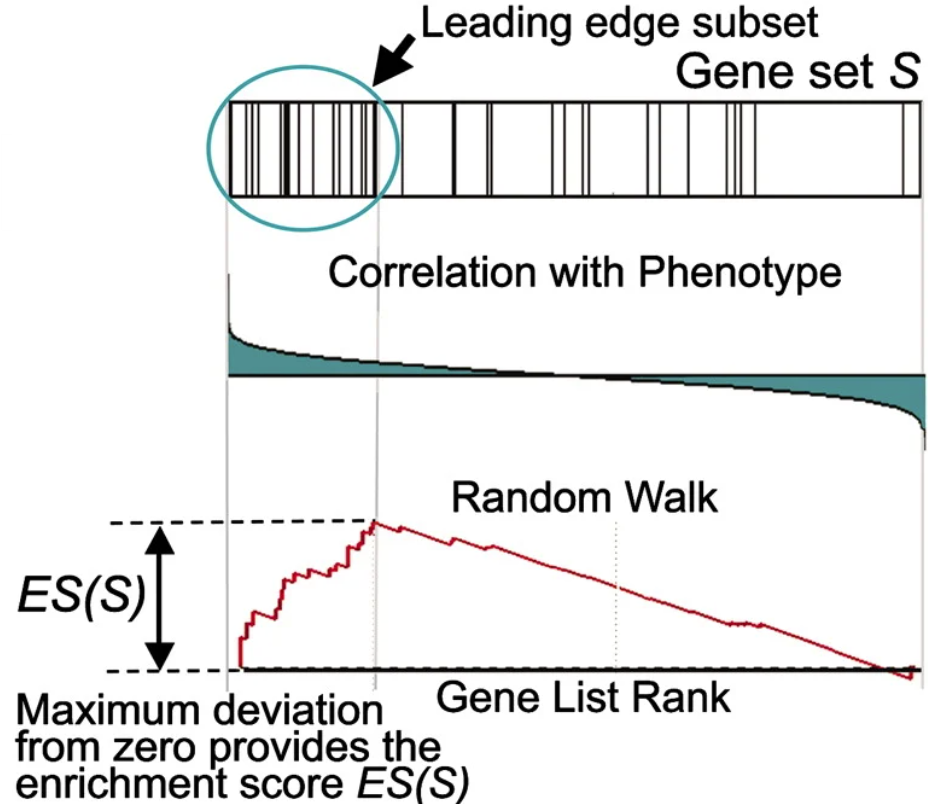
\includegraphics[width=0.5\linewidth,height=\textheight,keepaspectratio]{img/lab4/gsea.png}

To calculate the ES, a running sum is calculated by scanning down the ranked list of genes, increasing the score for genes that
are in the gene set and decreasing it otherwise. Genes in the gene set are called ``hits'' and those not in the gene set are called ``misses''.
The magnitude of the increase is dependent on the correlation between the gene
expression and the experimental grouping. The ES is the maximum deviation from 0 of this running sum statistic, caused by the commulative effect
of the genes ranked before the maximum deviation is reached (``leading edge subset'').

The running sum statistic is calculated as the difference between the effect of hits and misses.
The equation for the running sum of hits (P\_hit) at rank \emph{i}
for gene set \emph{S} is given in the paper. Don't look at all of it at once, we will break it down.
First, note that the summations only consider genes in the gene set \emph{S}.

\pandocbounded{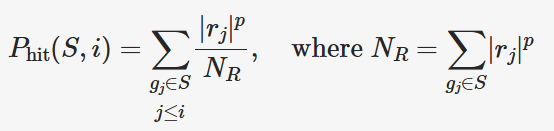
\includegraphics[keepaspectratio]{img/lab4/gsea_phit.png}}

Let's create a mask to select only genes in \emph{S}.

\begin{Shaded}
\begin{Highlighting}[numbers=left,,]
\NormalTok{S }\OperatorTok{=}\NormalTok{ np.array([k }\KeywordTok{in}\NormalTok{ gene\_set }\ControlFlowTok{for}\NormalTok{ k }\KeywordTok{in}\NormalTok{ labels], dtype}\OperatorTok{=}\BuiltInTok{int}\NormalTok{) }\CommentTok{\# g in S}
\NormalTok{S }\OperatorTok{=}\NormalTok{ S[mat\_index.T] }\CommentTok{\# same order as mat}
\end{Highlighting}
\end{Shaded}

Next, have a look at NR. rj is simply the correlation values of each gene. \emph{p} is a hyperparamter set to 1.
Let's calculate NR.

\begin{Shaded}
\begin{Highlighting}[numbers=left,,]
\NormalTok{p }\OperatorTok{=} \DecValTok{1}
\NormalTok{corr }\OperatorTok{=}\NormalTok{ np.}\BuiltInTok{pow}\NormalTok{(np.}\BuiltInTok{abs}\NormalTok{(mat\_sorted), p)}
\NormalTok{N\_R }\OperatorTok{=}\NormalTok{ np.}\BuiltInTok{sum}\NormalTok{(corr}\OperatorTok{*}\NormalTok{S, axis}\OperatorTok{=}\DecValTok{0}\NormalTok{)}
\end{Highlighting}
\end{Shaded}

We now need to combine the repeated \textbar rj\textbar{}p term in the numerator with
NR in the denominator and cumulatively sum up to each gene. \texttt{np.cumsum()} does this for us.

\begin{Shaded}
\begin{Highlighting}[numbers=left,,]
\NormalTok{P\_hit }\OperatorTok{=}\NormalTok{ corr}\OperatorTok{/}\NormalTok{N\_R}
\NormalTok{P\_hit }\OperatorTok{=}\NormalTok{ P\_hit}\OperatorTok{*}\NormalTok{S }\CommentTok{\# g\_j in S}
\NormalTok{P\_hit }\OperatorTok{=}\NormalTok{ np.cumsum(P\_hit, axis}\OperatorTok{=}\DecValTok{0}\NormalTok{)}
\end{Highlighting}
\end{Shaded}

Have a look.

\begin{Shaded}
\begin{Highlighting}[numbers=left,,]
\ImportTok{from}\NormalTok{ local.figures.template }\ImportTok{import}\NormalTok{ BaseFigure, ApplyTemplate, go}
\NormalTok{fig }\OperatorTok{=}\NormalTok{ BaseFigure()}
\NormalTok{fig.add\_trace(go.Scatter(}
\NormalTok{    x }\OperatorTok{=}\NormalTok{ np.arange(}\BuiltInTok{len}\NormalTok{(P\_hit[:, }\DecValTok{0}\NormalTok{])),}
\NormalTok{    y }\OperatorTok{=}\NormalTok{ P\_hit[:, }\DecValTok{0}\NormalTok{],}
\NormalTok{))}
\NormalTok{fig }\OperatorTok{=}\NormalTok{ ApplyTemplate(fig)}
\NormalTok{fig.show()}
\end{Highlighting}
\end{Shaded}

For P\_miss, we cumulatively sum the fraction of misses.

\pandocbounded{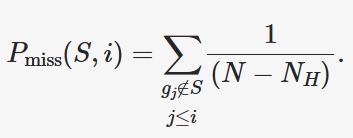
\includegraphics[keepaspectratio]{img/lab4/gsea_pmiss.png}}

\begin{Shaded}
\begin{Highlighting}[numbers=left,,]
\NormalTok{P\_miss }\OperatorTok{=} \DecValTok{1}\OperatorTok{/}\NormalTok{(}\BuiltInTok{len}\NormalTok{(labels) }\OperatorTok{{-}} \BuiltInTok{len}\NormalTok{(gene\_set))}
\NormalTok{\_mask }\OperatorTok{=} \DecValTok{1}\OperatorTok{{-}}\NormalTok{S.T }\CommentTok{\# invert hits for misses}
\NormalTok{P\_miss }\OperatorTok{=}\NormalTok{ np.ones\_like(labels)}\OperatorTok{*}\NormalTok{\_mask}\OperatorTok{*}\NormalTok{P\_miss}
\NormalTok{P\_miss }\OperatorTok{=}\NormalTok{ np.cumsum(P\_miss.T, axis}\OperatorTok{=}\DecValTok{0}\NormalTok{)}
\end{Highlighting}
\end{Shaded}

That's it, have a look.

\begin{Shaded}
\begin{Highlighting}[numbers=left,,]
\NormalTok{fig }\OperatorTok{=}\NormalTok{ BaseFigure()}
\NormalTok{fig.add\_trace(go.Scatter(}
\NormalTok{    x }\OperatorTok{=}\NormalTok{ np.arange(}\BuiltInTok{len}\NormalTok{(P\_miss[:, }\DecValTok{0}\NormalTok{])),}
\NormalTok{    y }\OperatorTok{=} \OperatorTok{{-}}\NormalTok{P\_miss[:, }\DecValTok{0}\NormalTok{],}
\NormalTok{))}
\NormalTok{fig }\OperatorTok{=}\NormalTok{ ApplyTemplate(fig)}
\NormalTok{fig.show()}
\end{Highlighting}
\end{Shaded}

Now we combine P\_hit and P\_miss to get the running sum statistic
and find the maximum magnitude to report the enrichment score (ES).

\begin{Shaded}
\begin{Highlighting}[numbers=left,,]
\NormalTok{S\_distr }\OperatorTok{=}\NormalTok{ (P\_hit }\OperatorTok{{-}}\NormalTok{ P\_miss).T }\CommentTok{\# running statistic}
\NormalTok{ES\_pos }\OperatorTok{=}\NormalTok{ S\_distr.}\BuiltInTok{max}\NormalTok{(axis}\OperatorTok{=}\DecValTok{1}\NormalTok{)}
\NormalTok{ES\_neg }\OperatorTok{=}\NormalTok{ S\_distr.}\BuiltInTok{min}\NormalTok{(axis}\OperatorTok{=}\DecValTok{1}\NormalTok{)}
\NormalTok{ES\_candidates }\OperatorTok{=}\NormalTok{ np.vstack([ES\_pos, ES\_neg]).T       }\CommentTok{\# candidate is either the positive or negative}
\NormalTok{to\_take }\OperatorTok{=}\NormalTok{ np.argmax(np.}\BuiltInTok{abs}\NormalTok{(ES\_candidates), axis}\OperatorTok{=}\DecValTok{1}\NormalTok{)  }\CommentTok{\# we must select for each permutation}
\NormalTok{ES }\OperatorTok{=}\NormalTok{ (ES\_neg}\OperatorTok{*}\NormalTok{to\_take) }\OperatorTok{+}\NormalTok{ (ES\_pos}\OperatorTok{*}\NormalTok{(}\DecValTok{1}\OperatorTok{{-}}\NormalTok{to\_take))}
\end{Highlighting}
\end{Shaded}

Have a look.

\begin{Shaded}
\begin{Highlighting}[numbers=left,,]
\NormalTok{fig }\OperatorTok{=}\NormalTok{ BaseFigure()}
\NormalTok{fig.add\_trace(go.Scatter(}
\NormalTok{    x }\OperatorTok{=}\NormalTok{ np.arange(}\BuiltInTok{len}\NormalTok{(S\_distr[}\DecValTok{0}\NormalTok{])),}
\NormalTok{    y }\OperatorTok{=}\NormalTok{ S\_distr[}\DecValTok{0}\NormalTok{],}
\NormalTok{))}
\NormalTok{fig }\OperatorTok{=}\NormalTok{ ApplyTemplate(fig)}
\NormalTok{fig.show()}
\end{Highlighting}
\end{Shaded}

We can now split the score and null distribution and estimate the p-value.

\begin{Shaded}
\begin{Highlighting}[numbers=left,,]
\NormalTok{score, null }\OperatorTok{=}\NormalTok{ ES[}\DecValTok{0}\NormalTok{], ES[}\DecValTok{1}\NormalTok{:]}
\NormalTok{pvalue }\OperatorTok{=}\NormalTok{ np.}\BuiltInTok{sum}\NormalTok{(null }\OperatorTok{\textgreater{}=}\NormalTok{ score) }\OperatorTok{/}\NormalTok{ null.shape[}\DecValTok{0}\NormalTok{]}
\ControlFlowTok{if}\NormalTok{ pvalue }\OperatorTok{==} \DecValTok{0}\NormalTok{:}
\NormalTok{    pvalue }\OperatorTok{=} \DecValTok{1} \OperatorTok{/}\NormalTok{ null.shape[}\DecValTok{0}\NormalTok{]}
\NormalTok{score, pvalue}
\end{Highlighting}
\end{Shaded}

Why do we change the pvalue if it is equal to 0?

If the p-value is 0, then the resolution of the null distribution was insufficient. To be conservative, we set it to the
smallest pvalue that is resolvable, which is 1/(the sample size of the null distribution).

Let's clean things up a bit. We will encapsulate the procedure in a function and
return a \texttt{dataclass}, which is just a convient way to organize a collection of variables.
We will use this function to run GSEA for each pathway. Try completing the \texttt{gsea()} function below.

\begin{Shaded}
\begin{Highlighting}[numbers=left,,]
\ImportTok{from}\NormalTok{ dataclasses }\ImportTok{import}\NormalTok{ dataclass}

\AttributeTok{@dataclass}
\KeywordTok{class}\NormalTok{ GseaResult:}
\NormalTok{    set\_name: }\BuiltInTok{str}
\NormalTok{    set\_size: }\BuiltInTok{int}
\NormalTok{    score: }\BuiltInTok{float}
\NormalTok{    pvalue: }\BuiltInTok{float}
\NormalTok{    hits: np.ndarray}
\NormalTok{    running\_sum\_statistic: np.ndarray}
    
\KeywordTok{def}\NormalTok{ gsea(name):}
\NormalTok{    gene\_set }\OperatorTok{=}\NormalTok{ gene\_sets[name]}
    
    \CommentTok{\# ...}

    \ControlFlowTok{return}\NormalTok{ GseaResult(}
\NormalTok{        set\_name}\OperatorTok{=}\NormalTok{name,}
\NormalTok{        set\_size}\OperatorTok{=}\BuiltInTok{len}\NormalTok{(gene\_set),}
\NormalTok{        score}\OperatorTok{=}\NormalTok{score,}
\NormalTok{        pvalue}\OperatorTok{=}\NormalTok{pvalue,}
\NormalTok{        hits}\OperatorTok{=}\NormalTok{S.T[}\DecValTok{0}\NormalTok{],}
\NormalTok{        running\_sum\_statistic}\OperatorTok{=}\NormalTok{S\_distr[}\DecValTok{0}\NormalTok{],}
\NormalTok{    )}

\NormalTok{res }\OperatorTok{=}\NormalTok{ gsea(}\StringTok{"rn00983"}\NormalTok{)}
\NormalTok{res.score, res.pvalue}
\end{Highlighting}
\end{Shaded}

\subsubsection{Running GSEA}\label{running-gsea}

Solution

\begin{Shaded}
\begin{Highlighting}[numbers=left,,]
\ImportTok{from}\NormalTok{ dataclasses }\ImportTok{import}\NormalTok{ dataclass}

\AttributeTok{@dataclass}
\KeywordTok{class}\NormalTok{ GseaResult:}
\NormalTok{    set\_name: }\BuiltInTok{str}
\NormalTok{    set\_size: }\BuiltInTok{int}
\NormalTok{    score: }\BuiltInTok{float}
\NormalTok{    pvalue: }\BuiltInTok{float}
\NormalTok{    hits: np.ndarray}
\NormalTok{    running\_sum\_statistic: np.ndarray}
    
\KeywordTok{def}\NormalTok{ gsea(name):}
\NormalTok{    gene\_set }\OperatorTok{=}\NormalTok{ gene\_sets[name]}
\NormalTok{    S }\OperatorTok{=}\NormalTok{ np.array([k }\KeywordTok{in}\NormalTok{ gene\_set }\ControlFlowTok{for}\NormalTok{ k }\KeywordTok{in}\NormalTok{ labels], dtype}\OperatorTok{=}\BuiltInTok{int}\NormalTok{) }\CommentTok{\# g in S}
\NormalTok{    S }\OperatorTok{=}\NormalTok{ S[mat\_index.T] }\CommentTok{\# same order as mat}

\NormalTok{    p }\OperatorTok{=} \DecValTok{1}
\NormalTok{    corr }\OperatorTok{=}\NormalTok{ np.}\BuiltInTok{pow}\NormalTok{(np.}\BuiltInTok{abs}\NormalTok{(mat\_sorted), p)}
\NormalTok{    N\_R }\OperatorTok{=}\NormalTok{ np.}\BuiltInTok{sum}\NormalTok{(corr}\OperatorTok{*}\NormalTok{S, axis}\OperatorTok{=}\DecValTok{0}\NormalTok{)}

\NormalTok{    P\_hit }\OperatorTok{=}\NormalTok{ corr}\OperatorTok{/}\NormalTok{N\_R}
\NormalTok{    P\_hit }\OperatorTok{=}\NormalTok{ P\_hit}\OperatorTok{*}\NormalTok{S }\CommentTok{\# g\_j in S}
\NormalTok{    P\_hit }\OperatorTok{=}\NormalTok{ np.cumsum(P\_hit, axis}\OperatorTok{=}\DecValTok{0}\NormalTok{)}

\NormalTok{    P\_miss }\OperatorTok{=} \DecValTok{1}\OperatorTok{/}\NormalTok{(}\BuiltInTok{len}\NormalTok{(labels) }\OperatorTok{{-}} \BuiltInTok{len}\NormalTok{(gene\_set))}
\NormalTok{    \_mask }\OperatorTok{=} \DecValTok{1}\OperatorTok{{-}}\NormalTok{S.T }\CommentTok{\# invert hits for misses}
\NormalTok{    P\_miss }\OperatorTok{=}\NormalTok{ np.ones\_like(labels)}\OperatorTok{*}\NormalTok{\_mask}\OperatorTok{*}\NormalTok{P\_miss}
\NormalTok{    P\_miss }\OperatorTok{=}\NormalTok{ np.cumsum(P\_miss.T, axis}\OperatorTok{=}\DecValTok{0}\NormalTok{)}

\NormalTok{    S\_distr }\OperatorTok{=}\NormalTok{ (P\_hit }\OperatorTok{{-}}\NormalTok{ P\_miss).T }\CommentTok{\# running statistic}
\NormalTok{    ES\_pos }\OperatorTok{=}\NormalTok{ S\_distr.}\BuiltInTok{max}\NormalTok{(axis}\OperatorTok{=}\DecValTok{1}\NormalTok{)}
\NormalTok{    ES\_neg }\OperatorTok{=}\NormalTok{ S\_distr.}\BuiltInTok{min}\NormalTok{(axis}\OperatorTok{=}\DecValTok{1}\NormalTok{)}
\NormalTok{    ES\_candidates }\OperatorTok{=}\NormalTok{ np.vstack([ES\_pos, ES\_neg]).T       }\CommentTok{\# candidate is either the positive or negative}
\NormalTok{    to\_take }\OperatorTok{=}\NormalTok{ np.argmax(np.}\BuiltInTok{abs}\NormalTok{(ES\_candidates), axis}\OperatorTok{=}\DecValTok{1}\NormalTok{)  }\CommentTok{\# we must select for each permutation}
\NormalTok{    ES }\OperatorTok{=}\NormalTok{ (ES\_neg}\OperatorTok{*}\NormalTok{to\_take) }\OperatorTok{+}\NormalTok{ (ES\_pos}\OperatorTok{*}\NormalTok{(}\DecValTok{1}\OperatorTok{{-}}\NormalTok{to\_take))}

\NormalTok{    score, null }\OperatorTok{=}\NormalTok{ ES[}\DecValTok{0}\NormalTok{], ES[}\DecValTok{1}\NormalTok{:]}
\NormalTok{    pvalue }\OperatorTok{=}\NormalTok{ np.}\BuiltInTok{sum}\NormalTok{(null }\OperatorTok{\textgreater{}=}\NormalTok{ score) }\OperatorTok{/}\NormalTok{ null.shape[}\DecValTok{0}\NormalTok{]}
    \ControlFlowTok{if}\NormalTok{ pvalue }\OperatorTok{==} \DecValTok{0}\NormalTok{:}
\NormalTok{        pvalue }\OperatorTok{=} \DecValTok{1} \OperatorTok{/}\NormalTok{ null.shape[}\DecValTok{0}\NormalTok{]}

    \ControlFlowTok{return}\NormalTok{ GseaResult(}
\NormalTok{        set\_name}\OperatorTok{=}\NormalTok{name,}
\NormalTok{        set\_size}\OperatorTok{=}\BuiltInTok{len}\NormalTok{(gene\_set),}
\NormalTok{        score}\OperatorTok{=}\NormalTok{score,}
\NormalTok{        pvalue}\OperatorTok{=}\NormalTok{pvalue,}
\NormalTok{        hits}\OperatorTok{=}\NormalTok{S.T[}\DecValTok{0}\NormalTok{],}
\NormalTok{        running\_sum\_statistic}\OperatorTok{=}\NormalTok{S\_distr[}\DecValTok{0}\NormalTok{],}
\NormalTok{    )}

\NormalTok{res }\OperatorTok{=}\NormalTok{ gsea(}\StringTok{"rn00983"}\NormalTok{)}
\NormalTok{res.score, res.pvalue}
\end{Highlighting}
\end{Shaded}

\begin{center}\rule{0.5\linewidth}{0.5pt}\end{center}

We can now run GSEA for all pathways.

\begin{Shaded}
\begin{Highlighting}[numbers=left,,]
\NormalTok{results: }\BuiltInTok{list}\NormalTok{[GseaResult] }\OperatorTok{=}\NormalTok{ []}
\ControlFlowTok{for}\NormalTok{ k }\KeywordTok{in}\NormalTok{ tqdm(gene\_sets, total}\OperatorTok{=}\BuiltInTok{len}\NormalTok{(gene\_sets)):}
\NormalTok{    res }\OperatorTok{=}\NormalTok{ gsea(k)}
\NormalTok{    results.append(res)}
\NormalTok{results\_map }\OperatorTok{=}\NormalTok{ \{r.set\_name: r }\ControlFlowTok{for}\NormalTok{ r }\KeywordTok{in}\NormalTok{ results\}}
\end{Highlighting}
\end{Shaded}

And print out some relavent results.

\begin{Shaded}
\begin{Highlighting}[numbers=left,,]
\NormalTok{results }\OperatorTok{=} \BuiltInTok{sorted}\NormalTok{(results, key}\OperatorTok{=}\KeywordTok{lambda}\NormalTok{ x: x.pvalue)}
\ControlFlowTok{for}\NormalTok{ r }\KeywordTok{in}\NormalTok{ results:}
    \ControlFlowTok{if}\NormalTok{ r.pvalue }\OperatorTok{\textgreater{}} \FloatTok{0.05}\NormalTok{: }\ControlFlowTok{continue}
\NormalTok{    meta }\OperatorTok{=}\NormalTok{ kegg\_model.Pathways[r.set\_name]}
    \BuiltInTok{print}\NormalTok{(}\SpecialStringTok{f"}\SpecialCharTok{\{}\NormalTok{r}\SpecialCharTok{.}\NormalTok{pvalue}\SpecialCharTok{:.2\}}\SpecialStringTok{ }\SpecialCharTok{\{}\NormalTok{r}\SpecialCharTok{.}\NormalTok{score}\SpecialCharTok{:.2\}}\SpecialStringTok{ }\SpecialCharTok{\{}\NormalTok{r}\SpecialCharTok{.}\NormalTok{hits}\SpecialCharTok{.}\BuiltInTok{sum}\NormalTok{()}\SpecialCharTok{\}}\SpecialStringTok{ }\SpecialCharTok{\{}\NormalTok{r}\SpecialCharTok{.}\NormalTok{set\_name}\SpecialCharTok{\}}\SpecialStringTok{:}\SpecialCharTok{\{}\NormalTok{meta}\SpecialCharTok{.}\NormalTok{name}\SpecialCharTok{\}}\SpecialStringTok{"}\NormalTok{)}
\end{Highlighting}
\end{Shaded}

Let's save the results to a table.

\begin{Shaded}
\begin{Highlighting}[numbers=left,,]
\NormalTok{rows }\OperatorTok{=}\NormalTok{ []}
\ControlFlowTok{for}\NormalTok{ res }\KeywordTok{in}\NormalTok{ results:}
\NormalTok{    rows.append((}
\NormalTok{        res.set\_name,}
\NormalTok{        res.pvalue,}
\NormalTok{        res.score,}
\NormalTok{    ))}

\NormalTok{df\_gsea }\OperatorTok{=}\NormalTok{ pd.DataFrame(rows, columns}\OperatorTok{=}\NormalTok{[}\StringTok{"set\_name"}\NormalTok{, }\StringTok{"pvalue"}\NormalTok{, }\StringTok{"score"}\NormalTok{])}
\NormalTok{Path(}\StringTok{"./gsea"}\NormalTok{).mkdir(exist\_ok}\OperatorTok{=}\VariableTok{True}\NormalTok{, parents}\OperatorTok{=}\VariableTok{True}\NormalTok{)}
\NormalTok{df\_gsea.to\_csv(}\StringTok{"./gsea/results.csv"}\NormalTok{, index}\OperatorTok{=}\VariableTok{False}\NormalTok{)}
\NormalTok{df\_gsea}
\end{Highlighting}
\end{Shaded}

The nice GSEA plots shown in the paper are omposed of 3 elements.
First, we indicate the rank of genes within the selected gene set.

\begin{Shaded}
\begin{Highlighting}[numbers=left,,]
\ImportTok{from}\NormalTok{ local.figures.colors }\ImportTok{import}\NormalTok{ COLORS}

\NormalTok{res }\OperatorTok{=}\NormalTok{ results\_map[}\StringTok{"rn00983"}\NormalTok{]}

\NormalTok{fig }\OperatorTok{=}\NormalTok{ BaseFigure()}
\NormalTok{\_f }\OperatorTok{=}\NormalTok{ res.hits.astype(}\BuiltInTok{bool}\NormalTok{)}
\NormalTok{fig.add\_trace(}
\NormalTok{    go.Scatter(}
\NormalTok{        x }\OperatorTok{=}\NormalTok{ np.arange(labels.shape[}\DecValTok{0}\NormalTok{])[\_f],}
\NormalTok{        y }\OperatorTok{=}\NormalTok{ np.zeros\_like(labels)[\_f],}
\NormalTok{        mode }\OperatorTok{=} \StringTok{"markers"}\NormalTok{,}
\NormalTok{        marker}\OperatorTok{=}\BuiltInTok{dict}\NormalTok{(}
\NormalTok{            size}\OperatorTok{=}\DecValTok{25}\NormalTok{,}
\NormalTok{            color}\OperatorTok{=}\NormalTok{COLORS.TRANSPARENT,}
\NormalTok{            symbol}\OperatorTok{=}\StringTok{"line{-}ns"}\NormalTok{,}
\NormalTok{            line}\OperatorTok{=}\BuiltInTok{dict}\NormalTok{(width}\OperatorTok{=}\DecValTok{1}\NormalTok{),}
\NormalTok{        ),}
\NormalTok{        showlegend}\OperatorTok{=}\VariableTok{False}\NormalTok{,}
\NormalTok{    ),}
\NormalTok{)}
\NormalTok{fig }\OperatorTok{=}\NormalTok{ ApplyTemplate(fig)}
\NormalTok{fig.show()}
\end{Highlighting}
\end{Shaded}

Next, we draw out the magnitudes of the correlations.

\begin{Shaded}
\begin{Highlighting}[numbers=left,,]
\NormalTok{fig }\OperatorTok{=}\NormalTok{ BaseFigure()}
\NormalTok{fig.add\_trace(}
\NormalTok{    go.Bar(}
\NormalTok{        x }\OperatorTok{=}\NormalTok{ np.arange(labels.shape[}\DecValTok{0}\NormalTok{]),}
\NormalTok{        y }\OperatorTok{=}\NormalTok{ mat\_sorted.T[}\DecValTok{0}\NormalTok{],}
\NormalTok{        showlegend}\OperatorTok{=}\VariableTok{False}\NormalTok{,}
\NormalTok{        marker}\OperatorTok{=}\BuiltInTok{dict}\NormalTok{(}
\NormalTok{            color}\OperatorTok{=}\NormalTok{COLORS.BLACK,}
\NormalTok{            line}\OperatorTok{=}\BuiltInTok{dict}\NormalTok{(width}\OperatorTok{=}\DecValTok{0}\NormalTok{),}
\NormalTok{        ),}
\NormalTok{    ),}
\NormalTok{)}
\NormalTok{fig }\OperatorTok{=}\NormalTok{ ApplyTemplate(fig)}
\NormalTok{fig.show()}
\end{Highlighting}
\end{Shaded}

And draw out the running sum statistic for the ES.

\begin{Shaded}
\begin{Highlighting}[numbers=left,,]
\NormalTok{fig }\OperatorTok{=}\NormalTok{ BaseFigure()}
\NormalTok{fig.add\_trace(}
\NormalTok{    go.Scatter(}
\NormalTok{        x }\OperatorTok{=}\NormalTok{ np.arange(labels.shape[}\DecValTok{0}\NormalTok{]),}
\NormalTok{        y }\OperatorTok{=}\NormalTok{ res.running\_sum\_statistic,}
\NormalTok{        mode }\OperatorTok{=} \StringTok{"lines"}\NormalTok{,}
\NormalTok{        showlegend}\OperatorTok{=}\VariableTok{False}\NormalTok{,}
\NormalTok{        line}\OperatorTok{=}\BuiltInTok{dict}\NormalTok{(}
\NormalTok{            color }\OperatorTok{=}\NormalTok{ COLORS.BLACK,}
\NormalTok{        ),}
\NormalTok{    ),}
\NormalTok{)}
\NormalTok{fig }\OperatorTok{=}\NormalTok{ ApplyTemplate(fig)}
\NormalTok{fig.show()}
\end{Highlighting}
\end{Shaded}

Finally, we stack the 3 together to replicate the figures used in the GSEA paper.

\begin{Shaded}
\begin{Highlighting}[numbers=left,,]
\KeywordTok{def}\NormalTok{ draw\_gsea(res: GseaResult):}
\NormalTok{    k }\OperatorTok{=}\NormalTok{ res.set\_name}
\NormalTok{    fig }\OperatorTok{=}\NormalTok{ BaseFigure(}
\NormalTok{        shape}\OperatorTok{=}\NormalTok{(}\DecValTok{1}\NormalTok{, }\DecValTok{3}\NormalTok{),                   }\CommentTok{\# 3 subplots, vertically stacked}
\NormalTok{        row\_heights}\OperatorTok{=}\NormalTok{[}\FloatTok{0.2}\NormalTok{, }\FloatTok{0.2}\NormalTok{, }\FloatTok{0.6}\NormalTok{],    }\CommentTok{\# spaced like so}
\NormalTok{        vertical\_spacing}\OperatorTok{=}\FloatTok{0.05}\NormalTok{,}
\NormalTok{    )}

\NormalTok{    \_f }\OperatorTok{=}\NormalTok{ res.hits.astype(}\BuiltInTok{bool}\NormalTok{)}
\NormalTok{    fig.add\_trace(}
\NormalTok{        go.Scatter(}
\NormalTok{            x }\OperatorTok{=}\NormalTok{ np.arange(labels.shape[}\DecValTok{0}\NormalTok{])[\_f],}
\NormalTok{            y }\OperatorTok{=}\NormalTok{ np.zeros\_like(labels)[\_f],}
\NormalTok{            mode }\OperatorTok{=} \StringTok{"markers"}\NormalTok{,}
\NormalTok{            marker}\OperatorTok{=}\BuiltInTok{dict}\NormalTok{(}
\NormalTok{                size}\OperatorTok{=}\DecValTok{25}\NormalTok{,}
\NormalTok{                color}\OperatorTok{=}\NormalTok{COLORS.TRANSPARENT,}
\NormalTok{                symbol}\OperatorTok{=}\StringTok{"line{-}ns"}\NormalTok{,}
\NormalTok{                line}\OperatorTok{=}\BuiltInTok{dict}\NormalTok{(width}\OperatorTok{=}\DecValTok{1}\NormalTok{),}
\NormalTok{            ),}
\NormalTok{            showlegend}\OperatorTok{=}\VariableTok{False}\NormalTok{,}
\NormalTok{        ),}
\NormalTok{        col}\OperatorTok{=}\DecValTok{1}\NormalTok{, row}\OperatorTok{=}\DecValTok{1}\NormalTok{,}
\NormalTok{    )}

\NormalTok{    fig.add\_trace(}
\NormalTok{        go.Bar(}
\NormalTok{            x }\OperatorTok{=}\NormalTok{ np.arange(labels.shape[}\DecValTok{0}\NormalTok{]),}
\NormalTok{            y }\OperatorTok{=}\NormalTok{ mat\_sorted.T[}\DecValTok{0}\NormalTok{],}
\NormalTok{            showlegend}\OperatorTok{=}\VariableTok{False}\NormalTok{,}
\NormalTok{            marker}\OperatorTok{=}\BuiltInTok{dict}\NormalTok{(}
\NormalTok{                color}\OperatorTok{=}\NormalTok{COLORS.BLACK,}
\NormalTok{                line}\OperatorTok{=}\BuiltInTok{dict}\NormalTok{(width}\OperatorTok{=}\DecValTok{0}\NormalTok{),}
\NormalTok{            ),}
\NormalTok{        ),}
\NormalTok{        col}\OperatorTok{=}\DecValTok{1}\NormalTok{, row}\OperatorTok{=}\DecValTok{2}\NormalTok{,}
\NormalTok{    )}

\NormalTok{    fig.add\_trace(}
\NormalTok{        go.Scatter(}
\NormalTok{            x }\OperatorTok{=}\NormalTok{ np.arange(labels.shape[}\DecValTok{0}\NormalTok{]),}
\NormalTok{            y }\OperatorTok{=}\NormalTok{ res.running\_sum\_statistic,}
\NormalTok{            mode }\OperatorTok{=} \StringTok{"lines"}\NormalTok{,}
\NormalTok{            showlegend}\OperatorTok{=}\VariableTok{False}\NormalTok{,}
\NormalTok{            line}\OperatorTok{=}\BuiltInTok{dict}\NormalTok{(}
\NormalTok{                color }\OperatorTok{=}\NormalTok{ COLORS.BLACK,}
\NormalTok{            ),}
\NormalTok{        ),}
\NormalTok{        col}\OperatorTok{=}\DecValTok{1}\NormalTok{, row}\OperatorTok{=}\DecValTok{3}\NormalTok{,}
\NormalTok{    )}

\NormalTok{    hidden }\OperatorTok{=} \BuiltInTok{dict}\NormalTok{(ticks}\OperatorTok{=}\VariableTok{None}\NormalTok{, linecolor}\OperatorTok{=}\NormalTok{COLORS.TRANSPARENT, showticklabels}\OperatorTok{=}\VariableTok{False}\NormalTok{)}
\NormalTok{    fig }\OperatorTok{=}\NormalTok{ ApplyTemplate(}
\NormalTok{        fig,}
\NormalTok{        default\_xaxis}\OperatorTok{=}\NormalTok{hidden,}
\NormalTok{        default\_yaxis}\OperatorTok{=}\NormalTok{hidden,}
\NormalTok{        layout}\OperatorTok{=}\BuiltInTok{dict}\NormalTok{(}
\NormalTok{            width}\OperatorTok{=}\DecValTok{600}\NormalTok{, height}\OperatorTok{=}\DecValTok{400}\NormalTok{,}
\NormalTok{            margin}\OperatorTok{=}\BuiltInTok{dict}\NormalTok{(l}\OperatorTok{=}\DecValTok{15}\NormalTok{, r}\OperatorTok{=}\DecValTok{15}\NormalTok{, t}\OperatorTok{=}\DecValTok{50}\NormalTok{, b}\OperatorTok{=}\DecValTok{15}\NormalTok{),}
\NormalTok{            title}\OperatorTok{=}\BuiltInTok{dict}\NormalTok{(text}\OperatorTok{=}\SpecialStringTok{f"(p=}\SpecialCharTok{\{}\NormalTok{res}\SpecialCharTok{.}\NormalTok{pvalue}\SpecialCharTok{\}}\SpecialStringTok{) }\SpecialCharTok{\{}\NormalTok{k}\SpecialCharTok{\}}\SpecialStringTok{:}\SpecialCharTok{\{}\NormalTok{kegg\_model}\SpecialCharTok{.}\NormalTok{Pathways[k]}\SpecialCharTok{.}\NormalTok{name}\SpecialCharTok{\}}\SpecialStringTok{"}\NormalTok{, font\_size}\OperatorTok{=}\DecValTok{18}\NormalTok{, x}\OperatorTok{=}\FloatTok{0.5}\NormalTok{),}
\NormalTok{        ),}
\NormalTok{    )}
\NormalTok{    fig.show()}

\NormalTok{draw\_gsea(results\_map[}\StringTok{"rn00983"}\NormalTok{])}
\end{Highlighting}
\end{Shaded}

Use the \texttt{draw\_gsea} function to explore other pathways.

\begin{Shaded}
\begin{Highlighting}[numbers=left,,]
\NormalTok{df\_gsea}
\end{Highlighting}
\end{Shaded}

\subsection{Cytoscape}\label{cytoscape}

Cytoscape is a powerful visualization environment for biological networks {[}1, 2{]}. We will combine the previously generated gapseq metabolic model\\
with the gene expression data from this lab for visualization.

\begin{enumerate}
\def\labelenumi{\arabic{enumi}.}
\tightlist
\item
  Shannon P, Markiel A, Ozier O, Baliga NS, Wang JT, Ramage D, et al.~Cytoscape: A Software Environment for Integrated Models of Biomolecular Interaction Networks. Genome Res. 2003;13(11):2498--504. \url{https://doi.org/10.1101/gr.1239303}
\item
  Cline MS, Smoot M, Cerami E, Kuchinsky A, Landys N, Workman C, et al.~Integration of biological networks and gene expression data using Cytoscape. Nat Protoc. 2007;2(10):2366--82. \url{https://doi.org/10.1038/nprot.2007.324}
\end{enumerate}

The gapseq model is saved in systems biology markup language (SBML) format, which is a standard for representing biochemical networks.
We will load the model and convert it to a python dictionary for easy usage.

\begin{Shaded}
\begin{Highlighting}[numbers=left,,]
\ImportTok{import}\NormalTok{ xmltodict}

\NormalTok{MAG }\OperatorTok{=} \StringTok{"mag1"}
\CommentTok{\# MAG = "mag2"  \# Uncomment to use the second MAG}
\NormalTok{sbml }\OperatorTok{=}\NormalTok{ LIB}\OperatorTok{/}\SpecialStringTok{f"inputs/gapseq/}\SpecialCharTok{\{}\NormalTok{MAG}\SpecialCharTok{\}}\SpecialStringTok{/}\SpecialCharTok{\{}\NormalTok{MAG}\SpecialCharTok{\}}\SpecialStringTok{.xml"}
\ControlFlowTok{with} \BuiltInTok{open}\NormalTok{(sbml, }\StringTok{"r"}\NormalTok{) }\ImportTok{as}\NormalTok{ f:}
\NormalTok{    gs\_model }\OperatorTok{=}\NormalTok{ xmltodict.parse(f.read())}
\end{Highlighting}
\end{Shaded}

It will be helpful to examine the raw file itself for orientation. Much of the information we need is burried in a matryoshka doll-like
structure of nested objects. Our first objective is to extract the metabolic network consisting of reactions connected to compounds.
We will use both reactions and compounds as nodes in the network, with edges connecting reactions to compounds. As we traverse the network,
we will alternate between reactions and compounds.

\begin{Shaded}
\begin{Highlighting}[numbers=left,,]
\CommentTok{\# open the matryoshka data structure and find the information we need}
\KeywordTok{def}\NormalTok{ find(d, k):}
    \ControlFlowTok{if}\NormalTok{ k }\KeywordTok{in}\NormalTok{ d:  }\CommentTok{\# found it}
        \ControlFlowTok{return}\NormalTok{ [d[k]]}
\NormalTok{    candidates }\OperatorTok{=}\NormalTok{ []}
    \ControlFlowTok{for}\NormalTok{ v }\KeywordTok{in}\NormalTok{ d.values(): }\CommentTok{\# we didn\textquotesingle{}t find it, so go deeper}
        \ControlFlowTok{if} \BuiltInTok{isinstance}\NormalTok{(v, }\BuiltInTok{dict}\NormalTok{):}
\NormalTok{            candidates }\OperatorTok{+=}\NormalTok{ find(v, k)}
        \ControlFlowTok{elif} \BuiltInTok{isinstance}\NormalTok{(v, }\BuiltInTok{list}\NormalTok{):}
            \ControlFlowTok{for}\NormalTok{ x }\KeywordTok{in}\NormalTok{ v:}
\NormalTok{                candidates }\OperatorTok{+=}\NormalTok{ find(x, k)}
    \ControlFlowTok{return}\NormalTok{ candidates}

\CommentTok{\# retrieve list of reactions}
\NormalTok{raw\_reactions }\OperatorTok{=}\NormalTok{ gs\_model[}\StringTok{"sbml"}\NormalTok{][}\StringTok{"model"}\NormalTok{][}\StringTok{"listOfReactions"}\NormalTok{][}\StringTok{"reaction"}\NormalTok{]}
\CommentTok{\# store some useful information}
\NormalTok{names }\OperatorTok{=}\NormalTok{ \{\}      }\CommentTok{\# node id to reaction or compound names}
\NormalTok{r2genes }\OperatorTok{=}\NormalTok{ \{\}    }\CommentTok{\# reactions to genes}
\NormalTok{c2r }\OperatorTok{=}\NormalTok{ \{\}        }\CommentTok{\# compound to reactions}
\NormalTok{r2c }\OperatorTok{=}\NormalTok{ \{\}        }\CommentTok{\# reactions to compounds}

\CommentTok{\# collect reactions and their associated genes and compounds}
\ControlFlowTok{for}\NormalTok{ r }\KeywordTok{in}\NormalTok{ raw\_reactions:}
\NormalTok{    rxn\_id }\OperatorTok{=}\NormalTok{ r[}\StringTok{"@id"}\NormalTok{]}
\NormalTok{    names[rxn\_id] }\OperatorTok{=}\NormalTok{ r.get(}\StringTok{"@name"}\NormalTok{, rxn\_id)}
    \ControlFlowTok{for}\NormalTok{ gene\_id }\KeywordTok{in}\NormalTok{ find(r, }\StringTok{"@fbc:geneProduct"}\NormalTok{):}
\NormalTok{        r2genes[rxn\_id] }\OperatorTok{=}\NormalTok{ r2genes.get(rxn\_id, [])}\OperatorTok{+}\NormalTok{[gene\_id]}
\NormalTok{    compounds }\OperatorTok{=}\NormalTok{ find(r, }\StringTok{"@species"}\NormalTok{)}
    \ControlFlowTok{for}\NormalTok{ cpd\_id }\KeywordTok{in}\NormalTok{ compounds:}
\NormalTok{        c2r[cpd\_id] }\OperatorTok{=}\NormalTok{ c2r.get(cpd\_id, [])}\OperatorTok{+}\NormalTok{[rxn\_id]}
\NormalTok{        r2c[rxn\_id] }\OperatorTok{=}\NormalTok{ r2c.get(rxn\_id, [])}\OperatorTok{+}\NormalTok{[cpd\_id]}

\CommentTok{\# collect compound names}
\NormalTok{raw\_compounds }\OperatorTok{=}\NormalTok{ gs\_model[}\StringTok{"sbml"}\NormalTok{][}\StringTok{"model"}\NormalTok{][}\StringTok{"listOfSpecies"}\NormalTok{][}\StringTok{"species"}\NormalTok{]}
\ControlFlowTok{for}\NormalTok{ c }\KeywordTok{in}\NormalTok{ raw\_compounds:}
\NormalTok{    cpd\_id }\OperatorTok{=}\NormalTok{ c[}\StringTok{"@id"}\NormalTok{]}
\NormalTok{    names[cpd\_id] }\OperatorTok{=}\NormalTok{ c.get(}\StringTok{"@name"}\NormalTok{, cpd\_id)}

\BuiltInTok{len}\NormalTok{(r2c), }\BuiltInTok{len}\NormalTok{(c2r)}
\end{Highlighting}
\end{Shaded}

Certain compounds, such as H+, ATP, NADH, are ubiquitous and reactions connected by these compounds may not be very related.
We can generate weights for edges to filter out low-information connections using the ``promiscuity'' of each compound.

\begin{Shaded}
\begin{Highlighting}[numbers=left,,]
\NormalTok{compound\_promiscuity }\OperatorTok{=}\NormalTok{ \{k: }\BuiltInTok{len}\NormalTok{(v) }\ControlFlowTok{for}\NormalTok{ k, v }\KeywordTok{in}\NormalTok{ c2r.items()\}}
\NormalTok{names[}\StringTok{"M\_cpd00011\_c0"}\NormalTok{], compound\_promiscuity[}\StringTok{"M\_cpd00011\_c0"}\NormalTok{]}
\end{Highlighting}
\end{Shaded}

The positions of network nodes on the 2D canvas of Cytoscape is called a graph projection.
It would be useful if similar or biochemically adjacent reactions were positioned close to each other in this projection.
We can achieve this by using UMAP with pairwise distances calculated from the shared compounds between 2 reactions, weighted by
the promiscuity of each compound. In other words, we will use weighted jaccard similarity to obtaina graph projection.

\begin{Shaded}
\begin{Highlighting}[numbers=left,,]
\ImportTok{import}\NormalTok{ numpy }\ImportTok{as}\NormalTok{ np}
\ImportTok{from}\NormalTok{ tqdm }\ImportTok{import}\NormalTok{ tqdm}

\CommentTok{\# helper function ot get connected reactions that share compounds}
\KeywordTok{def}\NormalTok{ adjacent\_reactions(rxn):}
\NormalTok{    found\_reactions }\OperatorTok{=}\NormalTok{ []}
    \ControlFlowTok{for}\NormalTok{ c }\KeywordTok{in}\NormalTok{ r2c[rxn]:}
        \ControlFlowTok{for}\NormalTok{ r }\KeywordTok{in}\NormalTok{ c2r[c]:}
            \ControlFlowTok{if}\NormalTok{ r }\OperatorTok{==}\NormalTok{ rxn: }\ControlFlowTok{continue}
\NormalTok{            found\_reactions.append(r)}
    \ControlFlowTok{return}\NormalTok{ found\_reactions}

\CommentTok{\# we scale the promiscuity values to be between 1 and 0 using a sigmoid function}
\CommentTok{\# the more promiscuous a compound is, the less weight it has in the similarity calculation}
\NormalTok{\_promiscuity\_values }\OperatorTok{=}\NormalTok{ np.array([compound\_promiscuity[c] }\ControlFlowTok{for}\NormalTok{ c }\KeywordTok{in}\NormalTok{ c2r.keys()])}
\NormalTok{b }\OperatorTok{=} \DecValTok{5}
\NormalTok{\_scaled\_promiscuity }\OperatorTok{=} \FloatTok{0.5}\OperatorTok{*}\NormalTok{np.e}\OperatorTok{/}\NormalTok{(}\DecValTok{1}\OperatorTok{+}\NormalTok{np.exp((\_promiscuity\_values}\OperatorTok{{-}}\NormalTok{b}\OperatorTok{{-}}\DecValTok{1}\NormalTok{)}\OperatorTok{/}\NormalTok{b)) }\CommentTok{\# sigmoid, dist=0.5 at 8, near 0 at 20}
\NormalTok{compound\_scaled\_weights }\OperatorTok{=}\NormalTok{ \{c: w }\ControlFlowTok{for}\NormalTok{ c, w }\KeywordTok{in} \BuiltInTok{zip}\NormalTok{(c2r.keys(), \_scaled\_promiscuity)\}}

\CommentTok{\# calculate the weighted jaccard similarity between reactions}
\CommentTok{\# jaccard = shared / total}
\NormalTok{reaction\_similarity }\OperatorTok{=}\NormalTok{ \{\}}
\ControlFlowTok{for}\NormalTok{ r1 }\KeywordTok{in}\NormalTok{ tqdm(r2c, total}\OperatorTok{=}\BuiltInTok{len}\NormalTok{(r2c)):}
    \ControlFlowTok{for}\NormalTok{ r2 }\KeywordTok{in}\NormalTok{ adjacent\_reactions(r1):}
\NormalTok{        k }\OperatorTok{=}\NormalTok{ (r1, r2) }\ControlFlowTok{if}\NormalTok{ r1 }\OperatorTok{\textless{}}\NormalTok{ r2 }\ControlFlowTok{else}\NormalTok{ (r2, r1)}
        \ControlFlowTok{if}\NormalTok{ k }\KeywordTok{in}\NormalTok{ reaction\_similarity: }\ControlFlowTok{continue}
\NormalTok{        c1 }\OperatorTok{=} \BuiltInTok{set}\NormalTok{(r2c[r1])}
\NormalTok{        c2 }\OperatorTok{=} \BuiltInTok{set}\NormalTok{(r2c[r2])}
\NormalTok{        cintersect }\OperatorTok{=}\NormalTok{ c1}\OperatorTok{\&}\NormalTok{c2}
\NormalTok{        cunion }\OperatorTok{=}\NormalTok{ c1}\OperatorTok{|}\NormalTok{c2}
\NormalTok{        total\_weight }\OperatorTok{=} \BuiltInTok{sum}\NormalTok{(compound\_scaled\_weights[c] }\ControlFlowTok{for}\NormalTok{ c }\KeywordTok{in}\NormalTok{ cunion)}
\NormalTok{        intersect\_weight }\OperatorTok{=} \BuiltInTok{sum}\NormalTok{(compound\_scaled\_weights[c] }\ControlFlowTok{for}\NormalTok{ c }\KeywordTok{in}\NormalTok{ cintersect)}
\NormalTok{        weighted\_jaccard\_sim }\OperatorTok{=}\NormalTok{ intersect\_weight}\OperatorTok{/}\NormalTok{total\_weight}
        \ControlFlowTok{if}\NormalTok{ weighted\_jaccard\_sim }\OperatorTok{\textless{}} \FloatTok{1e{-}6}\NormalTok{: }\ControlFlowTok{continue}
\NormalTok{        reaction\_similarity[k] }\OperatorTok{=}\NormalTok{ weighted\_jaccard\_sim}

\BuiltInTok{min}\NormalTok{(reaction\_similarity.values()), }\BuiltInTok{max}\NormalTok{(reaction\_similarity.values()), }\BuiltInTok{len}\NormalTok{(reaction\_similarity)}
\end{Highlighting}
\end{Shaded}

Many reactions connected by promiscuous compounds are given near 0 weights.

\begin{Shaded}
\begin{Highlighting}[numbers=left,,]
\ImportTok{from}\NormalTok{ local.figures.template }\ImportTok{import}\NormalTok{ BaseFigure, ApplyTemplate, go}
\NormalTok{fig }\OperatorTok{=}\NormalTok{ BaseFigure()}
\NormalTok{fig.add\_trace(}
\NormalTok{    go.Histogram(}
\NormalTok{        x}\OperatorTok{=}\BuiltInTok{list}\NormalTok{(reaction\_similarity.values()),}
\NormalTok{        nbinsx}\OperatorTok{=}\DecValTok{100}\NormalTok{,}
\NormalTok{    )}
\NormalTok{)}
\NormalTok{fig }\OperatorTok{=}\NormalTok{ ApplyTemplate(fig, layout}\OperatorTok{=}\BuiltInTok{dict}\NormalTok{(height}\OperatorTok{=}\DecValTok{200}\NormalTok{))}
\NormalTok{fig.show()}
\end{Highlighting}
\end{Shaded}

Run UMAP to obtain the network projection.

\begin{Shaded}
\begin{Highlighting}[numbers=left,,]
\ImportTok{from}\NormalTok{ umap }\ImportTok{import}\NormalTok{ UMAP}

\NormalTok{pdist }\OperatorTok{=}\NormalTok{ np.ones((}\BuiltInTok{len}\NormalTok{(r2c), }\BuiltInTok{len}\NormalTok{(r2c)))}\OperatorTok{*}\FloatTok{1e6}
\NormalTok{r2i }\OperatorTok{=}\NormalTok{ \{r: i }\ControlFlowTok{for}\NormalTok{ i, r }\KeywordTok{in} \BuiltInTok{enumerate}\NormalTok{(r2c)\}}
\ControlFlowTok{for}\NormalTok{ (r1, r2), w }\KeywordTok{in}\NormalTok{ reaction\_similarity.items():}
\NormalTok{    i, j }\OperatorTok{=}\NormalTok{ r2i[r1], r2i[r2]}
\NormalTok{    w }\OperatorTok{=} \DecValTok{1}\OperatorTok{/}\NormalTok{w}\OperatorTok{{-}}\DecValTok{1}
\NormalTok{    pdist[i, j] }\OperatorTok{=}\NormalTok{ w}
\NormalTok{    pdist[j, i] }\OperatorTok{=}\NormalTok{ w}

\NormalTok{model }\OperatorTok{=}\NormalTok{ UMAP(}
\NormalTok{    n\_components}\OperatorTok{=}\DecValTok{2}\NormalTok{, metric}\OperatorTok{=}\StringTok{\textquotesingle{}precomputed\textquotesingle{}}\NormalTok{,}
\NormalTok{)}
\NormalTok{rpos }\OperatorTok{=}\NormalTok{ model.fit\_transform(pdist)}
\NormalTok{rpos.shape}
\end{Highlighting}
\end{Shaded}

We can get the positions of compounds in the projection by averaging the positions of associated reactions.
A jitter is added to prevent compounds from overlapping reactions.

\begin{Shaded}
\begin{Highlighting}[numbers=left,,]
\KeywordTok{def}\NormalTok{ polar2cartesian(rho, phi):}
\NormalTok{    x }\OperatorTok{=}\NormalTok{ rho }\OperatorTok{*}\NormalTok{ np.cos(phi)}
\NormalTok{    y }\OperatorTok{=}\NormalTok{ rho }\OperatorTok{*}\NormalTok{ np.sin(phi)}
    \ControlFlowTok{return}\NormalTok{ np.array([x, y])}

\NormalTok{cpos }\OperatorTok{=}\NormalTok{ np.zeros(shape}\OperatorTok{=}\NormalTok{(}\BuiltInTok{len}\NormalTok{(c2r), }\DecValTok{2}\NormalTok{))}
\NormalTok{c2i }\OperatorTok{=}\NormalTok{ \{c: i }\ControlFlowTok{for}\NormalTok{ i, c }\KeywordTok{in} \BuiltInTok{enumerate}\NormalTok{(c2r)\}}
\ControlFlowTok{for}\NormalTok{ c }\KeywordTok{in}\NormalTok{ c2r:}
\NormalTok{    \_f }\OperatorTok{=} \BuiltInTok{list}\NormalTok{(\{r2i[r] }\ControlFlowTok{for}\NormalTok{ r }\KeywordTok{in}\NormalTok{ c2r[c]\}) }\CommentTok{\# mask of associated reactions}
\NormalTok{    \_pos }\OperatorTok{=}\NormalTok{ np.mean(rpos[\_f], axis}\OperatorTok{=}\DecValTok{0}\NormalTok{)}
    \ControlFlowTok{if}\NormalTok{ rpos[\_f].std(axis}\OperatorTok{=}\DecValTok{0}\NormalTok{).}\BuiltInTok{max}\NormalTok{() }\OperatorTok{\textless{}} \FloatTok{1e{-}1}\NormalTok{: }\CommentTok{\# if the reactions are too close, add some jitter}
\NormalTok{        jitter }\OperatorTok{=}\NormalTok{ polar2cartesian(}\DecValTok{1}\OperatorTok{/}\DecValTok{50}\NormalTok{, }\DecValTok{2}\OperatorTok{*}\NormalTok{np.pi}\OperatorTok{*}\NormalTok{np.random.rand())}
\NormalTok{        \_pos }\OperatorTok{+=}\NormalTok{ jitter}
\NormalTok{    i }\OperatorTok{=}\NormalTok{ c2i[c]}
\NormalTok{    cpos[i] }\OperatorTok{=}\NormalTok{ \_pos}
\NormalTok{cpos.shape}
\end{Highlighting}
\end{Shaded}

For network edges, we will use the inverse of the compound promiscuity.

\begin{Shaded}
\begin{Highlighting}[numbers=left,,]
\NormalTok{eweights }\OperatorTok{=}\NormalTok{ []}
\NormalTok{compound\_has\_edge }\OperatorTok{=} \BuiltInTok{set}\NormalTok{()}
\ControlFlowTok{for}\NormalTok{ r }\KeywordTok{in}\NormalTok{ r2c:}
    \ControlFlowTok{for}\NormalTok{ c }\KeywordTok{in}\NormalTok{ r2c[r]:}
\NormalTok{        eweights.append((r, c, }\DecValTok{1}\OperatorTok{/}\NormalTok{compound\_promiscuity[c]))}
\NormalTok{        compound\_has\_edge.add(c)}
\NormalTok{e2i }\OperatorTok{=}\NormalTok{ \{e: i }\ControlFlowTok{for}\NormalTok{ i, e }\KeywordTok{in} \BuiltInTok{enumerate}\NormalTok{(eweights)\}}
\end{Highlighting}
\end{Shaded}

\begin{Shaded}
\begin{Highlighting}[numbers=left,,]
\NormalTok{fig }\OperatorTok{=}\NormalTok{ BaseFigure()}
\NormalTok{fig.add\_trace(}
\NormalTok{    go.Histogram(}
\NormalTok{        x}\OperatorTok{=}\NormalTok{[w }\ControlFlowTok{for}\NormalTok{ \_, \_, w }\KeywordTok{in}\NormalTok{ eweights],}
\NormalTok{    )}
\NormalTok{)}
\NormalTok{fig }\OperatorTok{=}\NormalTok{ ApplyTemplate(fig, layout}\OperatorTok{=}\BuiltInTok{dict}\NormalTok{(height}\OperatorTok{=}\DecValTok{200}\NormalTok{))}
\NormalTok{fig.show()}
\end{Highlighting}
\end{Shaded}

For each reaction node, we will include additional information, starting with their parent pathway and GSEA results.

\begin{Shaded}
\begin{Highlighting}[numbers=left,,]
\NormalTok{df\_gsea }\OperatorTok{=}\NormalTok{ pd.read\_csv(}\StringTok{"./gsea/results.csv"}\NormalTok{)}
\BuiltInTok{print}\NormalTok{(df\_gsea.shape)}
\NormalTok{df\_gsea.head(}\DecValTok{2}\NormalTok{)}
\end{Highlighting}
\end{Shaded}

We will create a lookup table for when we are adding this information to the nodes.
Since a reaction may belong to multiple pathways, we will also create a ranking and take the most relavent as indicated by the GSEA results.

\begin{Shaded}
\begin{Highlighting}[numbers=left,,]
\NormalTok{df\_gsea }\OperatorTok{=}\NormalTok{ df\_gsea.sort\_values([}\StringTok{"pvalue"}\NormalTok{, }\StringTok{"score"}\NormalTok{], ascending}\OperatorTok{=}\NormalTok{[}\VariableTok{True}\NormalTok{, }\VariableTok{False}\NormalTok{])}
\NormalTok{gsea\_lookup }\OperatorTok{=}\NormalTok{ \{r[}\StringTok{"set\_name"}\NormalTok{]:r }\ControlFlowTok{for}\NormalTok{ \_, r }\KeywordTok{in}\NormalTok{ df\_gsea.iterrows()\}}
\NormalTok{pathway2rank }\OperatorTok{=}\NormalTok{ \{p:i }\ControlFlowTok{for}\NormalTok{ i, p }\KeywordTok{in} \BuiltInTok{enumerate}\NormalTok{(df\_gsea[}\StringTok{"set\_name"}\NormalTok{])\}}
\NormalTok{df\_gsea.head(}\DecValTok{2}\NormalTok{)}
\end{Highlighting}
\end{Shaded}

We can also add the differential abundance results from DESeq2.

\begin{Shaded}
\begin{Highlighting}[numbers=left,,]
\NormalTok{df\_ds2 }\OperatorTok{=}\NormalTok{ pd.read\_csv(}\StringTok{"./deseq2/results.csv"}\NormalTok{, index\_col}\OperatorTok{=}\DecValTok{0}\NormalTok{)}
\NormalTok{df\_ds2.index.name }\OperatorTok{=} \StringTok{"gene"}
\NormalTok{df\_ds2 }\OperatorTok{=}\NormalTok{ df\_ds2.reset\_index()}
\BuiltInTok{print}\NormalTok{(df\_ds2.shape)}
\NormalTok{df\_ds2.head(}\DecValTok{2}\NormalTok{)}
\end{Highlighting}
\end{Shaded}

Again, we create a lookup table for when this information is needed.
Since each reaction may be the result of multiple genes, we will also create a ranking to determine
the most relavent gene as indicated by the DESeq2 results.

\begin{Shaded}
\begin{Highlighting}[numbers=left,,]
\NormalTok{df\_ds2 }\OperatorTok{=}\NormalTok{ df\_ds2.sort\_values([}\StringTok{"pvalue"}\NormalTok{, }\StringTok{"log2FoldChange"}\NormalTok{], ascending}\OperatorTok{=}\NormalTok{[}\VariableTok{True}\NormalTok{, }\VariableTok{False}\NormalTok{])}
\NormalTok{ds2\_lookup }\OperatorTok{=}\NormalTok{ \{r[}\StringTok{"gene"}\NormalTok{]:r }\ControlFlowTok{for}\NormalTok{ \_, r }\KeywordTok{in}\NormalTok{ df\_ds2.iterrows()\}}
\NormalTok{gene2rank }\OperatorTok{=}\NormalTok{ \{g:i }\ControlFlowTok{for}\NormalTok{ i, g }\KeywordTok{in} \BuiltInTok{enumerate}\NormalTok{(df\_ds2[}\StringTok{"gene"}\NormalTok{])\}}
\NormalTok{df\_ds2.head(}\DecValTok{2}\NormalTok{)}
\end{Highlighting}
\end{Shaded}

We will use the metabolic model to link reactions to pathways. Since the names are not present in the SBML,
we will use the local KEGG model.

\begin{Shaded}
\begin{Highlighting}[numbers=left,,]
\NormalTok{groups }\OperatorTok{=}\NormalTok{ gs\_model[}\StringTok{"sbml"}\NormalTok{][}\StringTok{"model"}\NormalTok{][}\StringTok{"groups:listOfGroups"}\NormalTok{][}\StringTok{"groups:group"}\NormalTok{]}
\NormalTok{r2pathways }\OperatorTok{=}\NormalTok{ \{\}}
\NormalTok{pathway\_names }\OperatorTok{=}\NormalTok{ \{\}}
\ControlFlowTok{for}\NormalTok{ g }\KeywordTok{in}\NormalTok{ groups:}
\NormalTok{    g\_id }\OperatorTok{=}\NormalTok{ g[}\StringTok{"@groups:name"}\NormalTok{]}
\NormalTok{    pathway\_id }\OperatorTok{=}\NormalTok{ g\_id.replace(}\StringTok{"map"}\NormalTok{, }\StringTok{"rn"}\NormalTok{) }\CommentTok{\# convert the index prefix}
\NormalTok{    meta }\OperatorTok{=}\NormalTok{ kegg\_model.Pathways.get(pathway\_id)}
\NormalTok{    name }\OperatorTok{=}\NormalTok{ meta.name }\ControlFlowTok{if}\NormalTok{ meta }\ControlFlowTok{else}\NormalTok{ g\_id}
\NormalTok{    pathway\_names[pathway\_id] }\OperatorTok{=}\NormalTok{ name}
    \ControlFlowTok{for}\NormalTok{ r }\KeywordTok{in}\NormalTok{ find(g, }\StringTok{"@groups:idRef"}\NormalTok{):}
\NormalTok{        r2pathways[r] }\OperatorTok{=}\NormalTok{ r2pathways.get(r, [])}\OperatorTok{+}\NormalTok{[pathway\_id]}

\BuiltInTok{len}\NormalTok{(r2pathways)}
\end{Highlighting}
\end{Shaded}

Let's start to construct the cytoscape save file, starting with the nodes. A dictionary object for each node
will be created to represent reactions and compounds. The pathway, gsea results, expression, and gene information
wil be added to the object for each node so that they can be used in Cytoscape.

\begin{Shaded}
\begin{Highlighting}[numbers=left,,]
\NormalTok{i }\OperatorTok{=} \DecValTok{0}       \CommentTok{\# a counter to assign unique ids to nodes. increment for each node}
\NormalTok{nodes }\OperatorTok{=}\NormalTok{ []  }\CommentTok{\# we will store the nodes here}
\NormalTok{n2i }\OperatorTok{=}\NormalTok{ \{\}    }\CommentTok{\# this lookup will convert }
\ControlFlowTok{for}\NormalTok{ \_n, \_pos, \_type }\KeywordTok{in}\NormalTok{ [    }\CommentTok{\# add reactions and compounds}
\NormalTok{    (r2c, rpos, }\StringTok{"reaction"}\NormalTok{),}
\NormalTok{    (c2r, cpos, }\StringTok{"compound"}\NormalTok{),}
\NormalTok{]:}
    \ControlFlowTok{for}\NormalTok{ k, (x, y) }\KeywordTok{in} \BuiltInTok{zip}\NormalTok{(\_n, \_pos):}
\NormalTok{        n2i[k] }\OperatorTok{=}\NormalTok{ i}

        \ControlFlowTok{if}\NormalTok{ \_type }\OperatorTok{==} \StringTok{"reaction"}\NormalTok{:}
\NormalTok{            pathways }\OperatorTok{=}\NormalTok{ r2pathways.get(k, [])}
\NormalTok{            pathways }\OperatorTok{=} \BuiltInTok{sorted}\NormalTok{(pathways, key}\OperatorTok{=}\KeywordTok{lambda}\NormalTok{ p: pathway2rank.get(p, }\FloatTok{1e6}\NormalTok{))}
\NormalTok{            relavent\_pathway }\OperatorTok{=}\NormalTok{ pathways[}\DecValTok{0}\NormalTok{] }\ControlFlowTok{if}\NormalTok{ pathways }\ControlFlowTok{else} \VariableTok{None}
\NormalTok{            pathway\_name }\OperatorTok{=}\NormalTok{ pathway\_names.get(relavent\_pathway, relavent\_pathway)}
            
\NormalTok{            gsea\_meta }\OperatorTok{=}\NormalTok{ gsea\_lookup.get(relavent\_pathway, }\VariableTok{None}\NormalTok{)}
\NormalTok{            gsea\_score }\OperatorTok{=}\NormalTok{ gsea\_meta[}\StringTok{"score"}\NormalTok{] }\ControlFlowTok{if}\NormalTok{ gsea\_meta }\KeywordTok{is} \KeywordTok{not} \VariableTok{None} \ControlFlowTok{else} \VariableTok{None}
            \ControlFlowTok{if}\NormalTok{ gsea\_score }\KeywordTok{is} \KeywordTok{not} \VariableTok{None} \KeywordTok{and}\NormalTok{ np.isnan(gsea\_score):}
\NormalTok{                gsea\_score }\OperatorTok{=} \VariableTok{None}
\NormalTok{            gsea\_pvalue }\OperatorTok{=}\NormalTok{ gsea\_meta[}\StringTok{"pvalue"}\NormalTok{] }\ControlFlowTok{if}\NormalTok{ gsea\_meta }\KeywordTok{is} \KeywordTok{not} \VariableTok{None} \ControlFlowTok{else} \VariableTok{None}
            \ControlFlowTok{if}\NormalTok{ gsea\_pvalue }\KeywordTok{is} \KeywordTok{not} \VariableTok{None} \KeywordTok{and}\NormalTok{ np.isnan(gsea\_pvalue):}
\NormalTok{                gsea\_pvalue }\OperatorTok{=} \VariableTok{None}

\NormalTok{            genes }\OperatorTok{=}\NormalTok{ r2genes.get(k, [])}
\NormalTok{            genes }\OperatorTok{=}\NormalTok{ [g[}\DecValTok{2}\NormalTok{:] }\ControlFlowTok{for}\NormalTok{ g }\KeywordTok{in}\NormalTok{ genes]}
\NormalTok{            genes }\OperatorTok{=} \BuiltInTok{sorted}\NormalTok{(genes, key}\OperatorTok{=}\KeywordTok{lambda}\NormalTok{ g: gene2rank.get(g, }\FloatTok{1e6}\NormalTok{))}
\NormalTok{            relavent\_gene }\OperatorTok{=}\NormalTok{ genes[}\DecValTok{0}\NormalTok{] }\ControlFlowTok{if}\NormalTok{ genes }\ControlFlowTok{else} \VariableTok{None}
            
\NormalTok{            ds\_meta }\OperatorTok{=}\NormalTok{ ds2\_lookup.get(relavent\_gene, }\VariableTok{None}\NormalTok{)}
\NormalTok{            ds\_lfc }\OperatorTok{=}\NormalTok{ ds\_meta[}\StringTok{"log2FoldChange"}\NormalTok{] }\ControlFlowTok{if}\NormalTok{ ds\_meta }\KeywordTok{is} \KeywordTok{not} \VariableTok{None} \ControlFlowTok{else} \VariableTok{None}
\NormalTok{            ds\_pvalue }\OperatorTok{=}\NormalTok{ ds\_meta[}\StringTok{"pvalue"}\NormalTok{] }\ControlFlowTok{if}\NormalTok{ ds\_meta }\KeywordTok{is} \KeywordTok{not} \VariableTok{None} \ControlFlowTok{else} \VariableTok{None}
        
        \ControlFlowTok{else}\NormalTok{: }\CommentTok{\# for compounds, we can leave these fields blank}
\NormalTok{            relavent\_pathway }\OperatorTok{=} \VariableTok{None}
\NormalTok{            pathway\_name }\OperatorTok{=} \VariableTok{None}
\NormalTok{            gsea\_score }\OperatorTok{=} \VariableTok{None}
\NormalTok{            gsea\_pvalue }\OperatorTok{=} \VariableTok{None}
\NormalTok{            relavent\_gene }\OperatorTok{=} \VariableTok{None}
\NormalTok{            ds\_lfc }\OperatorTok{=} \VariableTok{None}
\NormalTok{            ds\_pvalue }\OperatorTok{=} \VariableTok{None}

\NormalTok{        nodes.append(}\BuiltInTok{dict}\NormalTok{(}
            \BuiltInTok{id}\OperatorTok{=}\NormalTok{i, x}\OperatorTok{=}\BuiltInTok{float}\NormalTok{(x)}\OperatorTok{*}\DecValTok{1000}\NormalTok{, y}\OperatorTok{=}\BuiltInTok{float}\NormalTok{(y)}\OperatorTok{*}\DecValTok{1000}\NormalTok{, }\CommentTok{\# numeric id and posiiton}
\NormalTok{            v}\OperatorTok{=}\BuiltInTok{dict}\NormalTok{( }\CommentTok{\# node attributes}
\NormalTok{                name}\OperatorTok{=}\NormalTok{names.get(k, k),}
                \BuiltInTok{type}\OperatorTok{=}\NormalTok{\_type,}
\NormalTok{                gene}\OperatorTok{=}\NormalTok{relavent\_gene,}
\NormalTok{                gene\_lfc}\OperatorTok{=}\NormalTok{ds\_lfc,}
\NormalTok{                gene\_pvalue}\OperatorTok{=}\NormalTok{ds\_pvalue,}
\NormalTok{                pathway}\OperatorTok{=}\NormalTok{relavent\_pathway,}
\NormalTok{                pathway\_name}\OperatorTok{=}\NormalTok{pathway\_name,}
\NormalTok{                pathway\_score}\OperatorTok{=}\NormalTok{gsea\_score,}
\NormalTok{                pathway\_pvalue}\OperatorTok{=}\NormalTok{gsea\_pvalue,}
\NormalTok{            )}
\NormalTok{        ))}
\NormalTok{        i }\OperatorTok{+=} \DecValTok{1}
\end{Highlighting}
\end{Shaded}

A collection of edges indicate the links between nodes. The only attribute added is the edge weight from the metabolic proximity between reactions.

\begin{Shaded}
\begin{Highlighting}[numbers=left,,]
\NormalTok{edges }\OperatorTok{=}\NormalTok{ []}
\ControlFlowTok{for}\NormalTok{ j, (r, c, w) }\KeywordTok{in} \BuiltInTok{enumerate}\NormalTok{(eweights):}
\NormalTok{    edges.append(}\BuiltInTok{dict}\NormalTok{(}
        \BuiltInTok{id}\OperatorTok{=}\NormalTok{j, s}\OperatorTok{=}\NormalTok{n2i[r], t}\OperatorTok{=}\NormalTok{n2i[c],}
\NormalTok{        v}\OperatorTok{=}\BuiltInTok{dict}\NormalTok{(w}\OperatorTok{=}\BuiltInTok{float}\NormalTok{(w)),}
\NormalTok{    ))}
\end{Highlighting}
\end{Shaded}

A template for the save file was obtained from creating a simple network with Cytoscape and saving it.
The only modification is registering the node and edge attributes from above to the metadata section.

\begin{Shaded}
\begin{Highlighting}[numbers=left,,]
\NormalTok{META }\OperatorTok{=}\NormalTok{ [}
\NormalTok{    \{}
        \StringTok{"CXVersion"}\NormalTok{: }\StringTok{"2.0"}\NormalTok{,}
        \StringTok{"hasFragments"}\NormalTok{: }\VariableTok{False}
\NormalTok{    \},}
\NormalTok{    \{}
        \StringTok{"networkAttributes"}\NormalTok{: [}
\NormalTok{            \{}
                \StringTok{"name"}\NormalTok{: }\StringTok{"gen"}\NormalTok{,}
                \StringTok{"description"}\NormalTok{: }\StringTok{"gen from script"}
\NormalTok{            \}}
\NormalTok{        ]}
\NormalTok{    \},}
\NormalTok{    \{}
        \StringTok{"attributeDeclarations"}\NormalTok{: [}
\NormalTok{            \{}
                \StringTok{"networkAttributes"}\NormalTok{: \{}
                    \StringTok{"name"}\NormalTok{: \{}
                        \StringTok{"d"}\NormalTok{: }\StringTok{"string"}
\NormalTok{                    \},}
                    \StringTok{"description"}\NormalTok{: \{}
                        \StringTok{"d"}\NormalTok{: }\StringTok{"string"}
\NormalTok{                    \},}
\NormalTok{                \},}
                \StringTok{"nodes"}\NormalTok{: \{k: \{}\StringTok{"d"}\NormalTok{: t\} }\ControlFlowTok{for}\NormalTok{ k, t }\KeywordTok{in}\NormalTok{ [}
\NormalTok{                    (}\StringTok{"name"}\NormalTok{, }\StringTok{"string"}\NormalTok{),}
\NormalTok{                    (}\StringTok{"type"}\NormalTok{, }\StringTok{"string"}\NormalTok{),}
\NormalTok{                    (}\StringTok{"gene"}\NormalTok{, }\StringTok{"string"}\NormalTok{),}
\NormalTok{                    (}\StringTok{"gene\_lfc"}\NormalTok{, }\StringTok{"double"}\NormalTok{),}
\NormalTok{                    (}\StringTok{"gene\_pvalue"}\NormalTok{, }\StringTok{"double"}\NormalTok{),}
\NormalTok{                    (}\StringTok{"pathway"}\NormalTok{, }\StringTok{"string"}\NormalTok{),}
\NormalTok{                    (}\StringTok{"pathway\_name"}\NormalTok{, }\StringTok{"string"}\NormalTok{),}
\NormalTok{                    (}\StringTok{"pathway\_score"}\NormalTok{, }\StringTok{"double"}\NormalTok{),}
\NormalTok{                    (}\StringTok{"pathway\_pvalue"}\NormalTok{, }\StringTok{"double"}\NormalTok{),}
\NormalTok{                ]\},}
                \StringTok{"edges"}\NormalTok{: \{}
                    \StringTok{"w"}\NormalTok{: \{}
                        \StringTok{"d"}\NormalTok{: }\StringTok{"double"}
\NormalTok{                    \}}
\NormalTok{                \}}
\NormalTok{            \}}
\NormalTok{        ]}
\NormalTok{    \},}
\NormalTok{]}

\NormalTok{VISUAL }\OperatorTok{=}\NormalTok{ [}
\NormalTok{    \{}
        \StringTok{"visualProperties"}\NormalTok{: [}
\NormalTok{            \{}
                \StringTok{"default"}\NormalTok{: \{}
                    \StringTok{"network"}\NormalTok{: \{}
                        \StringTok{"NETWORK\_BACKGROUND\_COLOR"}\NormalTok{: }\StringTok{"\#FFFFFF"}
\NormalTok{                    \},}
                    \StringTok{"edge"}\NormalTok{: \{}
                        \StringTok{"EDGE\_LABEL"}\NormalTok{: }\StringTok{""}\NormalTok{,}
                        \StringTok{"EDGE\_LABEL\_COLOR"}\NormalTok{: }\StringTok{"\#000000"}\NormalTok{,}
                        \StringTok{"EDGE\_LABEL\_FONT\_FACE"}\NormalTok{: \{}
                            \StringTok{"FONT\_FAMILY"}\NormalTok{: }\StringTok{"serif"}\NormalTok{,}
                            \StringTok{"FONT\_STYLE"}\NormalTok{: }\StringTok{"normal"}\NormalTok{,}
                            \StringTok{"FONT\_WEIGHT"}\NormalTok{: }\StringTok{"normal"}
\NormalTok{                        \},}
                        \StringTok{"EDGE\_LABEL\_FONT\_SIZE"}\NormalTok{: }\DecValTok{12}\NormalTok{,}
                        \StringTok{"EDGE\_LABEL\_OPACITY"}\NormalTok{: }\DecValTok{1}\NormalTok{,}
                        \StringTok{"EDGE\_LABEL\_ROTATION"}\NormalTok{: }\DecValTok{0}\NormalTok{,}
                        \StringTok{"EDGE\_LABEL\_MAX\_WIDTH"}\NormalTok{: }\DecValTok{100}\NormalTok{,}
                        \StringTok{"EDGE\_LINE\_STYLE"}\NormalTok{: }\StringTok{"solid"}\NormalTok{,}
                        \StringTok{"EDGE\_OPACITY"}\NormalTok{: }\DecValTok{1}\NormalTok{,}
                        \StringTok{"EDGE\_SELECTED\_PAINT"}\NormalTok{: }\StringTok{"red"}\NormalTok{,}
                        \StringTok{"EDGE\_SOURCE\_ARROW\_COLOR"}\NormalTok{: }\StringTok{"\#000000"}\NormalTok{,}
                        \StringTok{"EDGE\_SOURCE\_ARROW\_SHAPE"}\NormalTok{: }\StringTok{"none"}\NormalTok{,}
                        \StringTok{"EDGE\_LINE\_COLOR"}\NormalTok{: }\StringTok{"\#000000"}\NormalTok{,}
                        \StringTok{"EDGE\_TARGET\_ARROW\_COLOR"}\NormalTok{: }\StringTok{"\#000000"}\NormalTok{,}
                        \StringTok{"EDGE\_TARGET\_ARROW\_SHAPE"}\NormalTok{: }\StringTok{"none"}\NormalTok{,}
                        \StringTok{"EDGE\_VISIBILITY"}\NormalTok{: }\StringTok{"element"}\NormalTok{,}
                        \StringTok{"EDGE\_WIDTH"}\NormalTok{: }\DecValTok{1}\NormalTok{,}
                        \StringTok{"EDGE\_Z\_LOCATION"}\NormalTok{: }\DecValTok{0}
\NormalTok{                    \},}
                    \StringTok{"node"}\NormalTok{: \{}
                        \StringTok{"NODE\_BORDER\_COLOR"}\NormalTok{: }\StringTok{"\#000000"}\NormalTok{,}
                        \StringTok{"NODE\_BORDER\_STYLE"}\NormalTok{: }\StringTok{"solid"}\NormalTok{,}
                        \StringTok{"NODE\_BORDER\_OPACITY"}\NormalTok{: }\DecValTok{1}\NormalTok{,}
                        \StringTok{"NODE\_BORDER\_WIDTH"}\NormalTok{: }\DecValTok{1}\NormalTok{,}
                        \StringTok{"NODE\_BACKGROUND\_COLOR"}\NormalTok{: }\StringTok{"\#FFFFFF"}\NormalTok{,}
                        \StringTok{"NODE\_HEIGHT"}\NormalTok{: }\DecValTok{40}\NormalTok{,}
                        \StringTok{"NODE\_LABEL"}\NormalTok{: }\StringTok{""}\NormalTok{,}
                        \StringTok{"NODE\_LABEL\_COLOR"}\NormalTok{: }\StringTok{"\#000000"}\NormalTok{,}
                        \StringTok{"NODE\_LABEL\_FONT\_FACE"}\NormalTok{: \{}
                            \StringTok{"FONT\_FAMILY"}\NormalTok{: }\StringTok{"serif"}\NormalTok{,}
                            \StringTok{"FONT\_STYLE"}\NormalTok{: }\StringTok{"normal"}\NormalTok{,}
                            \StringTok{"FONT\_WEIGHT"}\NormalTok{: }\StringTok{"normal"}
\NormalTok{                        \},}
                        \StringTok{"NODE\_LABEL\_FONT\_SIZE"}\NormalTok{: }\DecValTok{12}\NormalTok{,}
                        \StringTok{"NODE\_LABEL\_OPACITY"}\NormalTok{: }\DecValTok{1}\NormalTok{,}
                        \StringTok{"NODE\_LABEL\_POSITION"}\NormalTok{: \{}
                            \StringTok{"HORIZONTAL\_ALIGN"}\NormalTok{: }\StringTok{"center"}\NormalTok{,}
                            \StringTok{"VERTICAL\_ALIGN"}\NormalTok{: }\StringTok{"center"}\NormalTok{,}
                            \StringTok{"HORIZONTAL\_ANCHOR"}\NormalTok{: }\StringTok{"center"}\NormalTok{,}
                            \StringTok{"VERTICAL\_ANCHOR"}\NormalTok{: }\StringTok{"center"}\NormalTok{,}
                            \StringTok{"JUSTIFICATION"}\NormalTok{: }\StringTok{"center"}\NormalTok{,}
                            \StringTok{"MARGIN\_X"}\NormalTok{: }\DecValTok{0}\NormalTok{,}
                            \StringTok{"MARGIN\_Y"}\NormalTok{: }\DecValTok{0}
\NormalTok{                        \},}
                        \StringTok{"NODE\_LABEL\_ROTATION"}\NormalTok{: }\DecValTok{0}\NormalTok{,}
                        \StringTok{"NODE\_LABEL\_MAX\_WIDTH"}\NormalTok{: }\DecValTok{100}\NormalTok{,}
                        \StringTok{"NODE\_BACKGROUND\_OPACITY"}\NormalTok{: }\DecValTok{1}\NormalTok{,}
                        \StringTok{"NODE\_SELECTED\_PAINT"}\NormalTok{: }\StringTok{"yellow"}\NormalTok{,}
                        \StringTok{"NODE\_SHAPE"}\NormalTok{: }\StringTok{"ellipse"}\NormalTok{,}
                        \StringTok{"NODE\_VISIBILITY"}\NormalTok{: }\StringTok{"element"}\NormalTok{,}
                        \StringTok{"NODE\_WIDTH"}\NormalTok{: }\DecValTok{40}\NormalTok{,}
                        \StringTok{"NODE\_Z\_LOCATION"}\NormalTok{: }\DecValTok{0}
\NormalTok{                    \}}
\NormalTok{                \},}
                \StringTok{"nodeMapping"}\NormalTok{: \{\},}
                \StringTok{"edgeMapping"}\NormalTok{: \{\}}
\NormalTok{            \}}
\NormalTok{        ]}
\NormalTok{    \},}
\NormalTok{    \{}
        \StringTok{"nodeBypasses"}\NormalTok{: []}
\NormalTok{    \},}
\NormalTok{    \{}
        \StringTok{"edgeBypasses"}\NormalTok{: []}
\NormalTok{    \},}
\NormalTok{    \{}
        \StringTok{"visualEditorProperties"}\NormalTok{: [}
\NormalTok{            \{}
                \StringTok{"properties"}\NormalTok{: \{}
                    \StringTok{"nodeSizeLocked"}\NormalTok{: }\VariableTok{False}\NormalTok{,}
                    \StringTok{"arrowColorMatchesEdge"}\NormalTok{: }\VariableTok{False}
\NormalTok{                \}}
\NormalTok{            \}}
\NormalTok{        ]}
\NormalTok{    \},}
\NormalTok{]}
\end{Highlighting}
\end{Shaded}

We can now create the Cytoscape save file and load it into Cytoscape.

\url{https://web.cytoscape.org}

\begin{Shaded}
\begin{Highlighting}[numbers=left,,]
\ImportTok{import}\NormalTok{ json}

\NormalTok{Path(}\StringTok{"./cytoscape"}\NormalTok{).mkdir(exist\_ok}\OperatorTok{=}\VariableTok{True}\NormalTok{, parents}\OperatorTok{=}\VariableTok{True}\NormalTok{)}
\ControlFlowTok{with} \BuiltInTok{open}\NormalTok{(}\SpecialStringTok{f"./cytoscape/}\SpecialCharTok{\{}\NormalTok{MAG}\SpecialCharTok{\}}\SpecialStringTok{.cx2"}\NormalTok{, }\StringTok{"w"}\NormalTok{) }\ImportTok{as}\NormalTok{ f:}
\NormalTok{    json.dump(HEADER}\OperatorTok{+}\NormalTok{[}\BuiltInTok{dict}\NormalTok{(nodes}\OperatorTok{=}\NormalTok{nodes), }\BuiltInTok{dict}\NormalTok{(edges}\OperatorTok{=}\NormalTok{edges)]}\OperatorTok{+}\NormalTok{VISUAL, f, indent}\OperatorTok{=}\DecValTok{4}\NormalTok{)}
\end{Highlighting}
\end{Shaded}

\pandocbounded{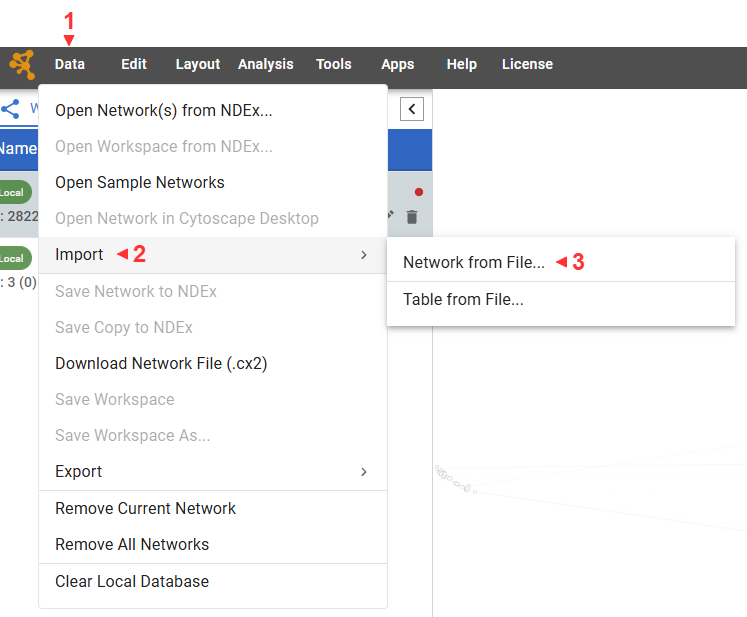
\includegraphics[keepaspectratio]{img/lab4/cytoscape_load.png}}

Let's use the edge weights to fade the less important edges.

\pandocbounded{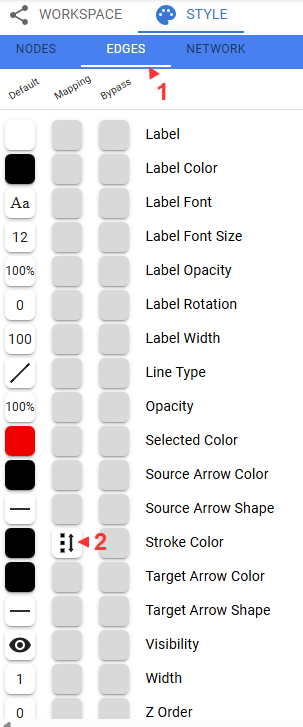
\includegraphics[keepaspectratio]{img/lab4/cytoscape_edge1.png}}

\pandocbounded{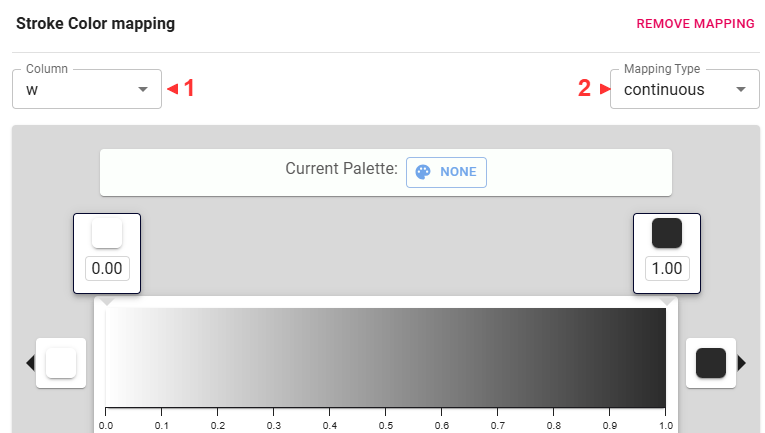
\includegraphics[keepaspectratio]{img/lab4/cytoscape_edge2.png}}

Some useful navigational tips:

\begin{itemize}
\tightlist
\item
  Scroll to zoom.
\item
  Click and drag to pan.
\item
  Nodes can be dragged around
\item
  Multiple nodes can be selected by pressing shift, clicking, and dragging a box.
\item
  Node properties are shown in a table at the bottom
\end{itemize}

Play with mapping other values to different visual aspects of the network.
Save your network with \texttt{Data\ -\textgreater{}\ Download\ Network\ File\ (.cx2)}

This concludes the lab!

  \bibliography{book.bib,packages.bib}

\end{document}
